\documentclass[a4paper,10pt,onecolumn,oneside,openany]{jsbook}
% 参考URL http://d.hatena.ne.jp/yosshi71jp/20101210/1292005429 感謝です
% パッケージの設定,これは不要なものもあるかもしれない
\usepackage{amsmath,amssymb}
\usepackage{bm}
\usepackage{epsbox}
\usepackage[dvipdfmx]{graphicx}
\usepackage{verbatim}
\usepackage{wrapfig}
\usepackage{ascmac}
\usepackage{makeidx}
\usepackage[dvipdfmx]{graphicx}

\usepackage{listings, jlisting}
\usepackage{color}
 
\lstset{
    language=Python,%プログラミング言語によって変える。
    numbers = left,
    numberstyle = {\tiny \emph},
    numbersep = 10pt,
    breaklines = true,
    breakindent = 40pt,
    frame = tlRB,
    frameround = ffft,
    framesep = 3pt,
    rulesep = 1pt,
    rulecolor = {\color{black}},
    rulesepcolor = {\color{black}},
    flexiblecolumns = true,
    keepspaces = false,
    basicstyle = \scriptsize,
    identifierstyle = \itshape\scriptsize,
    commentstyle = \fontfamily{ptm}\selectfont\scriptsize,
    stringstyle = \scshape\scriptsize,
    tabsize = 4, 
 }

\makeindex
%%% 余白・文字数調整(左37mm, 右18mm, 上下共30mm, 文字数約40字/行, 行数約32行)
% 実際の寸法は学科の規定に従ってくださいね
\setlength{\textwidth}{155truemm}      % テキスト幅: 210-(37+18)=155mm
\setlength{\fullwidth}{\textwidth}     % ページ全体の幅
\setlength{\oddsidemargin}{37truemm}   % 左余白
\addtolength{\oddsidemargin}{-1truein} % 左位置デフォルトから-1inch
\setlength{\topmargin}{30truemm}       % 上余白
\setlength{\textheight}{237truemm}     % テキスト高さ: 297-(30+30)=237mm
\addtolength{\topmargin}{-1truein}     % 上位置デフォルトから-1inch
% 本文の行数と桁数を指定出来るように
\def\linesparpage#1{\baselineskip=\textheight
   \divide\baselineskip by #1}
\def\kcharparline#1{%
   \ifx\xkanjiskip\undefined%
   % NTT jTeX用
   \jintercharskip 0mm plus 0.2mm minus 0.2mm
   \else
   % ASCII pTex用
   \xkanjiskip 0mm plus 0.2mm minus 0.2mm
   \fi
   \settowidth{\textwidth}{あ}%
   \multiply\textwidth by #1}
%
%
\begin{document}
\linesparpage{32} % 一ページを32行に(効果ない・・・)
\kcharparline{40} % 一行を40字に
%%% タイトル設定
\begin{titlepage}
\begin{flushleft}
{\large
2016年度 卒業論文 \\ 
}
\end{flushleft}
\begin{flushright}
{\large
指導教員:来住伸子 教授 \\ % 主査
%副査:□□□□ 教授              % 副査
}
\end{flushright}

\begin{center}
\vspace{150truept}
{\huge Scratchプログラムの可視化による類似度推定}\\ % タイトル
%{\huge 可視化によるScratchプログラムの理解支援}\\ % タイトル

%\vspace{10truept}
%{\Large subtitle}\\ % サブタイトル(なければコメントアウト)

\vspace{80truept}
{\huge 津田塾大学 学芸学部 情報科学科}\\
\vspace{30truept}
{\huge G13908 岩科智彩}\\ % 学籍番号 著者
\vspace{10truept}
{\huge G13924 森下汐美}\\ % 学籍番号
\vspace{50truept}
{\huge 2017年1月13日}\\ % 提出日
\end{center}
\end{titlepage}

\frontmatter
\begin{abstract} %論文要旨
\subsubsection{概要}
近年プログラミング教育が推進され、学校での義務教育化が進んでいる。プログラミング教育の方法の1つとして挙げられているのが、米国マサチューセッツ工科大学のメディアラボが開発したScratchである。これは、無償で提供されているグラフィックプログラミング環境を指し、プログラミングを行う際の命令をブロックを組み合わせることで作り上げる。初心者にとっては使いやすい構造となっているため米国では利用者が増えているものの、日本のユーザーは全体の1\%にも満たない。そこで実際に本ツールで公表されているデータを利用して、より教育現場で用いられるようなツールを目指すためにデータ解析を行う。
本ツールではすでに
\begin{enumerate}
  \item 全ユーザにおける各ブロックの種類の使用率
  \item あるプロジェクトの他ユーザーへの引用関係を示したツリー構造
\end{enumerate}
が公表されている。しかしこのデータは全体像の把握が可能であるものの、1つのプログラムにおけるブロックの使い方や、引用していた場合引用元からの変更の程度などは読み取ることができない。
従って本研究では1つのプログラムで使用されているブロックを解析し結果を出力すると同時に引用元との比較を行い、類似性を導き出す。
\end{abstract}

%%% 目次
\tableofcontents
%
%
\mainmatter
%
%%% 本文ここから

\part{序論} %3部構成を取る必要がない場合もあります
\chapter{はじめに}
\section{本研究の背景}

2006年に開発されたScratchというビジュアルプログラミング環境がある。本研究ではScratchのデータを用いて教育の場で役立てる方法を導き出す。Scratchとは米国マサチューセッツ工科大学のメディアラボが開発したフリーツールであり、キーボードでコードを打つのではなくパズルのようにブロックを組み合わせてプログラムの完成させる。
近年、世界ではIT化が進み、物とインターネットを繋ぐIoTが次々と増えていく中エンジニア不足が叫ばれている。しかし世界的に見るとプログラミング分野では日本は遅れている。総務省平成26年度「教育・学習分野の情報化に係る国内外の動向と先進事例」では世界各国でプログラミング教育が活発化していることが分かる(資料{itedu})。日本の旧学習指導要領の必修科目では、パドコンでワードやエクセルの使い方の教育しか行っていないが、イスラエルではコンピュータの使い方よりも原理やプログラミングを教える教育が行われている。
そのため文部科学省が2016年5月19日に発表をした成長戦略素案では第4次産業革命を支える人材を強化するため情報活用能力を伸ばそうと2020年度から小学校、2021年度に中学校、2022年度には高校でプログラミング教育での必修化の予定されている。それに先駆けて国内の学校では実際にプログラミングを行う授業も増えているという(\cite{edu_prog})。品川区立京陽小学校では2014年度よりScratchが導入され各教科の中で活用されている。例えば理科の授業で実験結果をシミュレーションするプログラムの作成にScratchが用いられているようだ。
\begin{figure}[h]
  \centering
    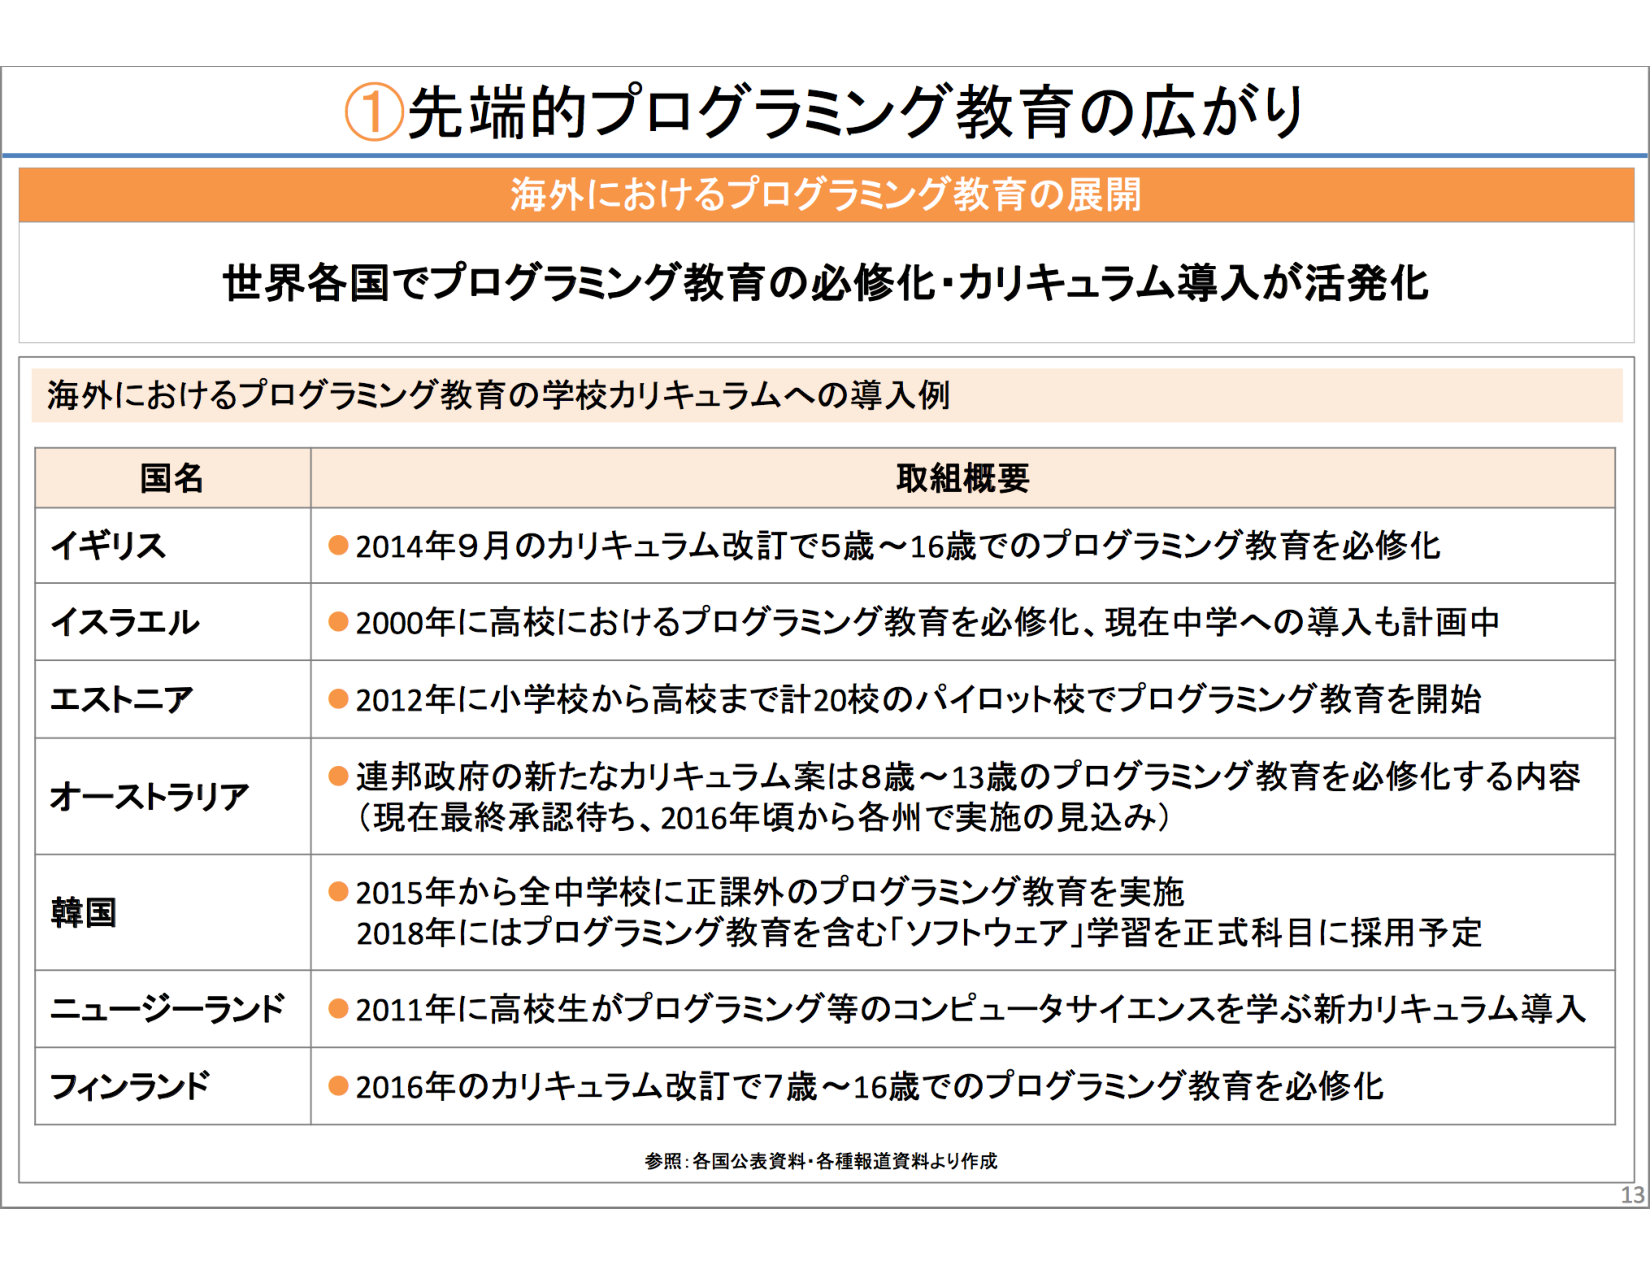
\includegraphics[scale=0.4]{graphic/foreign_data.pdf}
  \caption{平成26年度総務省 教育・学習分野の情報化に係る国内外の動向と先進事例}
  \label{itedu}
 \end{figure}
 
\begin{figure}[h]
  \centering
    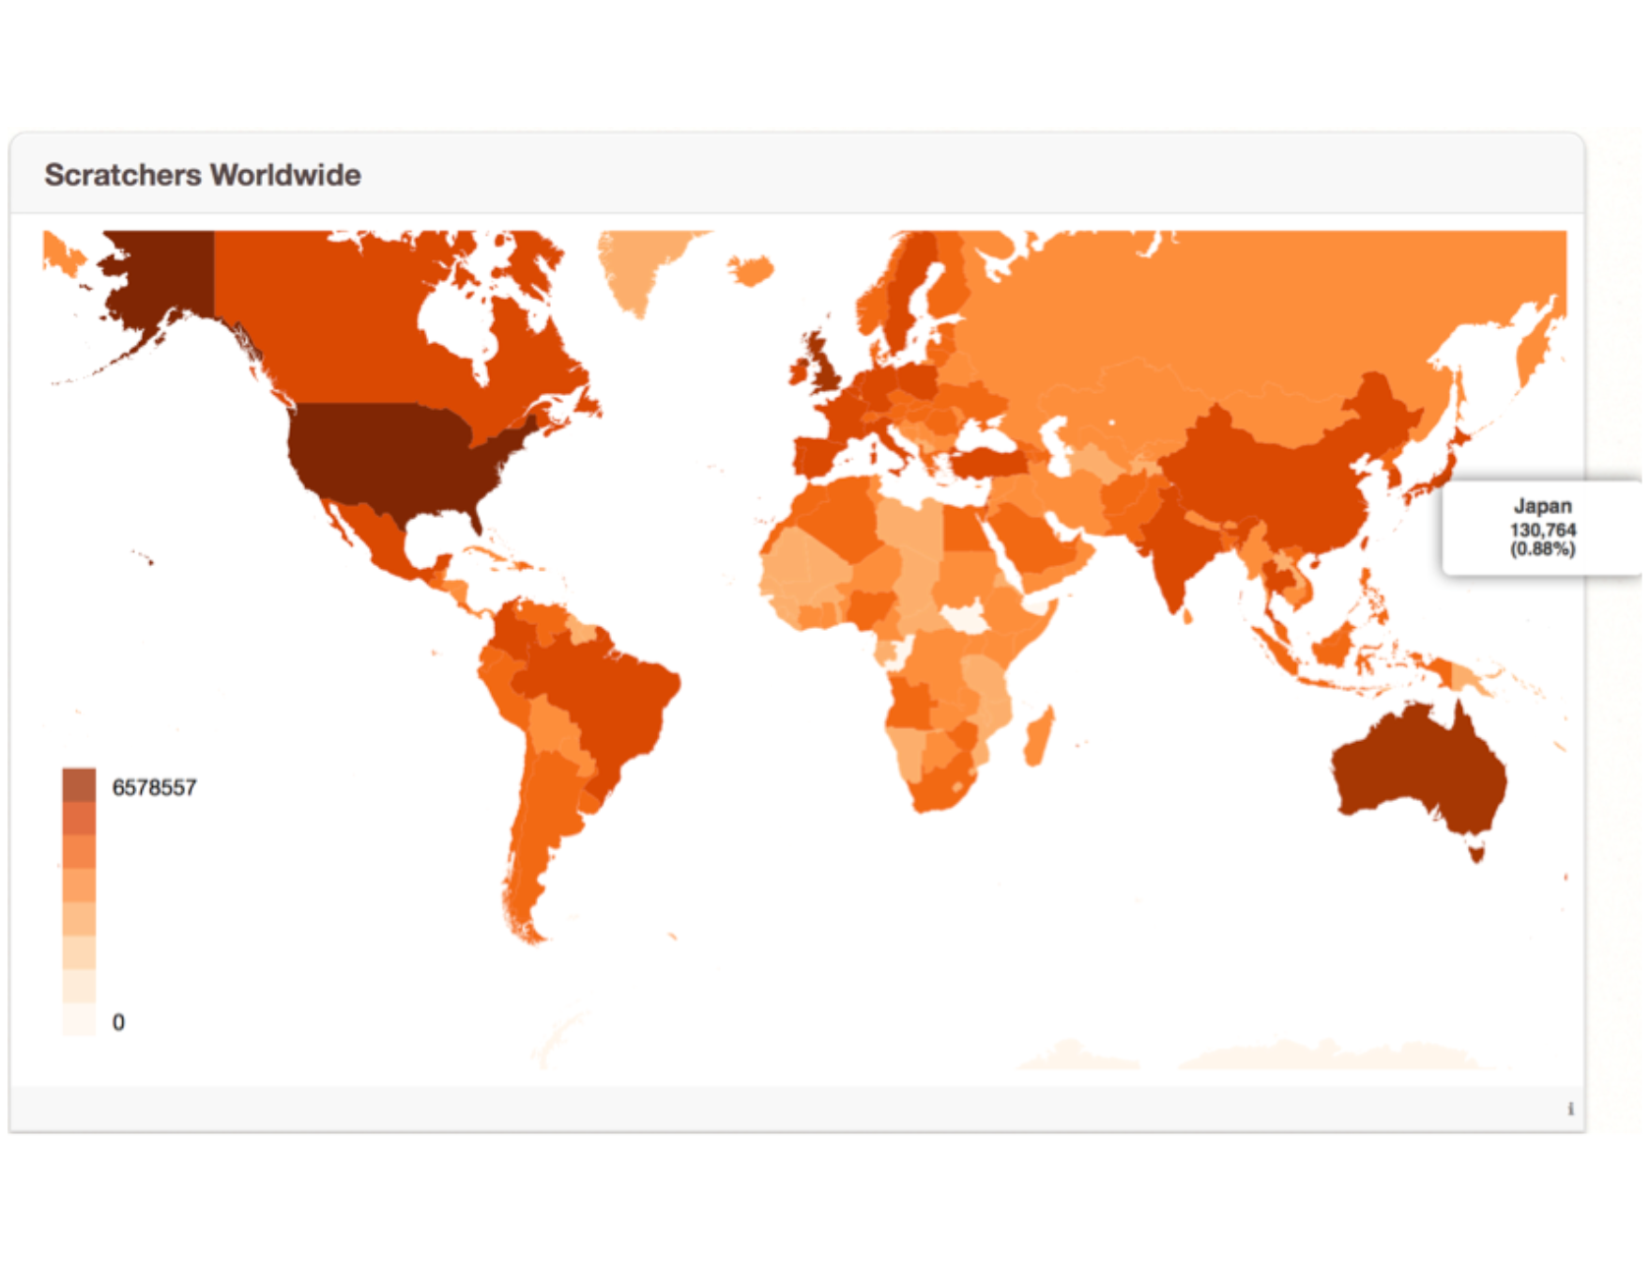
\includegraphics[scale=0.4]{graphic/world_japan.pdf}
  \caption{全世界のScratchユーザー 日本 130,764人 0.88\%}
  \label{num}
\end{figure}

Scratchでは全世界のユーザーのうち日本でのユーザーは現状で1\%(資料\ref{num})である。Scratch公式では利用者の数、年齢、使っているブロック等の統計データの公表があるが、Scratch自体を題材にしている先行研究は日本では数が多くない。そこで義務教育化に伴い日本でも教育現場でScratchを導入しやすくするため公開されているプログラムやデータを利用して解析を行う。

\newpage
\section{本研究の目的}

本研究ではScratchで公開されているプログラム、統計データを利用して分析、実験を実施する。その中でも公開データであるリミックスツリーの精度を検証し、実際に使い易いデータの可視化であるかどうかを評価する。その結果を用いてプログラミング教育における課題点を解決を目指す。

\chapter{先行研究}
\section{先行研究1}
\subsection{概要}
奈良女子大学附属小学校の4年生でScratchを使った授業を行い、この授業を通してScratchの導入について評価している。
\\
 研究方法として、「Scratchのコマンド探し」、「図形を描く」、「作品づくり1」、「作品づくり2」の4つのフェーズに分けて授業を進める。「作品づくり1」は個人作業、「作品づくり2」はグループ作業となっている。提出された作品は、ブロック数やスプライト数、使用されているブロックの機能別分布、さらに一つ一つのブロックの使用割合などを集計し、最後にブロックの理解度と利用率についてまとめている。
\\
 これらの評価を踏まえ、Scratchを授業に取り入れることで、条件分岐やキー入力の判別処理のような複雑なプログラミングを使用して作品を作ることができた児童が8割を超え、プログラミング導入の目的を達成することができたとまとめている。(\cite{preEssay1})

\subsection{評価}
この研究は、実際に児童を対象にScratchでの授業を行い、このツールがプログラミング導入に適切かどうか評価している。評価の中で、ブロック数やスプライト数などいくつかのデータを収集し、児童がどれだけブロックを使用できているかを調査しているが、児童が作った作品同士の類似度を分かりやすく可視化まではできておらず、本研究を行うことで改善できるのではないかと考えている。可視化を提案することで、児童ごとの進度をより分かりやすく示すことができ、授業内で役立てられるのではないかと期待している。
\section{先行研究2}
\subsection{概要}
Scratchプログラム間の類似度を数字で表す方法を知るため、2011年度の神戸市立工業高等専門学校電子工学科よりPascal言語のプログラムを利用し類似性を定量化する研究を参考にする。先行研究では学校の課題で提出される学生のプログラムは似た動きをするためほとんど同じのことが多いため類似性を機械的に抽出ができるのではないかと仮定している。類似度の計算を新しく提案したカーネル法を基にして算出し、実際の結果をクラスタに分けどのような特徴を持つ手法であるかを調査している。\cite{preEssay2}
\subsection{評価}
本研究と先行研究では題材であるプログラムの形が違うが、Scratchプログラムでは要素同士がリスト化されているJSON形式であるため類似度の計算手法を別のものに変更して行えると考える。またクラスタが可視化されたグラフが先行研究である様に本研究でも可視化をすることでScratch公式サイトにて公表されているグラフィックを上回る結果を目標とする。


%\section{本論文の構成}


\part{本論}

%ちさちゃん
\chapter{Scratchについて}
\section{Scratchとは}
Scratchとは、プログラミングを学ぶ子どもや初心者が、構文の書き方や使い方を覚えることなく結果を得ることができる、プログラミング言語学習環境である。2006年にMITメディアラボのミッチェル・レズニックが主導するライフロング・キンダーガーデン・グループによって開発された。プログラミングを可能な限り簡単に学べるよう、視覚表現でキャラクターを動かすことができ、ビジュアルプログラミングとも言われている。
\section{Scratchの使い方}
Scratchの公式サイト(\cite{scratch})にアクセスしてオンライン上で使用することができる。(2013年5月にリリースされたバージョン2.0からウェブアプリケーションも出ている)またScratchのダウンロードサイト\cite{scratch_official}
よりパソコンにダウンロードすることで、オフラインでも楽しめる。ここではオンライン上での使い方を説明する。初めて使用するときはページ上部の「Scratchに参加しよう」というボタンをクリックし、ユーザ登録を行う。ユーザ登録を行うことでできあがった作品はオンラインコミュニティで他のユーザと共有することができる。
 同じくページ上部の「作る」というボタンをクリックすると、開発環境(図\ref{editor})が表示される。ページ左側が実行結果を表示し、右側がプログラムを書く部分である。左側の画面にいるネコはデフォルトで設定されているキャラクターで、スプライトと呼ばれている。このスプライト一つ一つにブロックを積んでいくことで実際に実行することができる。
\begin{figure}[!h]
  \centering
    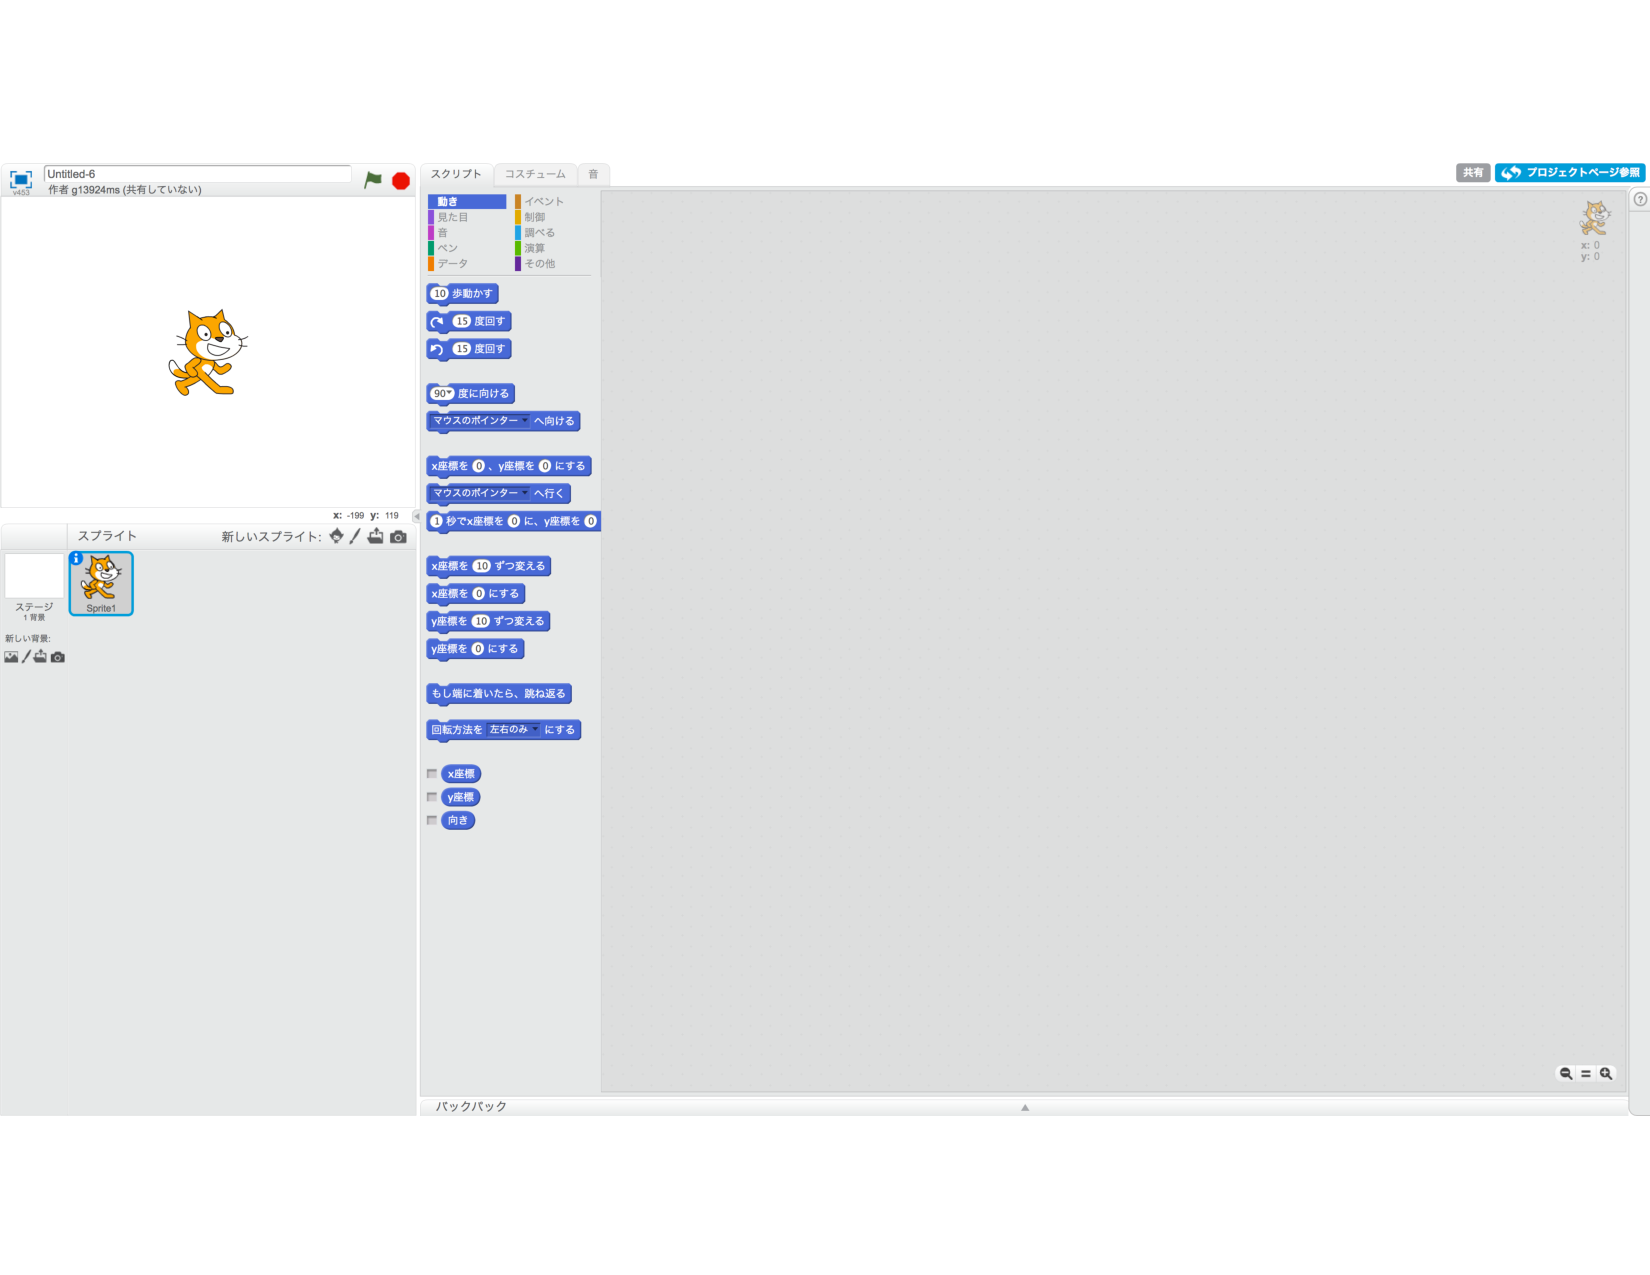
\includegraphics[scale=0.5]{scratch_editor_main.pdf}
  \caption{Scratchプロジェクト作成画面}
  \label{editor}
 \end{figure}
 プログラムの命令にあたるのが、ブロックである。ブロックは、動き・見た目・音・ペン・データ・イベント・制御・調べる・演算・その他の種類に分かれており、それぞれの機能に応じてブロックを組み合わせることができる。(図\ref{pseditor})例えば、「画面上の緑の旗のマークが押されたときにスプライトが10歩動く」というプログラムを構成したいときは、イベントと動きのブロックを組み合わせることで、実行できる。
 \begin{figure}[!h]
  \centering
   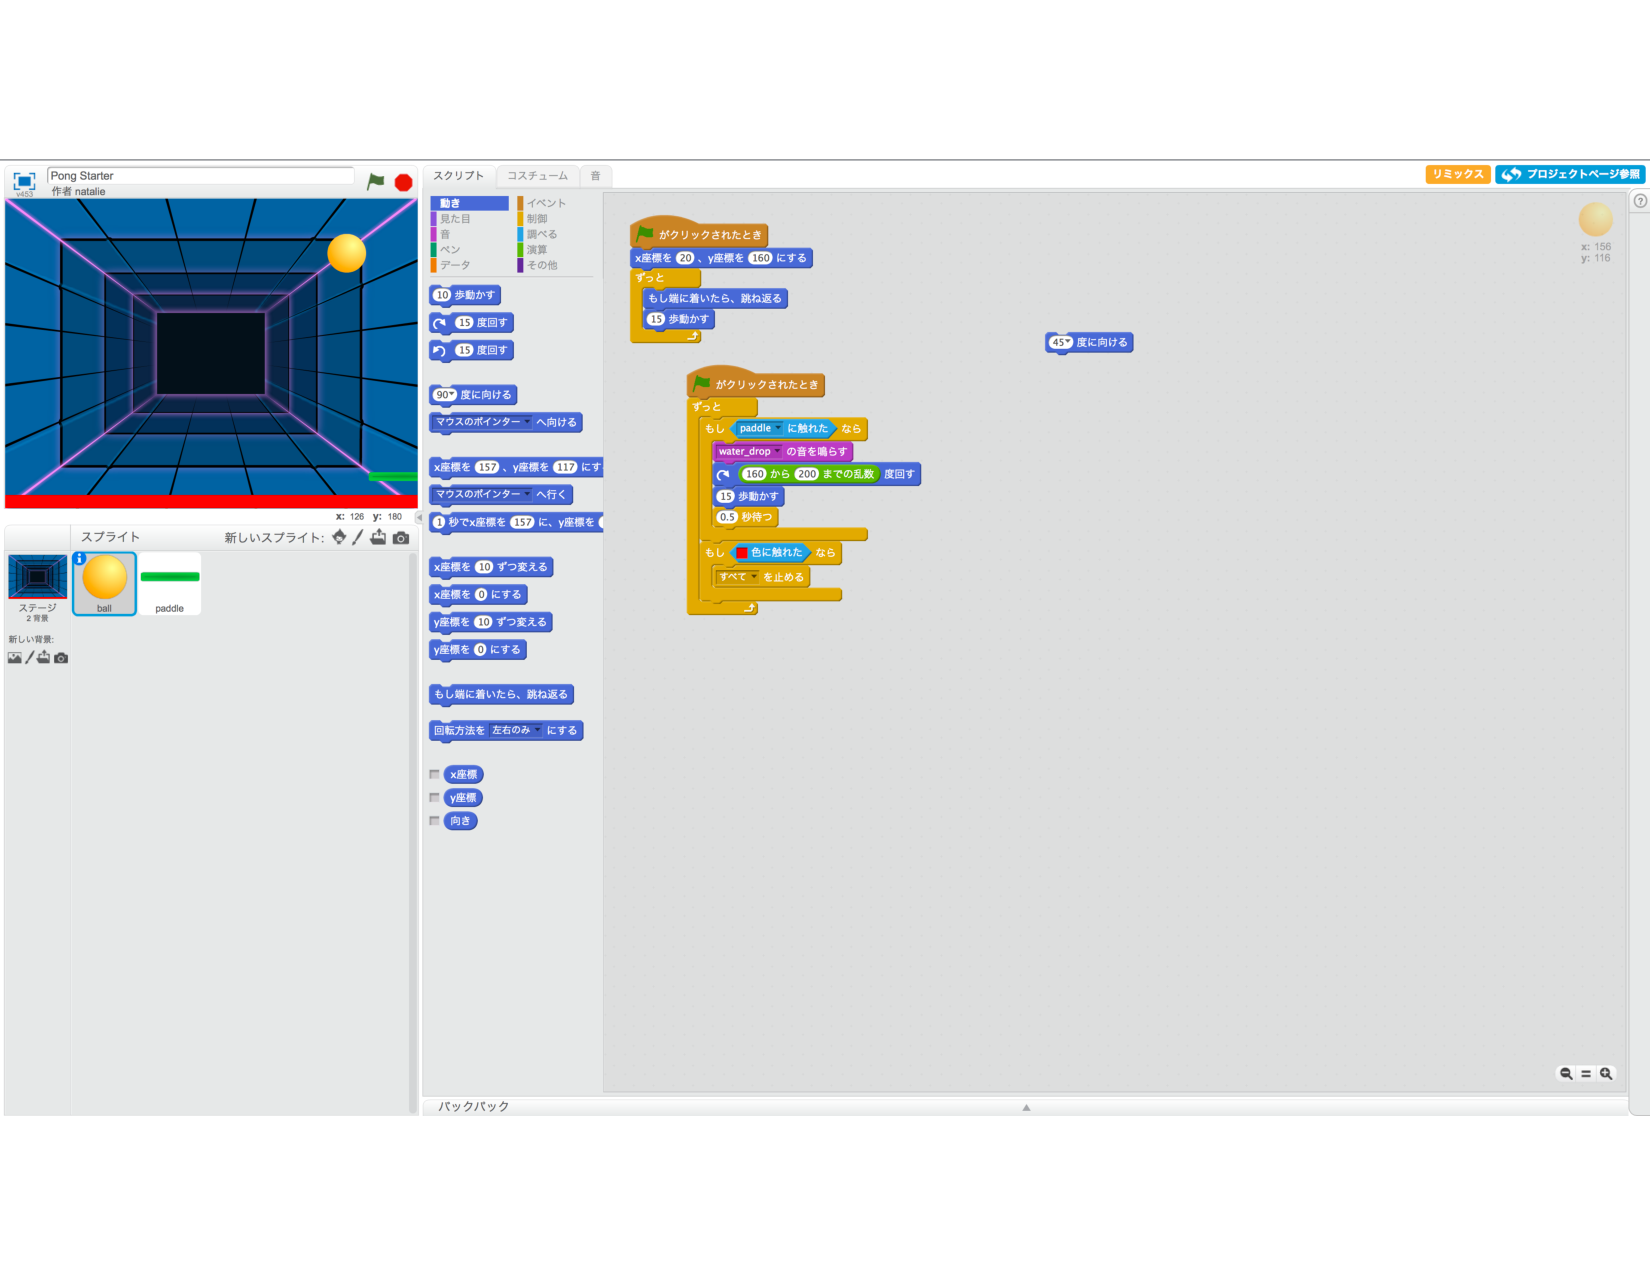
\includegraphics[scale=0.5]{pong_starter_editor.pdf}
  \caption{Pong Starterプロジェクト編集画面}
  \label{pseditor}
 \end{figure}
 他のユーザの作品を見たいときは、「見る」というボタンをクリックする。アニメーションやゲームなど、さまざまなジャンルの作品を見ることができる。他のユーザの作品を見てみると、ページ下部の一番左に木のマークがあり、その横に数字が書かれている。ここをクリックして開いてみると、ひとつの木が現れる。これはリミックスツリーというもので、このプログラムはどれだけのユーザが参考にしたのか、引用したのか、可視化されたものである。Scratchは簡単に他のユーザの作品をコピーすることができるが、それは誰かの作品を引用し作っていくことを大事にしているからである。このリミックスツリーはのちの研究の中で紹介する。
\section{Scratchの特徴}
Scratchの最大の特徴は視覚的な分かりやすさである。プログラムの構文や文法などを理解できなくても、ブロックの機能と適切なブロックを選び組み合わせることで簡単に実行させることができる。ブロックも機能ごとに色分けされ、役割を認識しながらプログラムを組み立てることができる。また繰り返しの構文や条件文などプログラム構文の基礎となるアルゴリズムの考え方もScratchを使用しているうちに少しずつ慣らしていくことができる。(\cite{scratch_article}) 作成できる作品の種類として、ゲームや動画制作、対話式のプログラムを得意とする。要因の一つとして、ビジュアルプログラミングであることが挙げられる。またScratchは一つのコミュニティサイトとしても見ることができる。公開した作品のユーザの反響の確認が可能であり、それを参考に改良したり、よりよいプログラムを見つけるとそれをそのままコピーするしたり、それを元にオリジナル作品を生み出すことができる。
 一方、ブロックを使用することでプログラム構造の概念は簡単に学ぶことができるが、実際のJavaやCなどのプログラミング言語の習得とは同様ではない。プログラム入門の一つの壁であるキーボード操作が分からない場合でも手軽に体験できるものであり、実際に言語を使って行うプログラミングとは異なる。またScratchを構成する%ちょっとよくわからないこの文
元々要素が古く、加えてScratchの延長となるプログラミング言語がないことも理由に挙げられる。独立した言語であるために将来的な応用をつけるのは容易ではない。
\section{Scratchの利用度}
Scratchは元々8歳から16歳の子ども向けに作られたツールであるが、現在すべての年代のプログラミング初心者に使われている。Scratch公式サイト\cite{scratch_about}によると150以上の国で使用されており、40カ国語以上に翻訳されている。ツール上で簡単に翻訳できるようになっている。また、学校での利用も多い。小学生から大学生まで幅広い年代の学生が情報の授業などで使用している。
\section{本研究におけるScratchの利用意義}
まず、学校教育でよく使われていることが挙げられる。日本ではまだ少ないが、世界的に見るとこのツールを使って授業をしているところが多く、これからの日本の情報教育の義務化にあたって、Scratchの機能がこれからの日本の情報教育の方針に一番近いと考えられる。また、Scratchの特徴の一つに、他のユーザの作品を参考にするためにコピーが簡単にできるとあった。これは、他の作品で使われている新たなブロックの組み合わせ方や定義などを学び、自分の作品で使えるようにするためである。この仕組みが情報教育で役に立つと考える。そして、このツールは世界中のユーザが存在し、その分公開されているプログラムの数が多く、十分なデータを得ることができる、そしてそのデータがネット上で簡単に入手できるため本ツールを使用する。

%しおみ
\chapter{Scratch公式可視化データの現状}
\section{ブロックの利用度}

Scratch公式では無作為に選ばれたプログラムで使用されているブロックの種類を集計し、項目ごとに色を分けて利用度を可視化してある。高い割合の項目ほど面積が大きい。(図\ref{blockan})
 項目をクリックすると利用度の高いブロックが同じように面積が大きく表示される。(図\ref{blockdit}) このデータではScratch全体で使われているブロックの利用度の把握が可能である。しかしユーザー個人個人が作成したプログラムのブロックの利用度が分かるということではない。
 
\begin{figure}[ht]
  \centering
    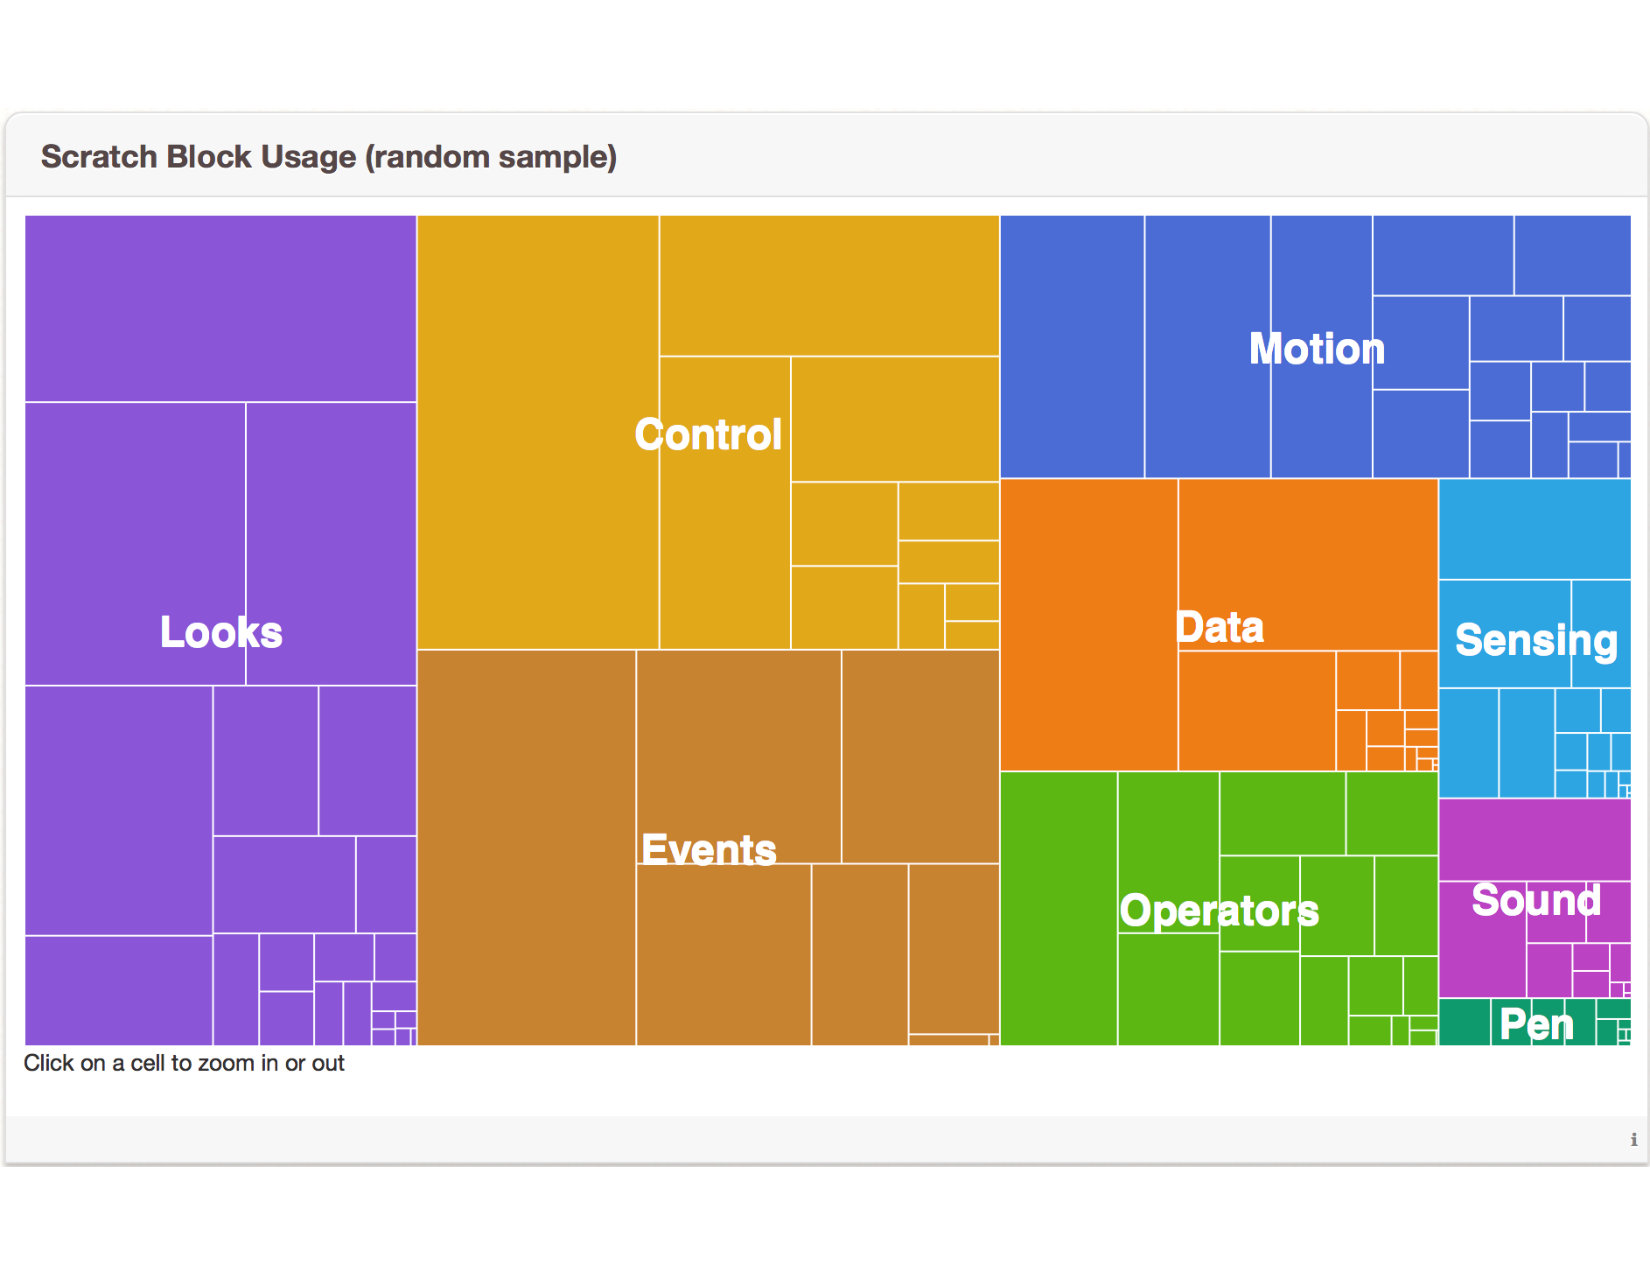
\includegraphics[scale=0.5]{graphic/scratch_block0.pdf}
  \caption{全ユーザーブロック利用度}
  \label{blockan}
 \end{figure}
 
 \begin{figure}[ht]
  \centering
    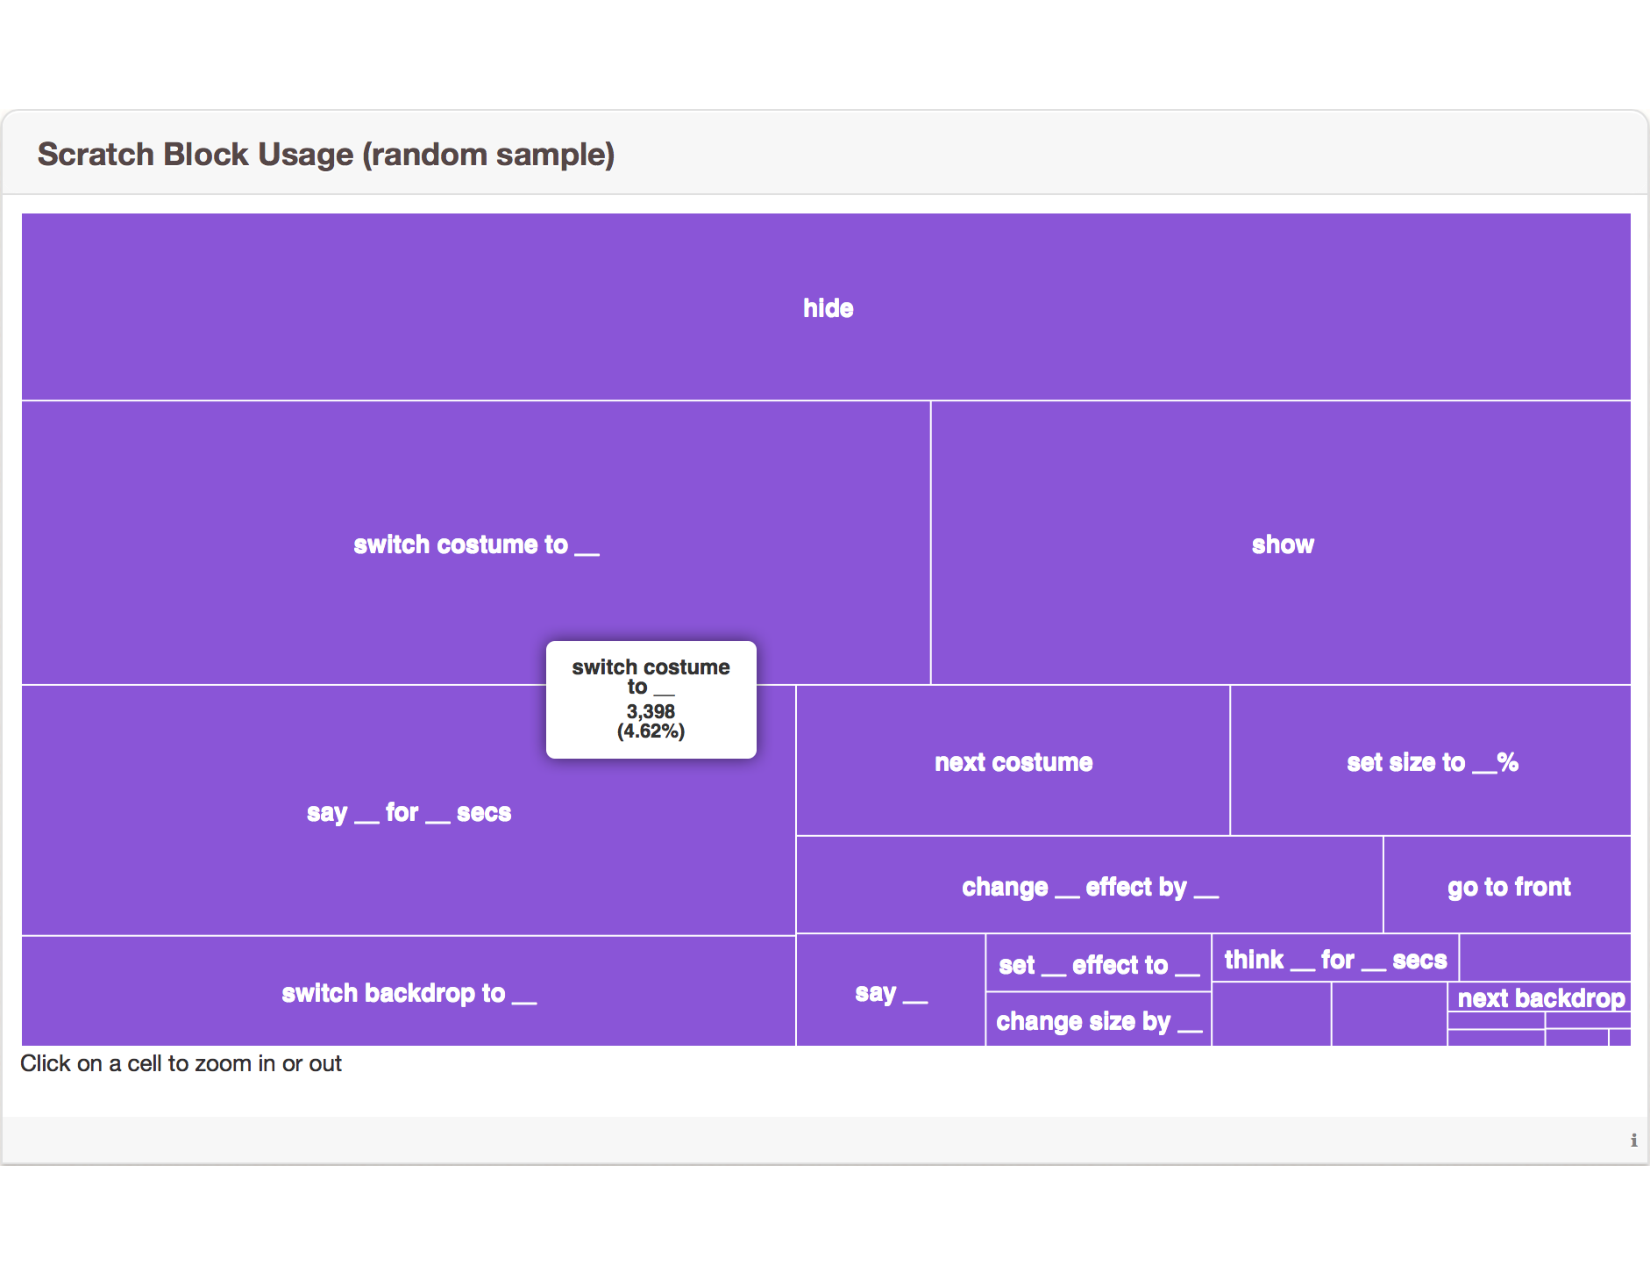
\includegraphics[scale=0.5]{graphic/scratch_block.pdf}
  \caption{全ユーザーブロック利用度 Locks(制御ブロック)をクリックした時}
  \label{blockdit}
 \end{figure}
 
 
\newpage
\section{リミックスツリー}
木構造になっているリミックスツリーは根元のプログラムを元として引用関係を表している。(図\ref{psrt})さらに引用されたプログラムを引用した場合も反映される。(図\ref{rtdit})この図はどのくらい変更が加えられているかがわからない点から元のプログラムと先端のプログラムの差を把握することは難関である。

\begin{figure}[ht]
  \centering
    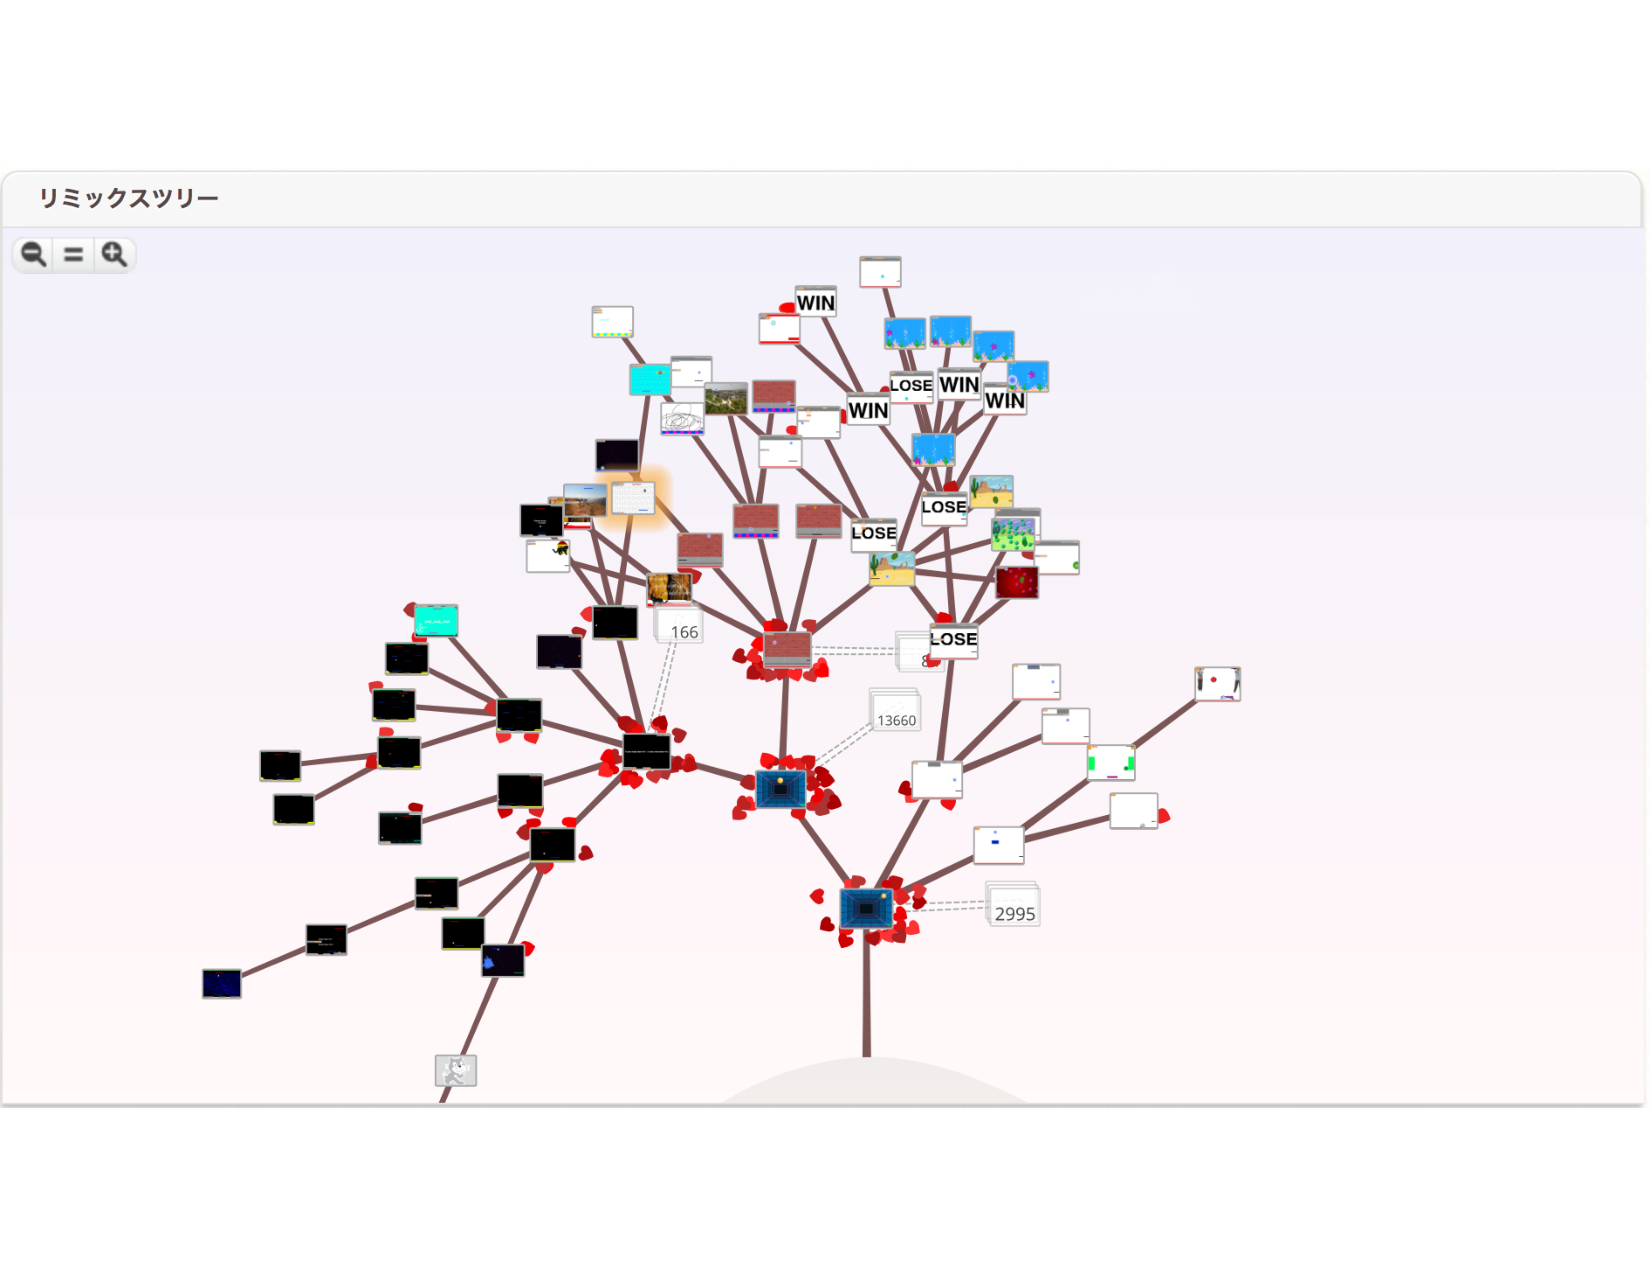
\includegraphics[scale=0.5]{graphic/remixtree_all.pdf}
  \caption{Pong Starter のリミックスツリー}
  \label{psrt}
 \end{figure}

\begin{figure}[hb]
  \centering
    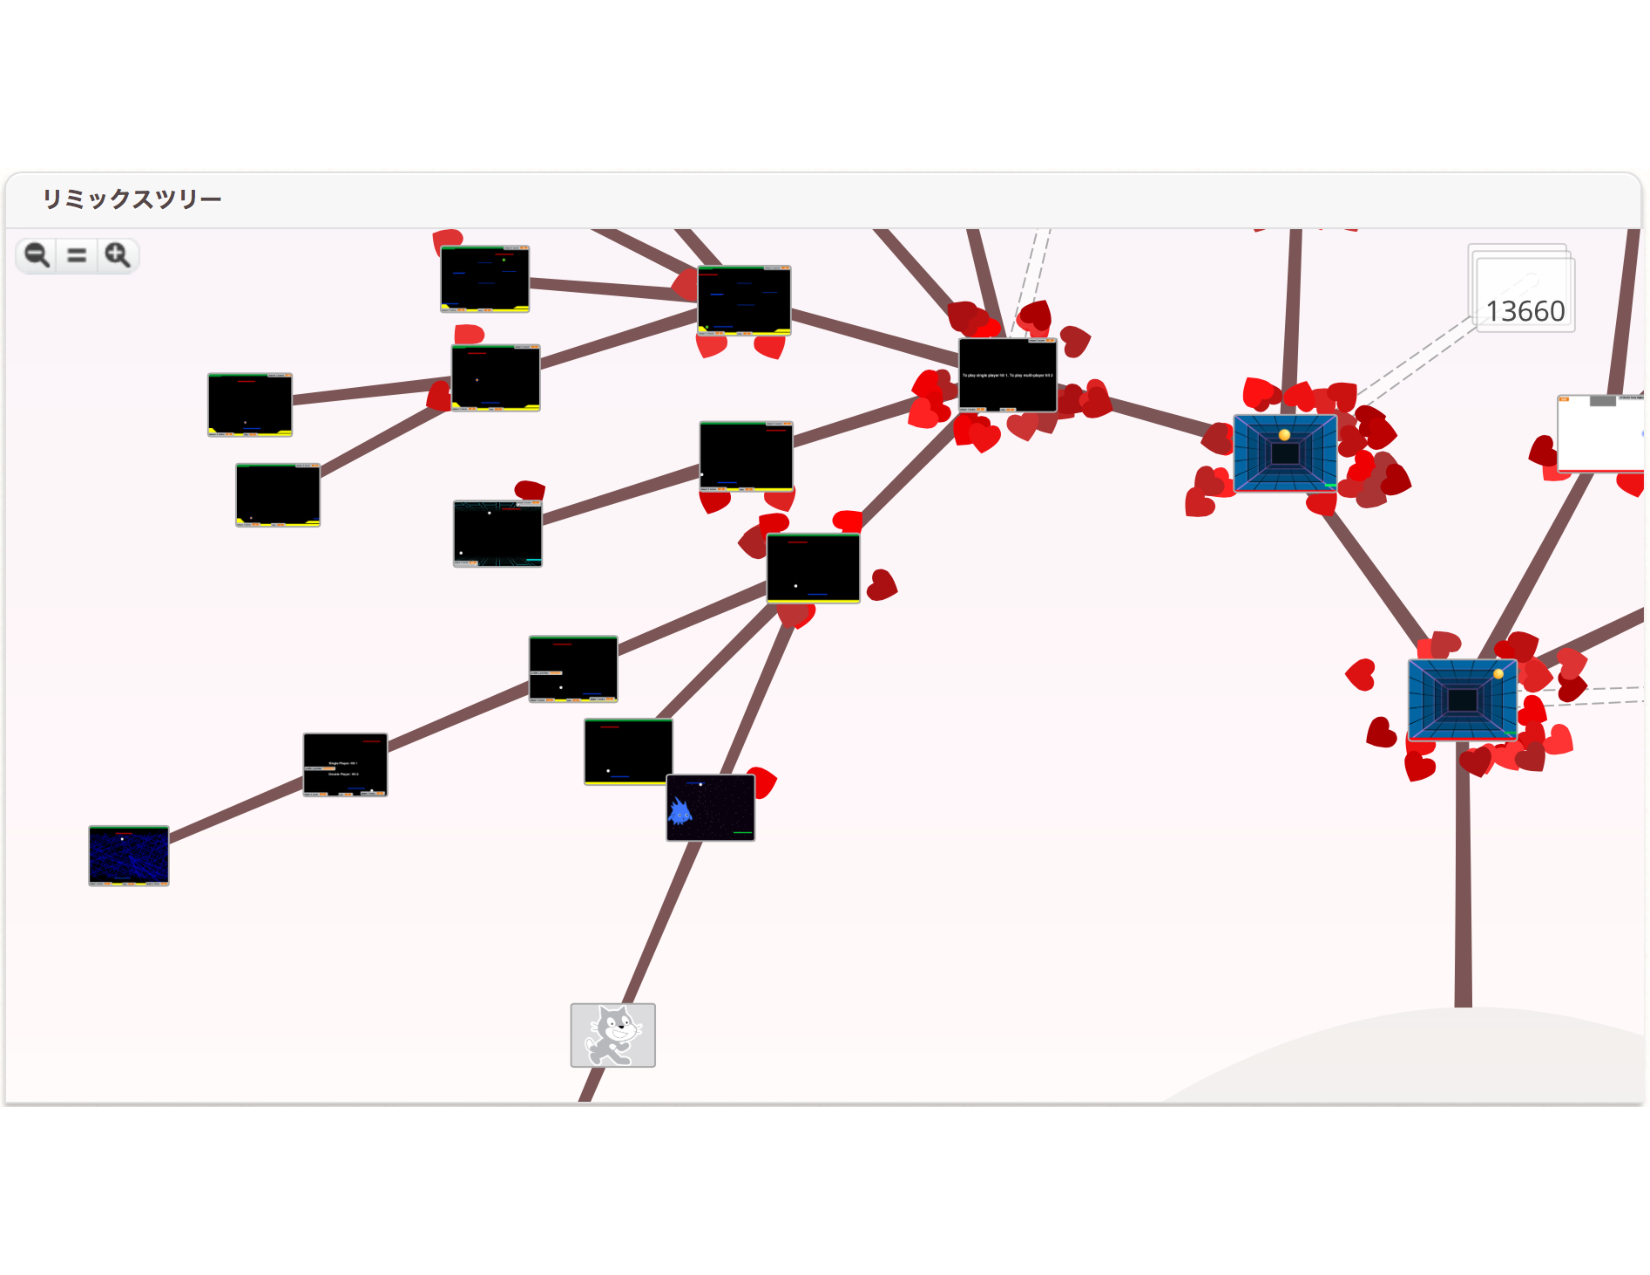
\includegraphics[scale=0.5]{graphic/remixtree_detail.pdf}
  \caption{Pong Starter のリミックスツリー 左下詳細}
  \label{rtdit}
 \end{figure}

 

\chapter{研究内容}
\section{問題提起}
前章で挙げたリミックスツリーの可視化では元のプロジェクトから引用した新たなプロジェクトは引用したという結果が表されており、全て同じ距離になっている。(\ref{remixtreedis})
つまり何も変更が加えられてないプロジェクトとかなり改造されたプロジェクトの違いは可視化されない。学ぶ側はレベルの把握、教える側には評価をしやすいくするために変化の度合いの可視化を可能にする。
 \section{実験方法と仮説}
本研究では2万弱の引用がされている"Pong Starter"プロジェクトのリミックスツリー(\cite{pongret})を利用する。まず元のプログラムから引用されたものを1段目とする。以後1段目のプロジェクトから引用されたものを2段目、2段目から引用されたものを3段目とする。それらを順に元のプロジェクトと比較をしていき、使われたブロックの数、スプライト(オブジェクト)の数、類似度を表すcos類似度の数値化、グラフ化をする。リミックスツリーで表されているのは引用関係であるため、実際に1段目にあるものより3段目のものの方が元のプロジェクトと類似しているまた逆の結果が表れることが予測される。
\newpage
 \section{技術の解説}
\subsection{使用するプログラミング言語}
本研究ではScratch公式サイトよりプロジェクトをJSON形式でインポートし、Pythonを利用してデータを抽出、分析を行う。
\subsubsection{Pythonとは}
PythonはGuido van Rossum氏の作成した軽量プログラミング言語である。記述や取り回しが容易であり、コンパイルも不必要という特徴がある。(\cite{python})
 \begin{lstlisting}[caption=C言語,label=clan]
 void main()
 {
 	printf("Hello World!");
	return 0;
}
 \end{lstlisting}
 
 
 \begin{lstlisting}[caption=Python,label=python]
 print("Hello World!")
 \end{lstlisting}
 
文法はC言語やJavaとは異なり、中括弧を使用せずインデントでのブロック構造になっている。これは誰がコードを書いても同じソースコードになることがわかり、可読性に優れている。このような習得のしやすさから教育の場では広く使用されてきていることも分かった。
\subsubsection{JSONとは}
JSONはJavaScript Object Notationの略であり、テキストベースのデータフォーマットである。表記の基はJavaScriptであるだけでそれ以外では、記述が容易であり可読性に優れているため他のプログラミング言語でも利用可能である。基本は数値とその名前(キー)をペアにしてコロンで対になっている。項目はコンマで区切られ、全体は中括弧で区切られる。(\cite{json})

PythonではjsonモジュールをインポートすることでJSON形式ファイルを読み込むことが可能であり、Pythonでは辞書型に保存される。(\cite{json_py})次節ではPython環境でのJSONデータの操作するプログラムの説明をする。

 \begin{lstlisting}[caption=JSON,label=json]
 {
 "book1":{
"title": "Python Beginner",
 "year": 2013 ,
"page": 349
},
"book2":{
 "title": "JSON Beginner",
 "year": 2003 ,
"page": 640
 }
}
 \end{lstlisting}
 
\subsection{プログラムの解説}
本研究では2つのプログラムと1つの辞書データを使用する。ソースコード\ref{saprog}はブロック、スプライトの数、cos類似度を計算結果を出力する。ソースコード\ref{scprog}はcos類似度を実施に計算するプログラムとなっている。共通するブロックの名前の個数である値の積を分子、値の自乗をブロックの種類分足してルートをかけたものをA,Bそれぞれ計算しかけたものを分母として、割り算を行い、cos類似度を求めている。
\subsubsection{cos類似度とは}
cos類似度とはベクトル空間モデルにおいて、文書同士を比較する際に用いられる類似度計算方法である。
\begin{quote}
コサイン類似度は、そのままベクトル同士の成す角度の近さを表現するため、三角関数の普通のコサインの通り、1に近ければ類似しており、0に近ければ似ていないことになる。(\cite{cos})
\end{quote}
【数式】
\begin{equation}
\cos(A,B) = \frac{\vec{A} \ast\vec{B}} {|\vec{A}||\vec{B}|}  = \frac{\vec{A}}{|\vec{B}|}\ast\frac{\vec{A}}{|\vec{B}|} = \frac{\sqrt {\sum_{i=1}^{|V|}}}{\sqrt{\sum_{i=1}^{|V|}A_i^2\ast\sum_{i=1}^{|V|}B_i^2}}
\end{equation}
\\
【例】(\cite{tf_idf_cos})
\\文章A:「赤と緑、緑と青」
\\文章B:「赤と黄、紫と赤」
\\2つの文章のベクターは赤、緑、青、黄、紫のうちそれぞれ何個使われているかを表す。
\\ベクターA:(赤、緑、黄、青、紫) = (1, 2, 0, 1, 0)
\\ベクターB:(赤、緑、黄、青、紫) = (2, 0, 1, 0 ,1)
\\2つのベクターを数式に当てはめる。
\begin{equation}
A \ast B = 1 \ast 2 + 2 \ast 0 + 0 \ast 1 + 1 \ast 0 + 0 \ast 1 = 2
\end{equation}
\begin{equation}
|A| = \sqrt{( 1 \ast 1 + 2 \ast 2 + 0 \ast 0 + 1 \ast 1 + 0 \ast 0 )} = \sqrt{6}
\end{equation}
\begin{equation}
|B| = \sqrt{( 2 \ast 2 + 0 \ast 0 + 1 \ast 1 + 0 \ast 0 + 1 \ast 1 )} = \sqrt{6}
\end{equation}
\begin{equation}
\cos\theta = A \ast B \div |A| |B| = \frac{3}{\sqrt{6}\sqrt{6}} = \frac{1}{2} = 0.5
\end{equation}
\\本研究では例”色”に当たる部分を、”ブロックの種類”にして計算を行った。Scratchでは数多くのブロックが用意されており、どのブロックを使用するかによって、まったく異なるプログラムを作成することができる。それぞれのプログラムのブロック数を集計した後、ソートしベクターに直し計算式に適用する。
\subsubsection{SimCalculatorの解説}
cos類似度の計算は次のプログラムで行う。(サンプルプログラム:\cite{simcalc})
\\
ソースコード\ref{scprog}では2つのベクトルの内積を計算するsim\_cosを作る。
\\
sim\_cosではソースコード\ref{saprog}のベクターリストxxxとyyyを引数とし内積の計算をする。v1(xxx)のn番目のブロックと同じものがv2(yyy)にも存在をするとき、変数numeratorに2つを掛け合わせたものを加える。次にそれぞれのベクターの値を二乗していったものの合計の平方根を掛け合わせたものが分母となるため変数denominatorと置く。最後にnumeratorをdenominatorで割ったものを返す。

\subsubsection{scratchAnalysisの解説}
プログラム\ref{saprog}では始めに使用するモジュールの読み込みをする。jsonデータを使用するためのモジュール(L10)、主にHTTPでURLを開くための関数およびクラスのurllib2モジュール(L11, \cite{urllib})、csv形式(データをカンマで区切ったもの)のデータを扱うことができるcsvモジュール(L12)を読み込む。またscratch\_block(ソースコード\ref{sbprog})を同様に読み込む。このデータファイルはScratchに登場するブロックを辞書型にしたデータファイルscratch\_block.py(\ref{sbprog})であり、キーがブロックの名前、その値は初期値0を指定したものである。最後にcos類似度の計算を行うSimCalculator(ソースコード\ref{scprog})を読み込む。
\\
次に比較するプログラムURLのリスト化したものを読み込む。L31ではバイナリーモードで開いたファイルオブジェクトを変数dataReaderと置く。ファイルを開く際には組み込み関数open()を使用する。(\cite{open}) open()とは開いたファイルをファイルオブジェクトを返す。その際にmodeを2つ目の引数で指定でき、本プログラムでは読み込み専用、バイナリーモードを指定している。このファイルはL141以降のfor文内で改め呼び出す。
\begin{table}[h]
 \caption{【例】URLリストファイル}
 \label{urllist}
 \begin{center}
\begin{tabular}{lclcl}
https://scratch.mit.edu/projects/100275945/ \\
https://scratch.mit.edu/projects/100492744/ \\
https://scratch.mit.edu/projects/100742859/ \\
https://scratch.mit.edu/projects/100821454/ \\
https://scratch.mit.edu/projects/101706154/ \\
https://scratch.mit.edu/projects/101833379/ \\
https://scratch.mit.edu/projects/10190891/ \\
https://scratch.mit.edu/projects/10191205/ \\
https://scratch.mit.edu/projects/10191673/ \\
https://scratch.mit.edu/projects/102090434/ \\
https://scratch.mit.edu/projects/10214982/ \\
https://scratch.mit.edu/projects/102313969/ \\
https://scratch.mit.edu/projects/102381385/ \\
https://scratch.mit.edu/projects/10245234/ \\
https://scratch.mit.edu/projects/102562822/ \\
https://scratch.mit.edu/projects/102589407/ \\
https://scratch.mit.edu/projects/102718914/ \\
https://scratch.mit.edu/projects/102933941/ \\
\end{tabular}
\end{center}
\end{table}
\\
L39 メソッドgetFirstでは読み込んだプロジェクトで使用されているブロックごとの個数を数え、ソースコード\ref{sbprog}の値の上書きを行う。ブロックの総個数を変数countと置く。L41のif文では組み込み関数isinstance()を使用しリストであるかを確認する。(\cite{isinstance}) 組み込み関数のisinstance()とは2つの引数を指定し、1つ目が2つ目のインスタンスであるかどうかを返す。また読み込んだデータリストLが長さ0より大きいリストであれば最初の値を変数firstと置く。L43のif文では同様にisinstance()を使用しリストのキーがUnicode文字列であれば処理を進める。Unicode文字列はバイト単位である通常の文字列に対して、文字型に構わず1文字を1文字として扱う。(\cite{unicode}) if文内では始めに対象データ内の例外処理を行う。ソースコード\ref{sbprog}に記録されているブロック名に一致するように"turnRight:"、"turnLeft:"、"wait:elapsed:from:"の値より末尾のセミコロンを覗く。その際組み込み型のrstripを利用する。rstripはstr.rstripの引数で指定した文字もしくは文字集合を文字列の末尾から覗く。(\cite{rstrip}) L54ではdict内(\cite{sbprog}内の辞書)にfirstと一致するものがあればdictの値を1つ増やす。同時にcountを1つ増やす。L57ではデータリスト内の値をgetFirstの引数に繰り返し置くことで再帰メソッドにする。
\\
次にurllib2モジュールを使用し、Scratchプロジェクトを呼び出す。変数r1でurlを開き、r1.read()でファイルを読み出したものをjson.loadsを使用しjson型のデータをpythonオブジェクトへの脱直列化する。(\cite{loads})  root1より"children"を親とするリスト(y1)を取り出す。L77では取り出したリストy1の長さ分のfor文を作成する。事前に"scripts"を変数aとし(L70)、もしaが含まれていれば、使用されているブロックをL71で定義したリストs1に加える。s1はL99でgetFirstの引数に指定する。L98でソースコード\ref{sbprog}のキーであるblockをxと置く。次にcos類似度の計算をするためのベクターを作る。L106ではxをソートし、xxと置く。初期化したリスト(xxx)にはfor文でキーの値を取得し、書き込んでいく。
\\
次にスプライト数を数える。L86ではスプライト数を数える変数splite\_count1を初期化する。L77のfor文と同様にリストの長さ分、"objName"を持つリストを探し存在すればsplite\_count1の数を1増やす。
\\
L116のfor文では始めに読み込んだcsvファイルに存在するデータURL分繰り返すことにする。ここでは最初に読み込んだプロジェクトと順番に比較していく新たなプロジェクトの計算を同様の方法で行う。for文の最後(L166)では作成したベクターリストxxxとyyyを使い、SimCalculatorより呼び出したメソッドsim\_cosで計算を行う。L176では結果を書き込むcsvファイルを作成する。L177の変数writecsvにwriter()メソッドを指定し、与えられたリストをcsv形式に変換し、返す。L185のbodyリストにはブロックの総数、スプライトの個数、cos類似度をいれ、csv書き込み用のリストcsvlistに格納。L190とL191でL178で指定したcsvの列のラベル名とL186のcsvlistをL176のファイルに書き込む。
\begin{table}[h]
 \caption{【例】結果が書き込まれたファイル}
 \label{resultex}
 \begin{center}
\begin{tabular}{lclcl}
block & splite & cos \\
57 & 2 & 0.622501651 \\
84 & 2 & 0.685970521 \\
116 & 3 & 0.727309832 \\
38 & 2 & 0.788050924 \\
144 & 3 & 0.558885703 \\
108 & 2 & 0.61049762 \\
28 & 3 & 0.939108193 \\
20 & 2 & 0.986013297 \\
19 & 2 & 1 \\
47 & 3 & 0.877613961 \\
69 & 2 & 0.654319919 \\
62 & 2 & 0.662733496 \\
93 & 2 & 0.845819931 \\
61 & 2 & 0.674736483 \\
44 & 3 & 0.917117834 \\
53 & 2 & 0.592156525 \\
35 & 3 & 0.916030755 \\
148 & 10 & 0.910134671 \\
74 & 3 & 0.39669503 \\
93 & 4 & 0.758264769 \\
19 & 2 & 1 \\
21 & 2 & 0.972597525 \\
\end{tabular}
\end{center}
\end{table}


%cos類似度を計算したいjsonプログラムをそれぞれA,Bとすると、A,Bの読み込みを行うとき、プログラムIDを設定することでネット上からプログラムを自動で呼び出せるようにした。プログラムAの中のブロック情報が書かれているchildrenの部分のみを取り出し(y1)、スプライトの数分足していくことで集計を行いたプログラム部分を一つの変数にまとめた(s1)。ここでスプライトの合計もカウントしている。これらの作業を行なった後、s1とブロックの辞書を呼び出した変数(x)を引数とし、getFirstを呼び出した。集計を行なった後、ソートを行い、ベクター表示させた(xxx)。プログラムBでも同じ動作を行う。ただし、上書きされた辞書を初期値の0に戻す作業を行なっている。それぞれのプログラムでベクター表示できたら、cos類似度を実際計算するSimCalculator.py\ref{scprog}を呼び出している。プログラムの最初と最後には、プログラムIDのデータファイルであるCSVファイルを開き、結果を出力するファイルを作成する動作が書かれている。


\part{結論}
\chapter{結果}
\section{Pong Starterプロジェクト-大規模なリミックスツリー-}

\subsection{ブロック数とスプライト数の散布図}
出力されたデータを元に横軸がブロック数、縦軸がスプライト数の散布図を作成した。基準を1にするため、ブロック数を元のプロジェクト(ID:10000036)の19個で割り、スプライト数を2で割った。4つの比較ができるように、目盛りは全ての最大値に揃えた。

\begin{figure}[h]
 \begin{tabular}{cc}
 	\begin{minipage}[t]{0.45\hsize}
	 \centering
	 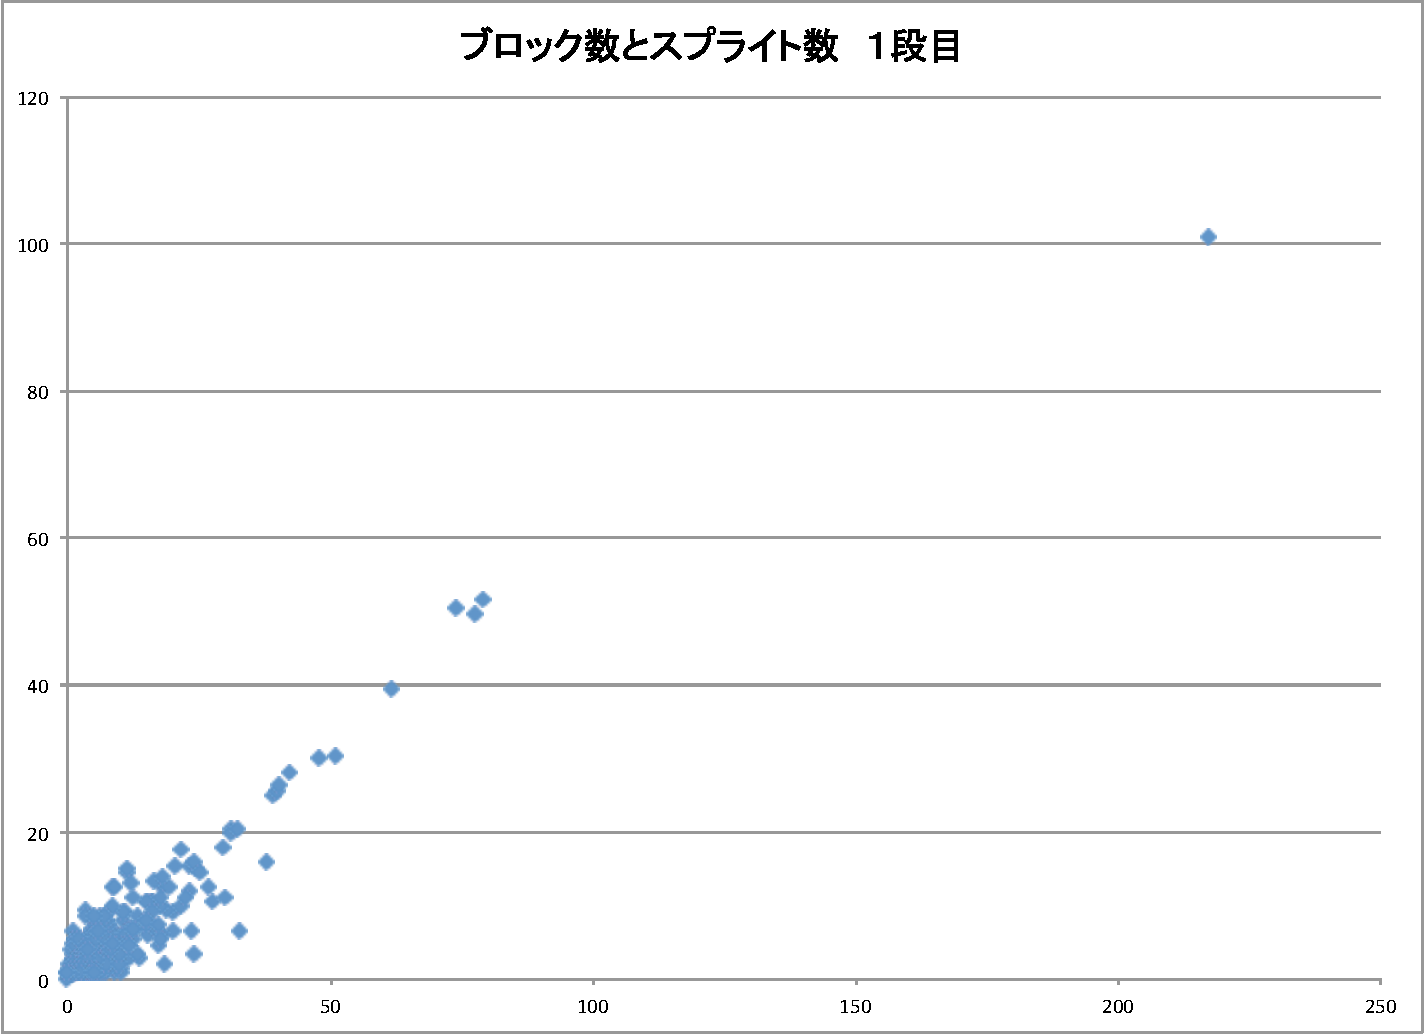
\includegraphics[keepaspectratio, scale = 0.25]{block_splite_1.pdf}
	 \caption{1段目のグラフ}
	 \label{first_block_splite}
	\end{minipage}
        \begin{minipage}[t]{0.45\hsize}
	 \centering
	 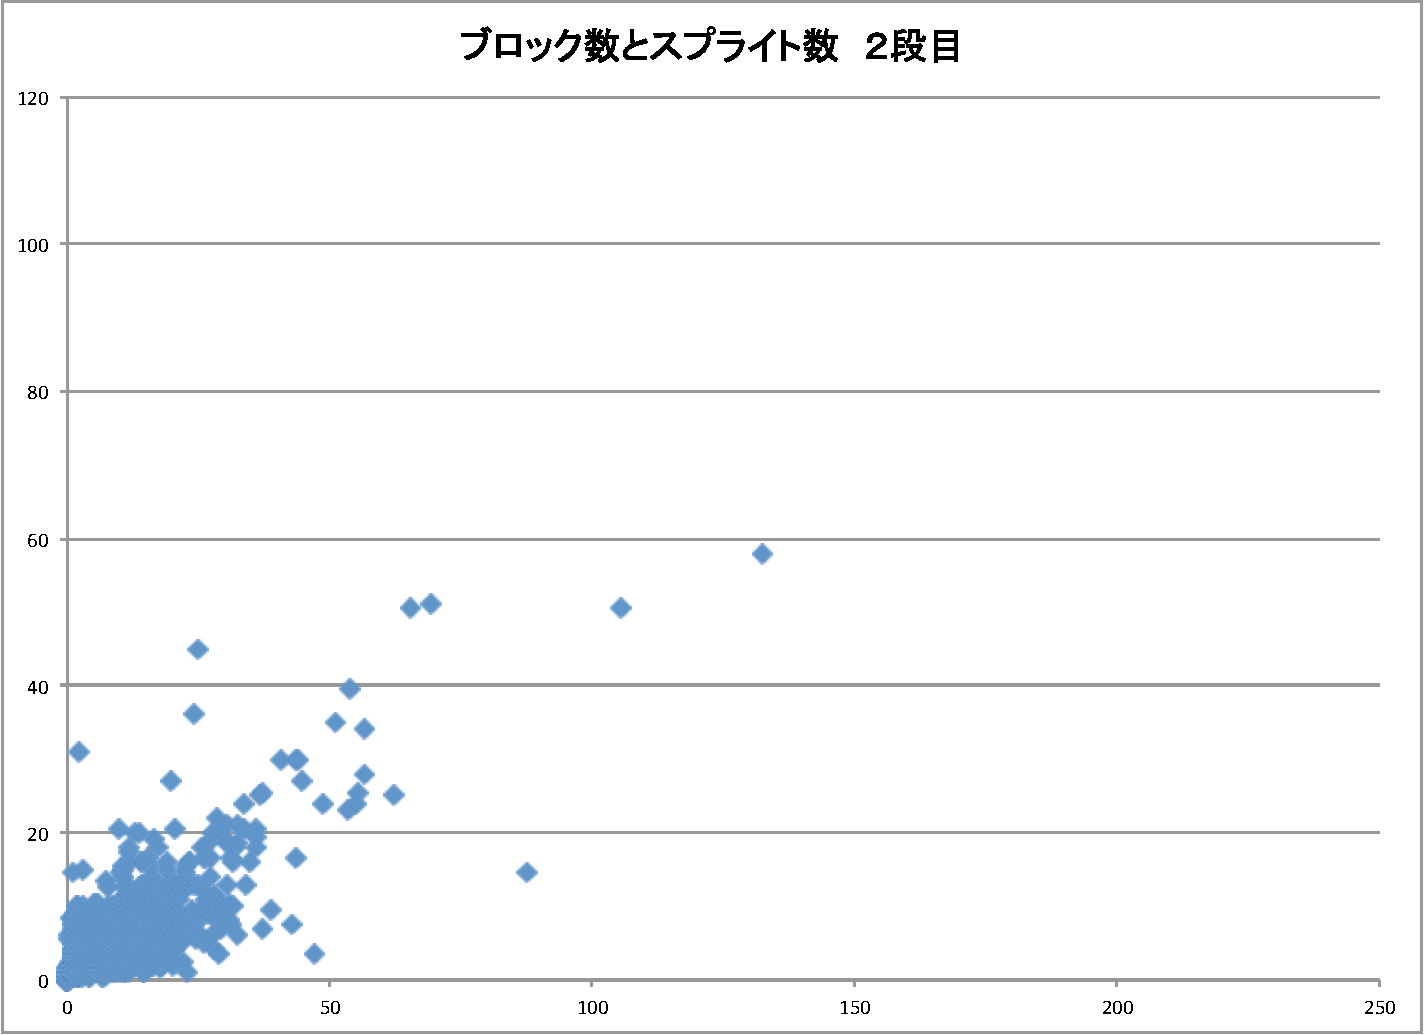
\includegraphics[keepaspectratio, scale = 0.25]{block_splite_2.pdf}
	 \caption{2段目のグラフ}
	 \label{second_block_splite}
	\end{minipage}
 \end{tabular}
  \begin{tabular}{cc}
 	\begin{minipage}[t]{0.45\hsize}
	 \centering
	 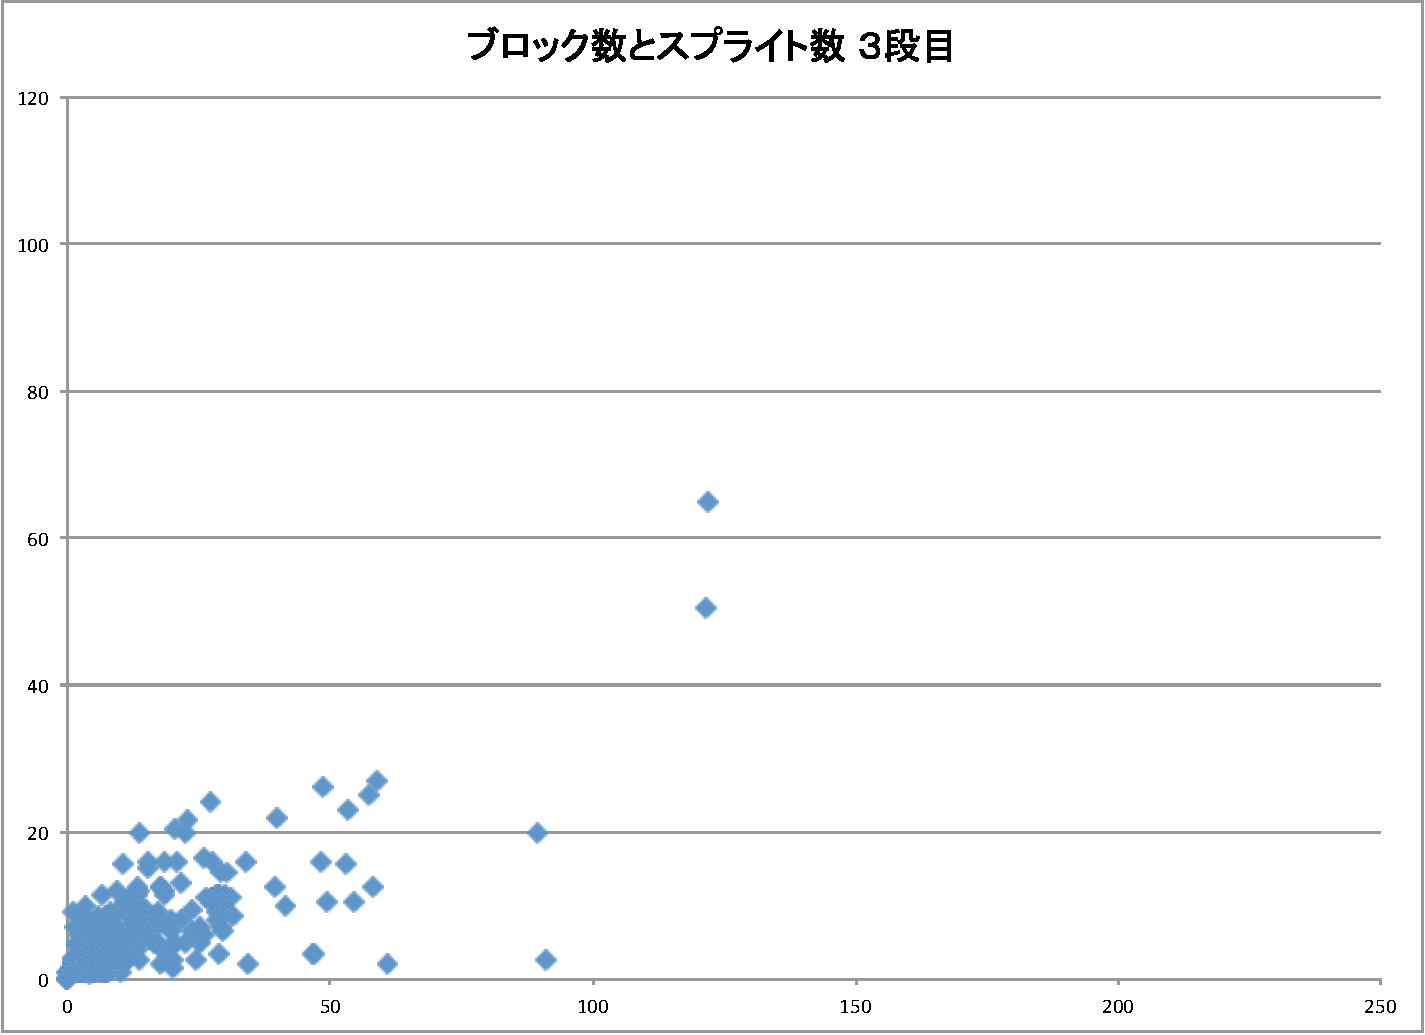
\includegraphics[keepaspectratio, scale = 0.25]{block_splite_3.pdf}
	 \caption{3段目のグラフ}
	 \label{third_block_splite}
	\end{minipage}
        \begin{minipage}[t]{0.45\hsize}
	 \centering
	 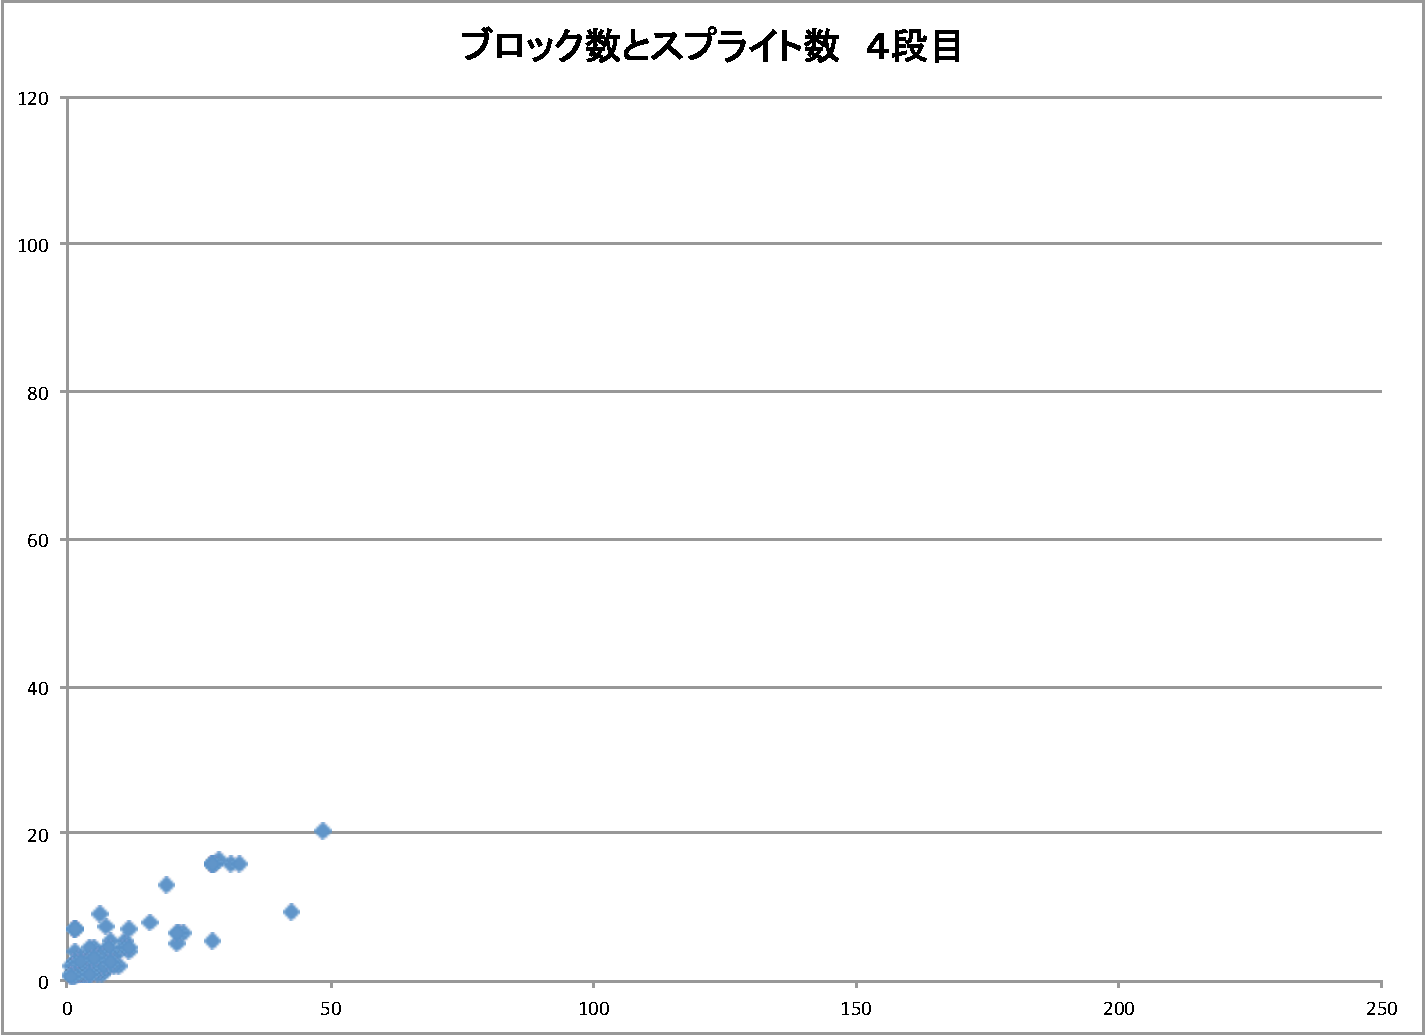
\includegraphics[keepaspectratio, scale = 0.25]{block_splite_4.pdf}
	 \caption{4段目のグラフ}
	 \label{fourth_block_splite}
	\end{minipage}
 \end{tabular}
 \end{figure}

\newpage
 \subsection{スプライト数あたりのブロック数とcos類似度の散布図}
出力されたデータを元にブロック数をスプライト数で割り、その値とcos類似度の散布図を作成した。4つの比較ができるように、目盛りは全ての最大値に揃えた。

\begin{figure}[h]
 \begin{tabular}{cc}
 	\begin{minipage}[t]{0.45\hsize}
	 \centering
	 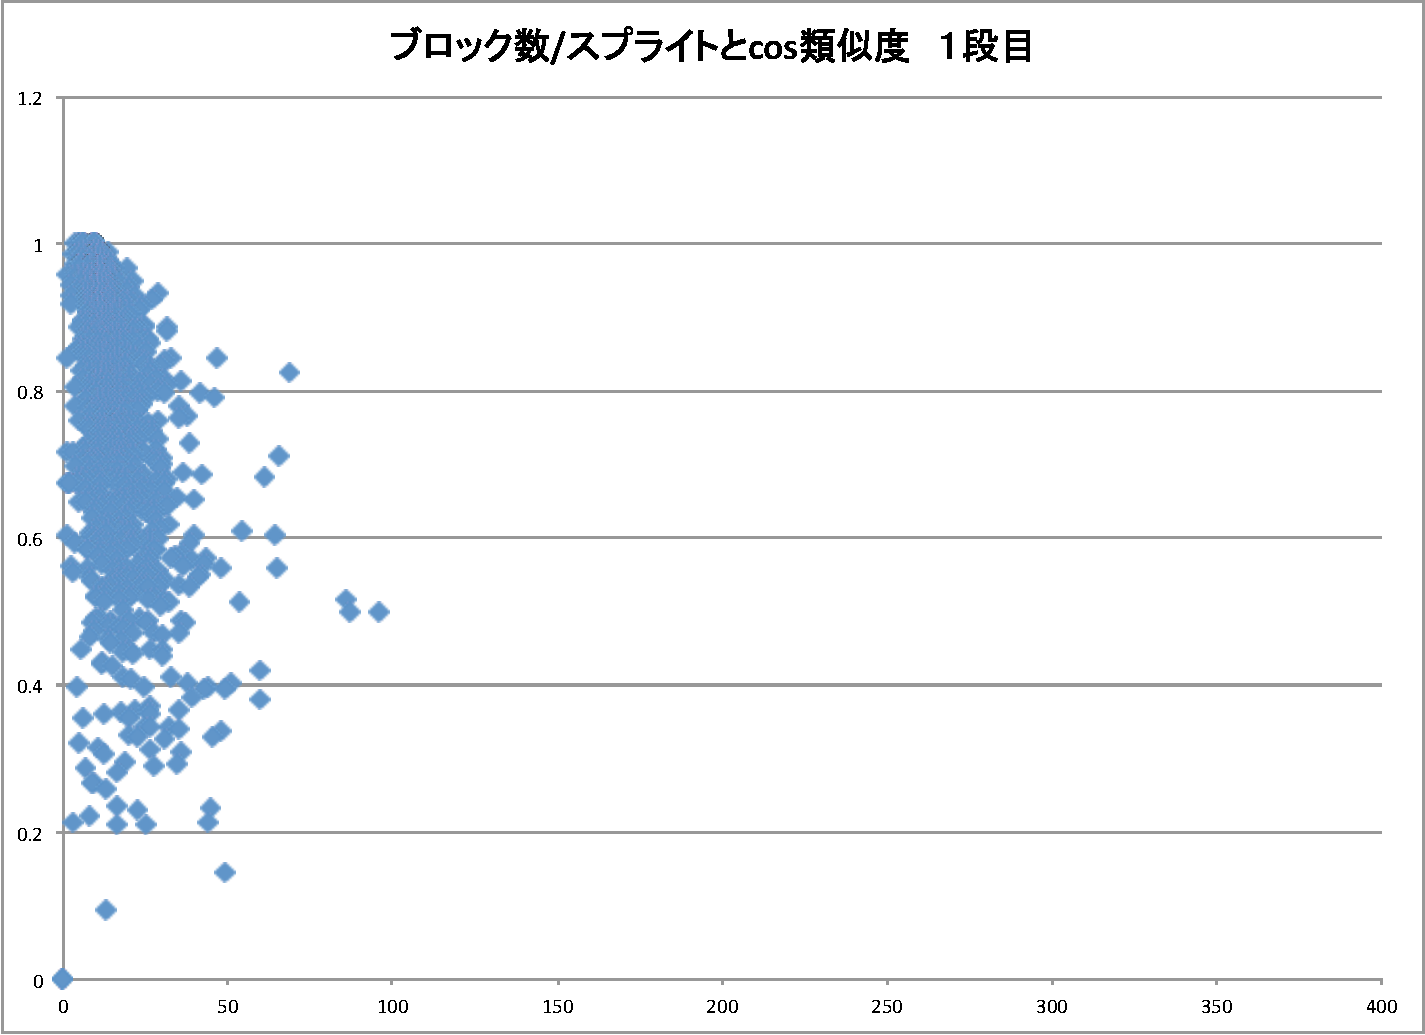
\includegraphics[keepaspectratio, scale = 0.25]{block_per_splite_1.pdf}
	 \caption{1段目のグラフ}
	 \label{first_block_per_splite}
	\end{minipage}
        \begin{minipage}[t]{0.45\hsize}
	 \centering
	 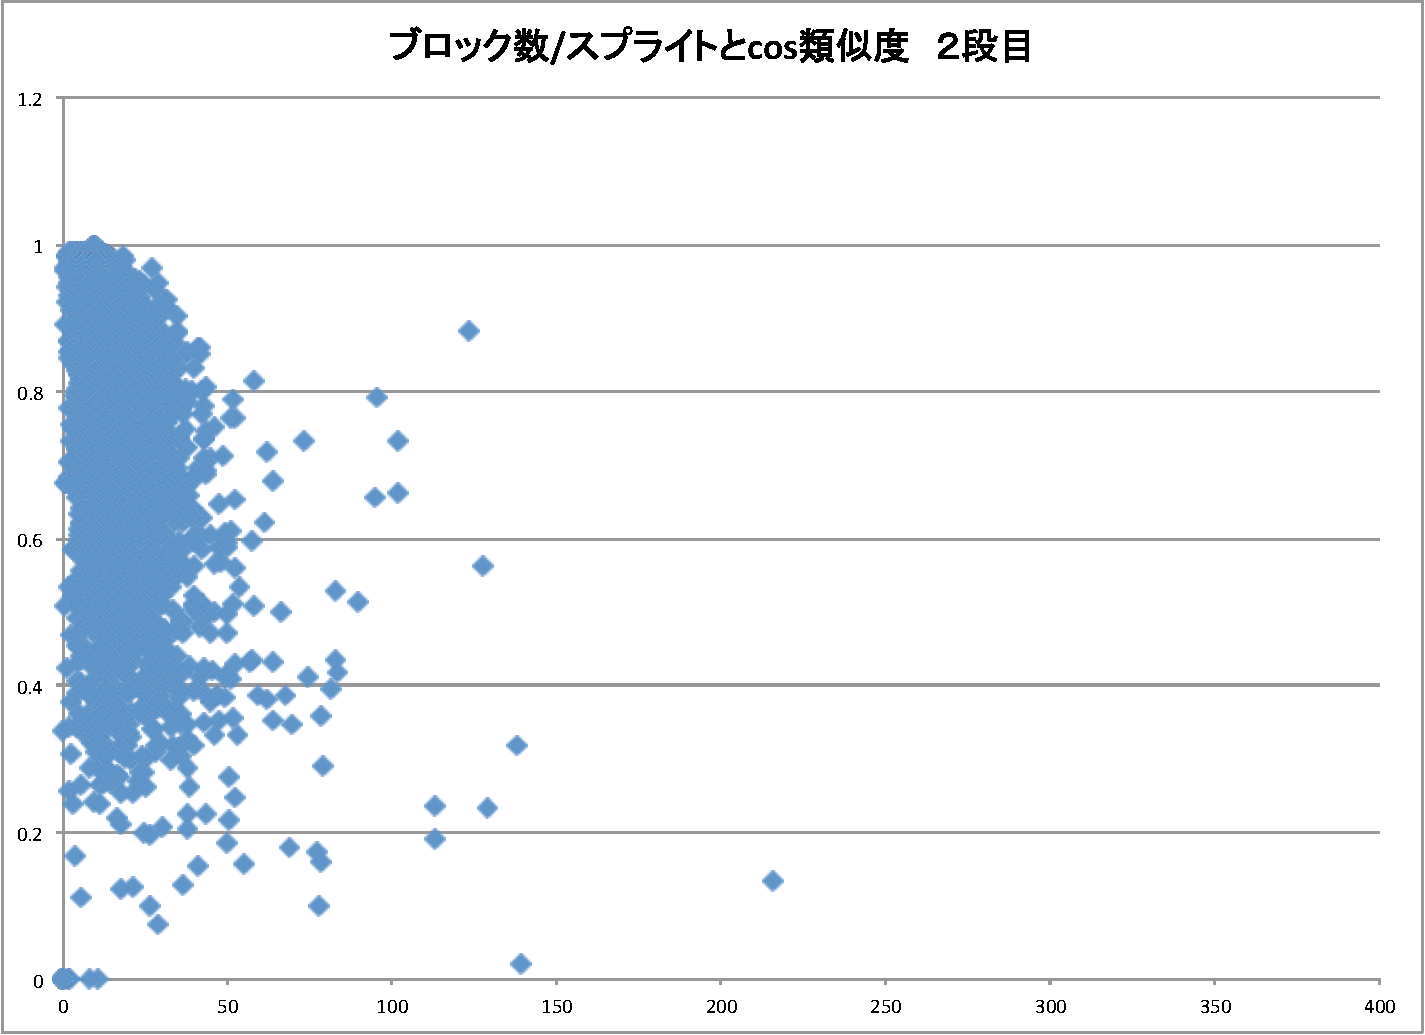
\includegraphics[keepaspectratio, scale = 0.25]{block_per_splite_2.pdf}
	 \caption{2段目のグラフ}
	 \label{second_block_per_splite}
	\end{minipage}
 \end{tabular}
  \begin{tabular}{cc}
 	\begin{minipage}[t]{0.45\hsize}
	 \centering
	 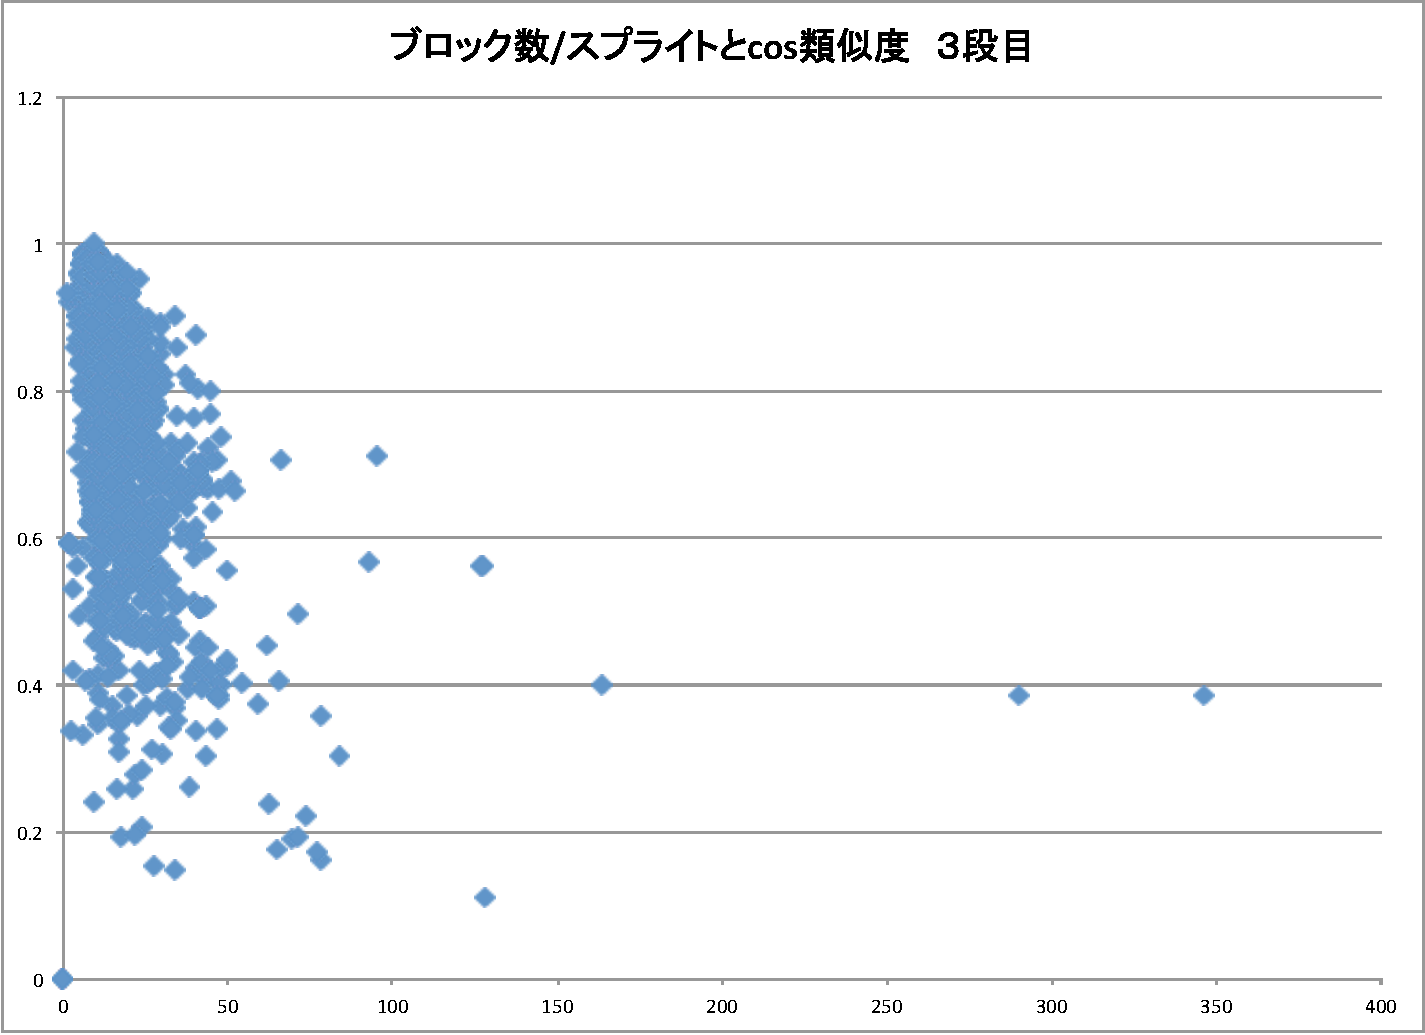
\includegraphics[keepaspectratio, scale = 0.25]{block_per_splite_3.pdf}
	 \caption{3段目のグラフ}
	 \label{third_block_per_splite}
	\end{minipage}
        \begin{minipage}[t]{0.45\hsize}
	 \centering
	 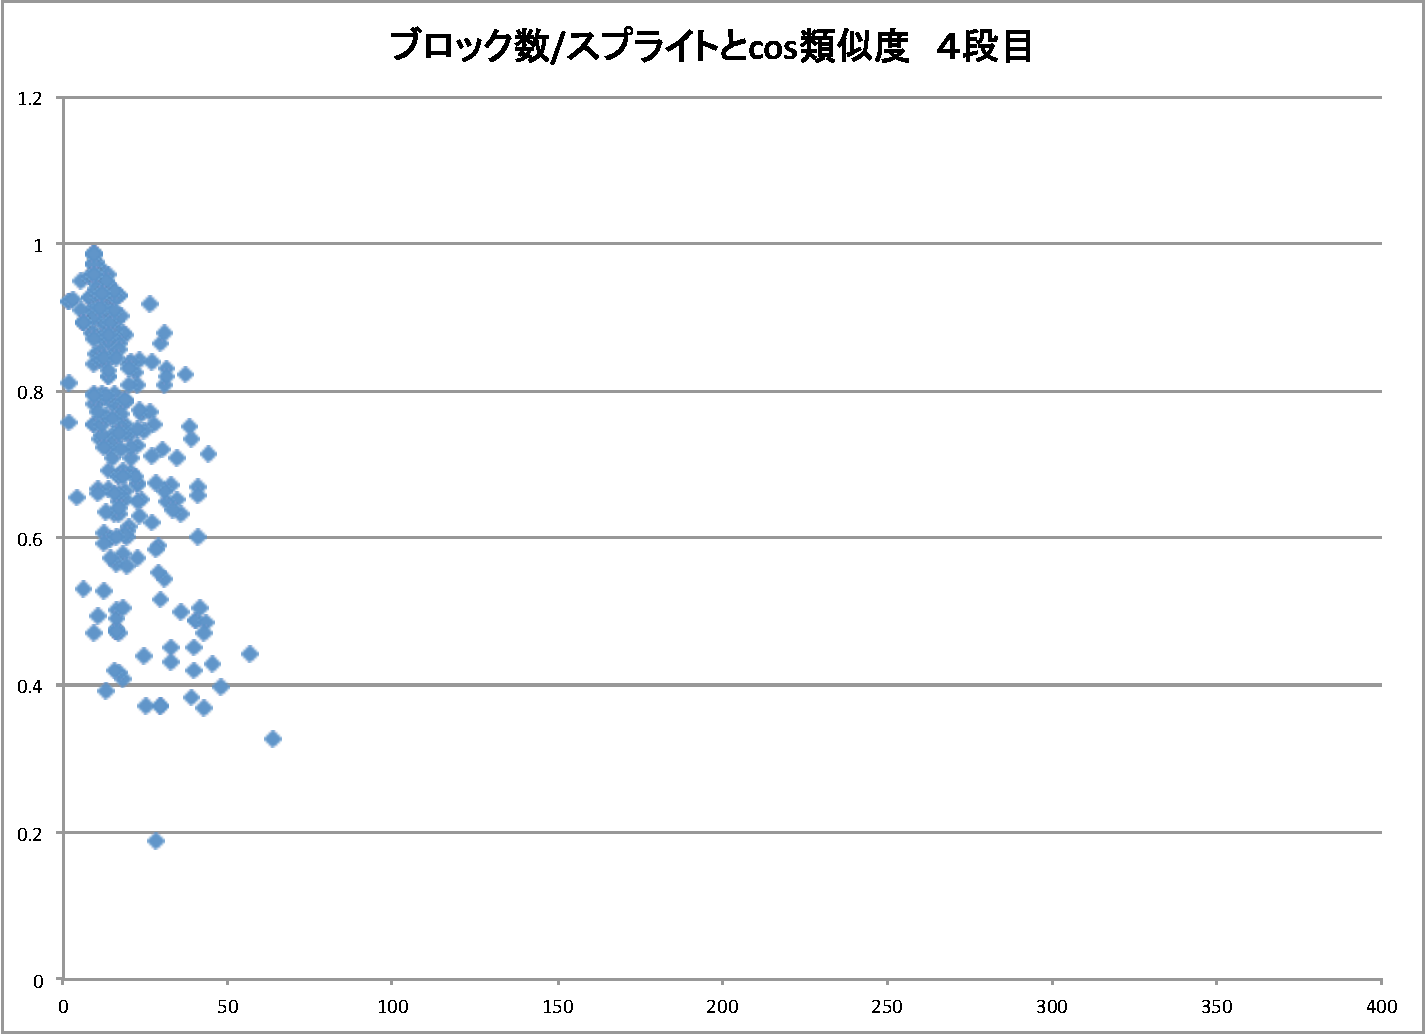
\includegraphics[keepaspectratio, scale = 0.25]{block_per_splite_4.pdf}
	 \caption{4段目のグラフ}
	 \label{fourth_block_per_splite}
	\end{minipage}
 \end{tabular}
 \end{figure}

\newpage
\subsection{ブロック数とcos類似度の散布図}
 出力されたデータを元に横軸がブロック数、縦軸がcos類似度の散布図を作成した。ブロック数は19で割ったあと10の対数を目盛りにした。4つの比較ができるように、目盛りは全ての最大値に揃えた。

\begin{figure}[h]
 \begin{tabular}{cc}
 	\begin{minipage}[t]{0.45\hsize}
	 \centering
	 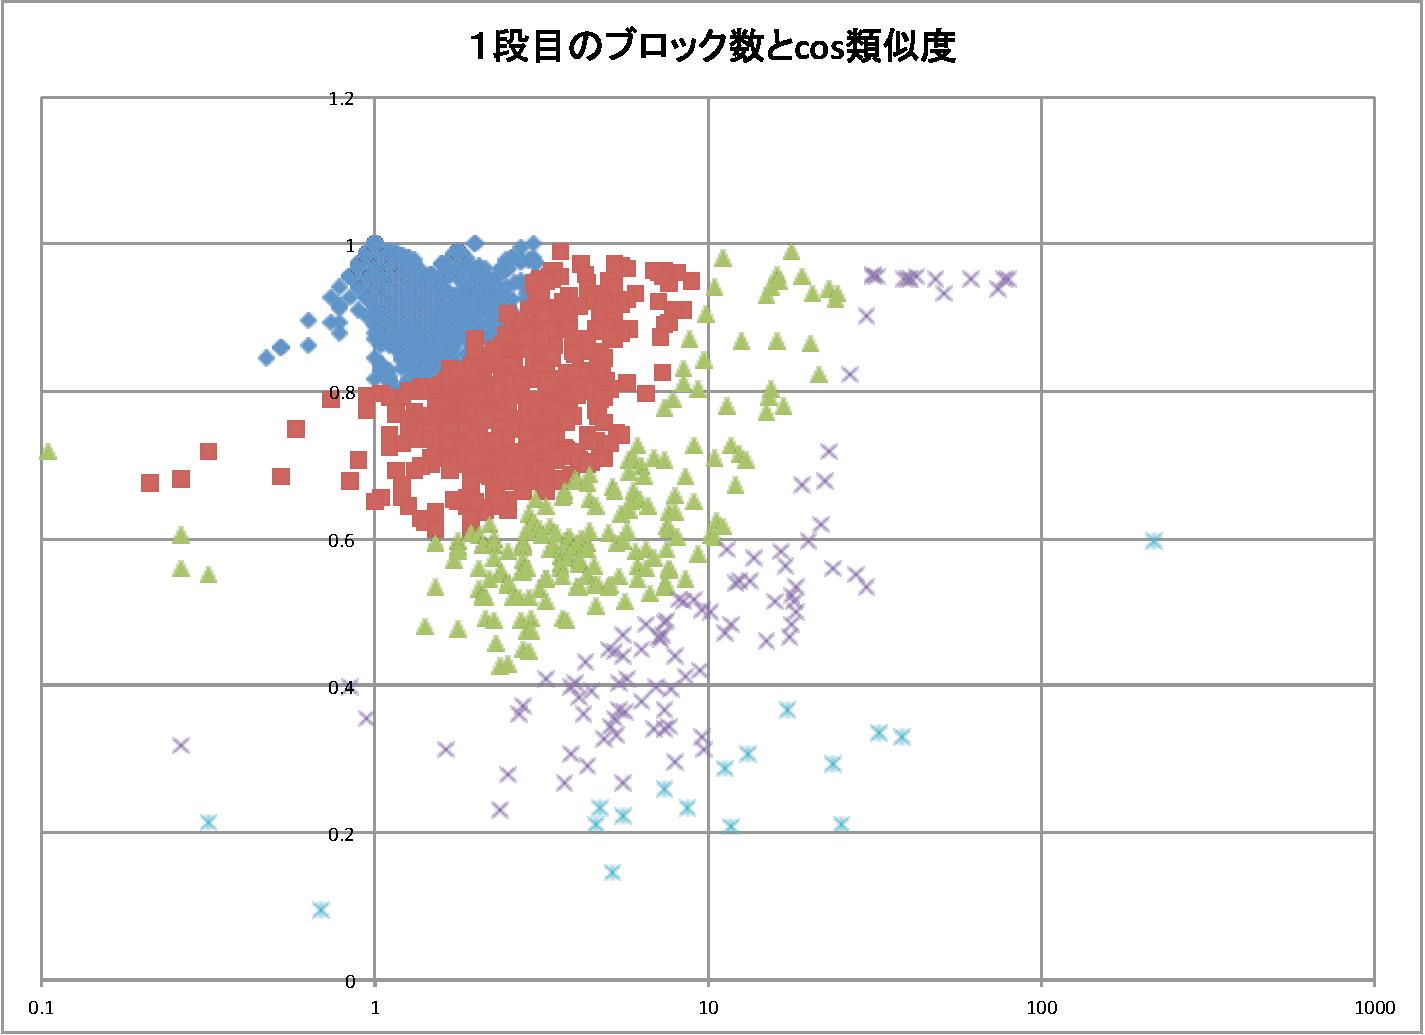
\includegraphics[keepaspectratio, scale = 0.25]{graph_1_block.pdf}
	 \caption{1段目のグラフ}
	 \label{first_block_cos}
	\end{minipage}
        \begin{minipage}[t]{0.45\hsize}
	 \centering
	 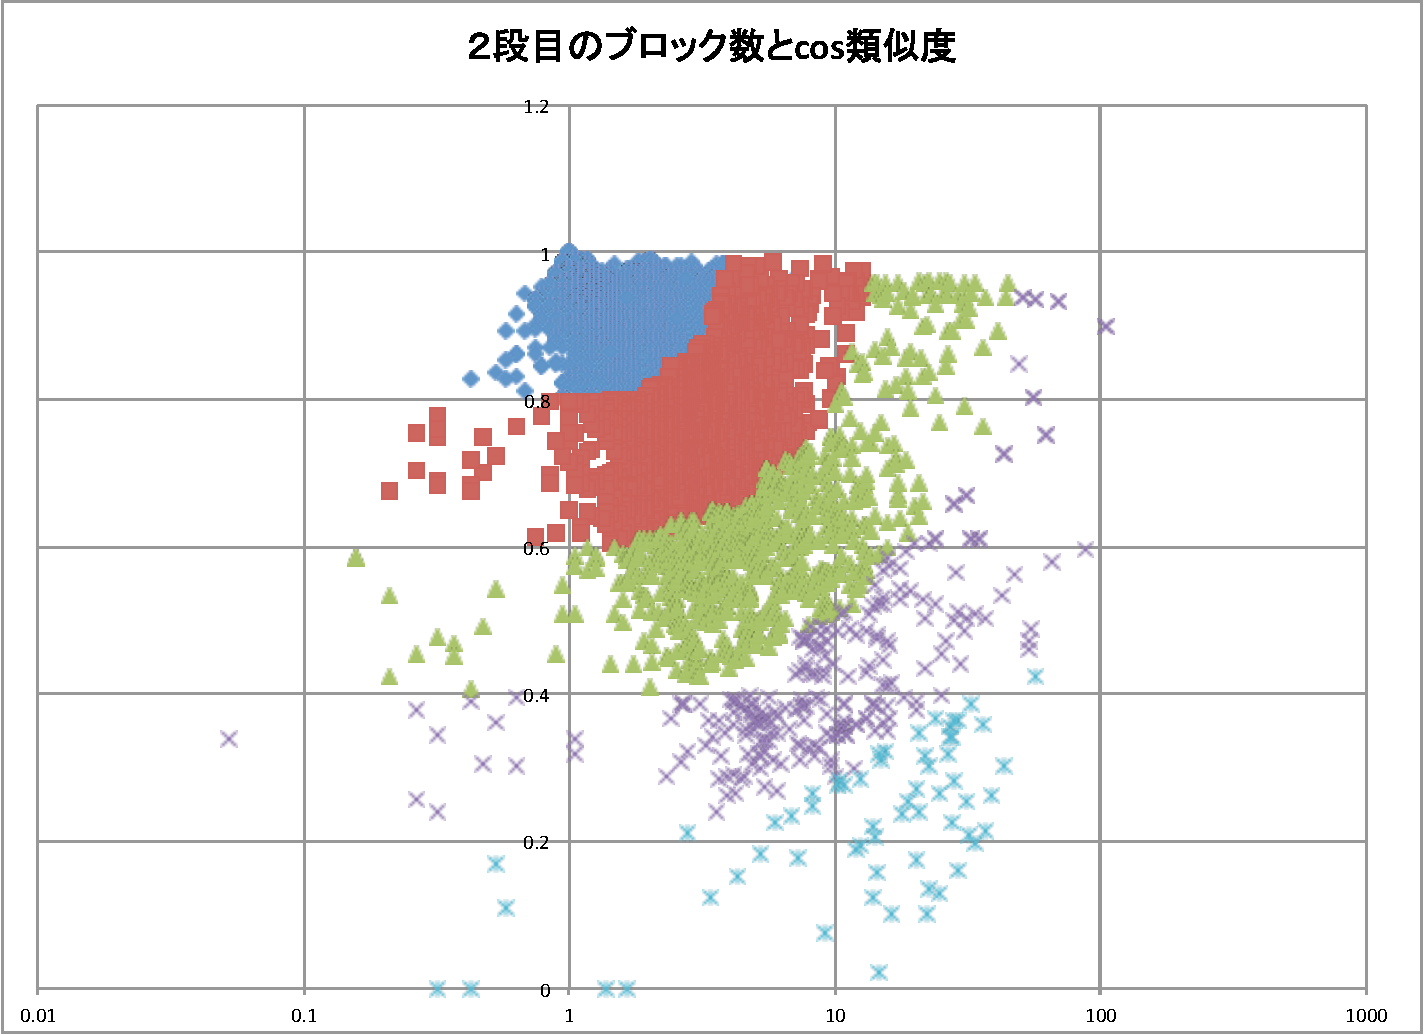
\includegraphics[keepaspectratio, scale = 0.25]{graph_2_block.pdf}
	 \caption{2段目のグラフ}
	 \label{second_block_cos}
	\end{minipage}
 \end{tabular}
  \begin{tabular}{cc}
 	\begin{minipage}[t]{0.45\hsize}
	 \centering
	 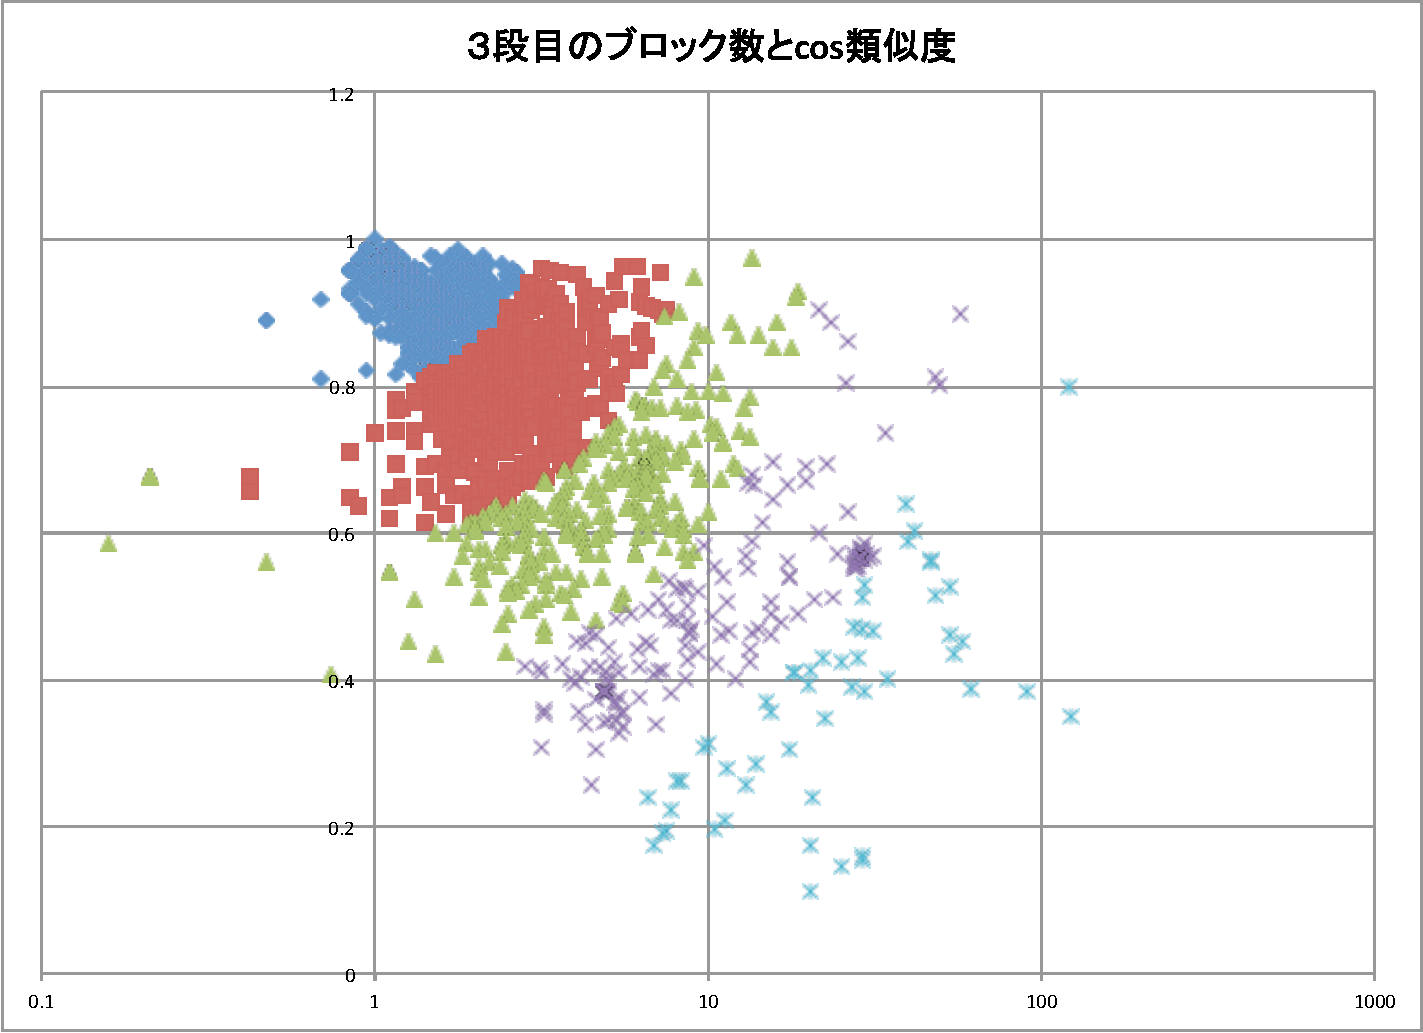
\includegraphics[keepaspectratio, scale = 0.25]{graph_3_block.pdf}
	 \caption{3段目のグラフ}
	 \label{third_block_cos}
	\end{minipage}
        \begin{minipage}[t]{0.45\hsize}
	 \centering
	 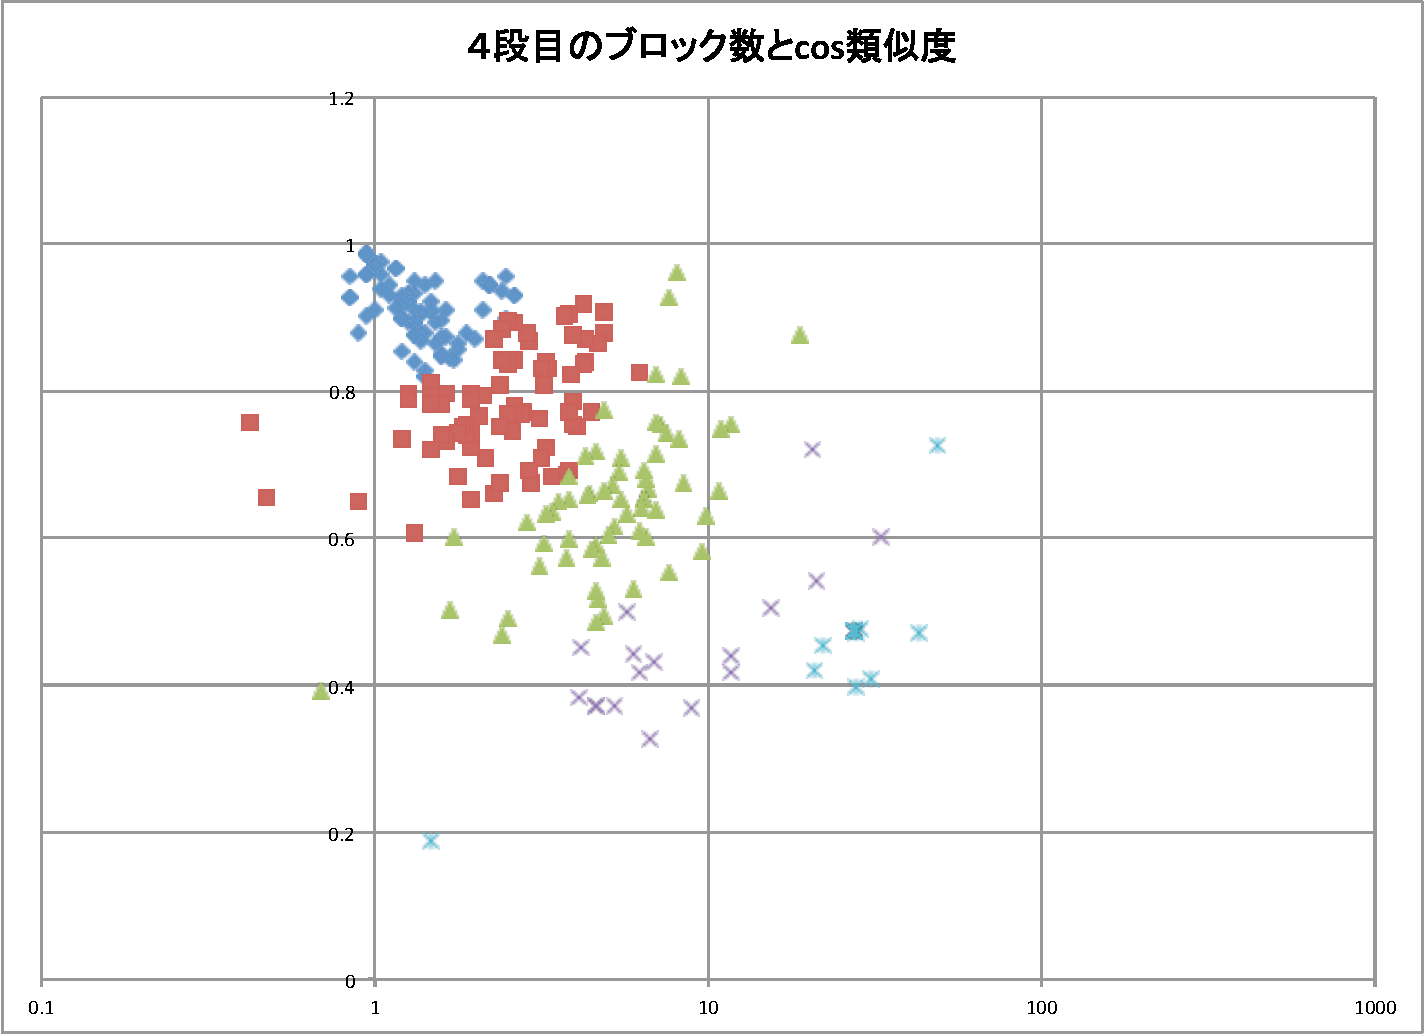
\includegraphics[keepaspectratio, scale = 0.25]{graph_4_block.pdf}
	 \caption{4段目のグラフ}
	 \label{fourth_block_cos}
	\end{minipage}
 \end{tabular}
 \end{figure}

\newpage
\subsection{スプライト数とcos類似度の散布図}
 出力されたデータを元に横軸がスプライト数、縦軸がcos類似度の散布図を作成した。ブロック数は2で割ったあと10の対数を目盛りにした。4つの比較ができるように、目盛りは全ての最大値に揃えた。

\begin{figure}[h]
 \begin{tabular}{cc}
 	\begin{minipage}[t]{0.45\hsize}
	 \centering
	 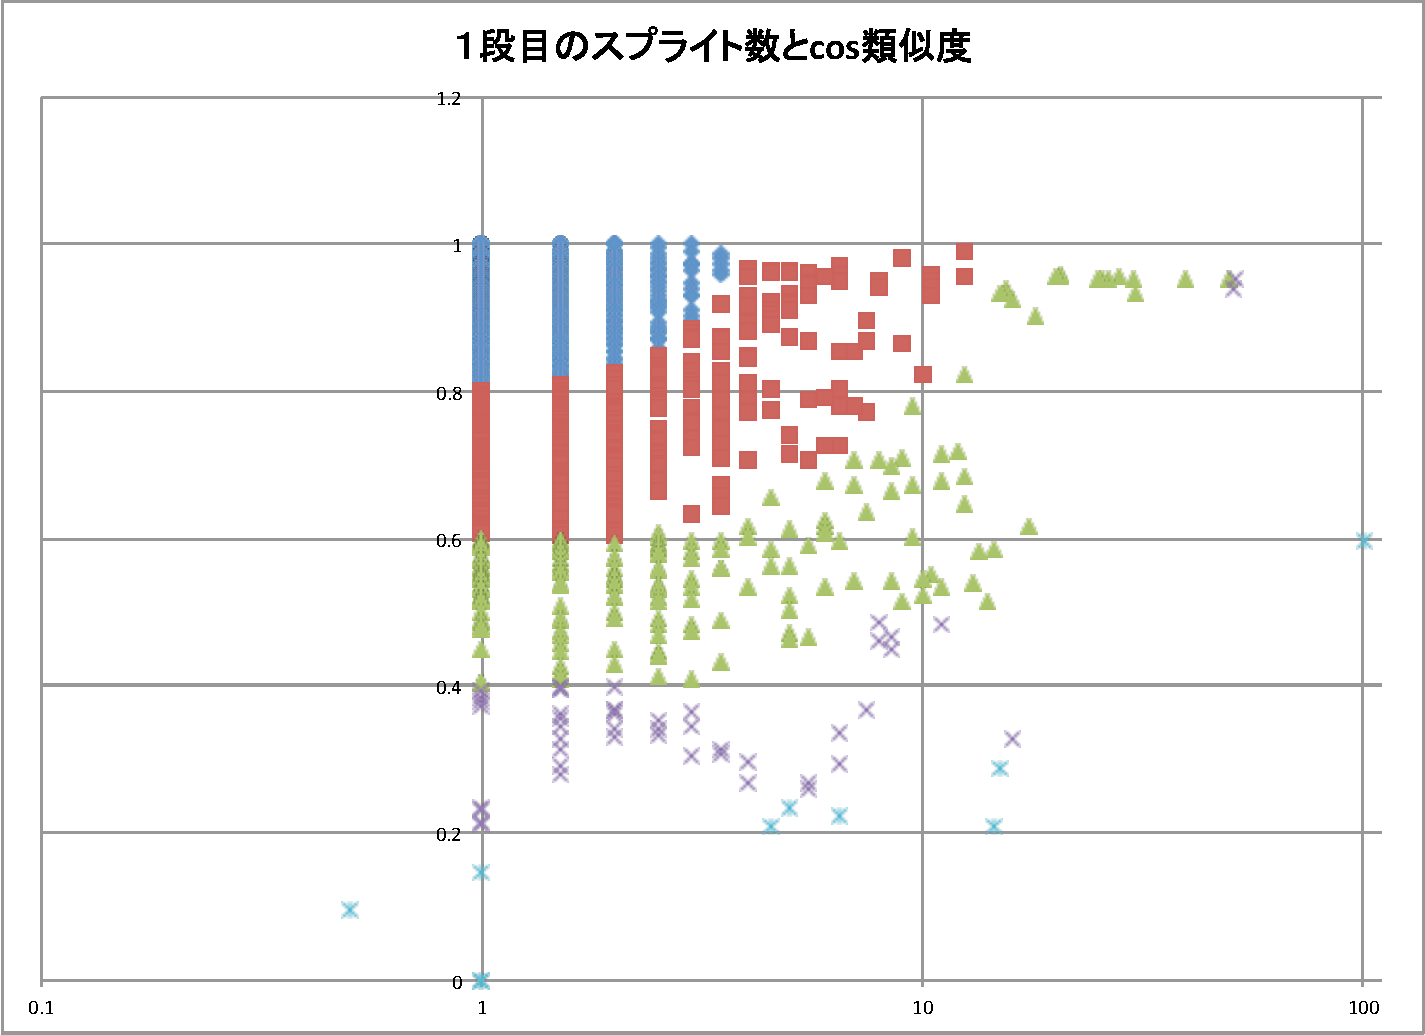
\includegraphics[keepaspectratio, scale = 0.25]{graph_1_splite.pdf}
	 \caption{1段目のグラフ}
	 \label{first_splite_cos}
	\end{minipage}
        \begin{minipage}[t]{0.45\hsize}
	 \centering
	 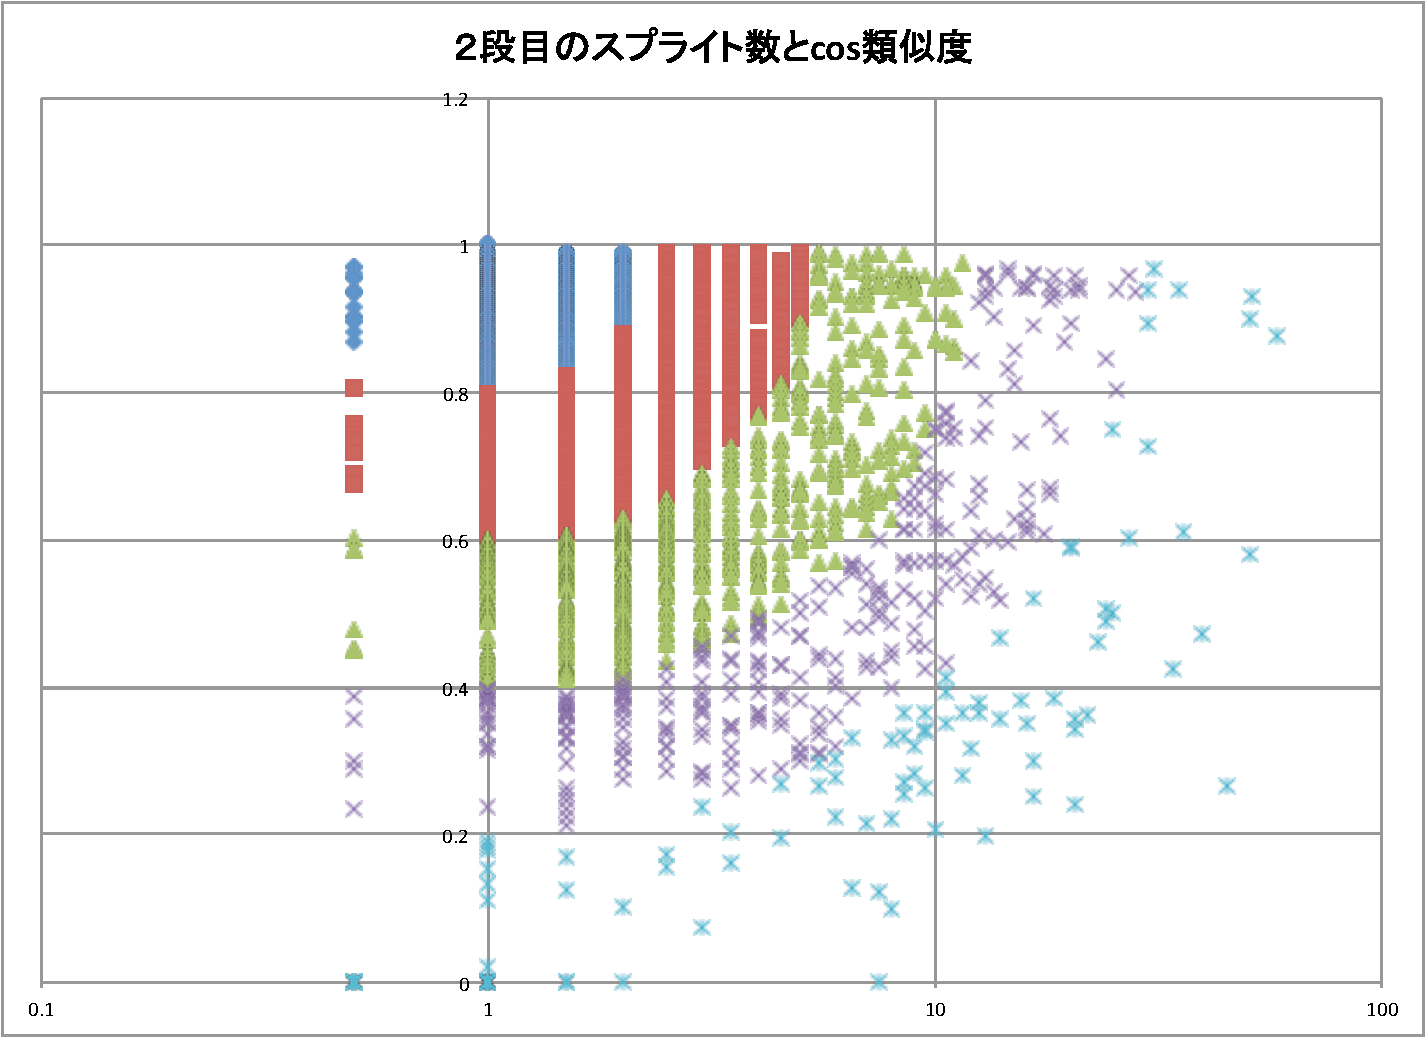
\includegraphics[keepaspectratio, scale = 0.25]{graph_2_splite.pdf}
	 \caption{2段目のグラフ}
	 \label{second_splite_cos}
	\end{minipage}
 \end{tabular}
  \begin{tabular}{cc}
 	\begin{minipage}[t]{0.45\hsize}
	 \centering
	 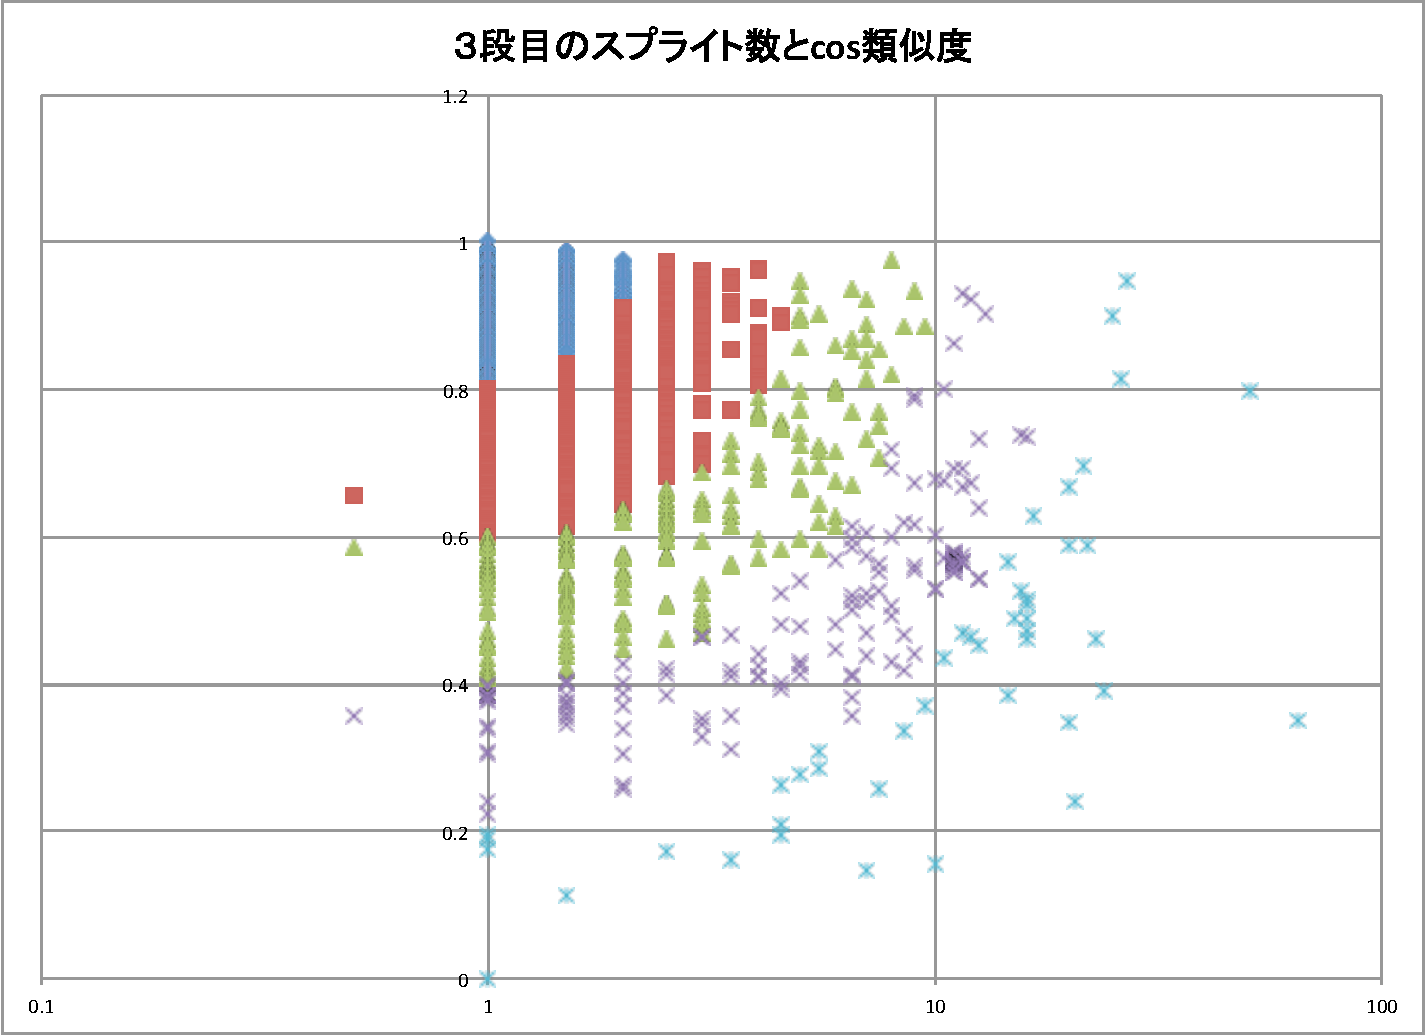
\includegraphics[keepaspectratio, scale = 0.25]{graph_3_splite.pdf}
	 \caption{3段目のグラフ}
	 \label{third_splite_cos}
	\end{minipage}
        \begin{minipage}[t]{0.45\hsize}
	 \centering
	 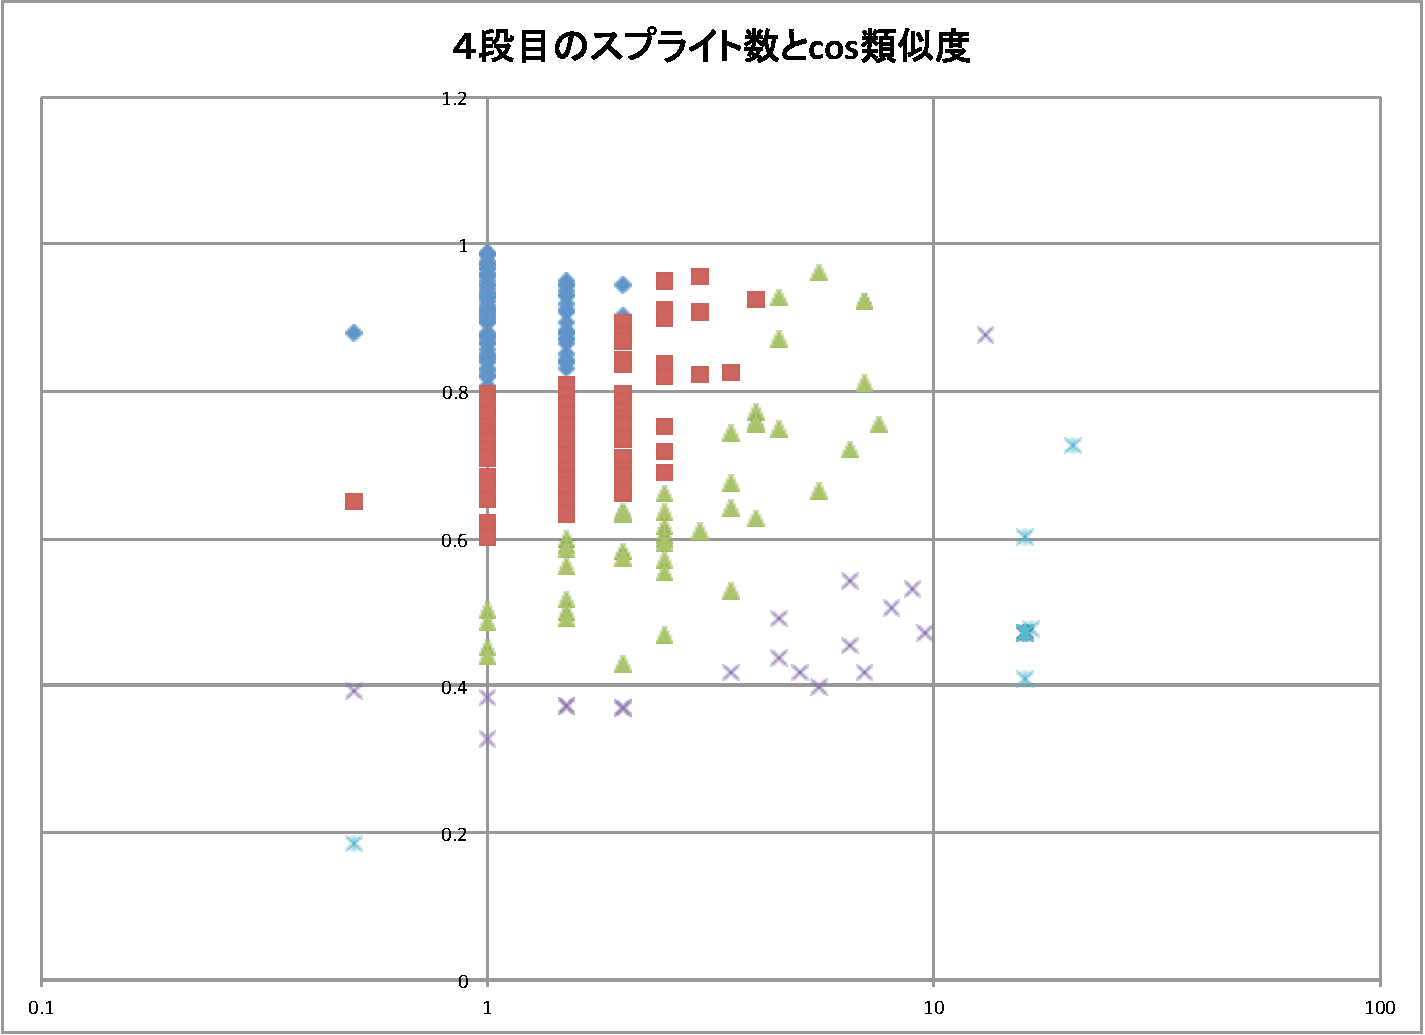
\includegraphics[keepaspectratio, scale = 0.25]{graph_4_splite.pdf}
	 \caption{4段目のグラフ}
	 \label{fourth_splite_cos}
	\end{minipage}
 \end{tabular}
 \end{figure}
 
\newpage
\subsection{ブロック数とcos類似度の個数によるカラープロット}
出力されたデータを元に同じデータの個数の集計を行い、その個数を色の濃淡で表した。ブロック数は19で割り、4つのグラフを比較するため、目盛り数を最大値に揃えた。

\begin{figure}[h]
 \begin{tabular}{cc}
 	\begin{minipage}[t]{0.45\hsize}
	 \centering
	 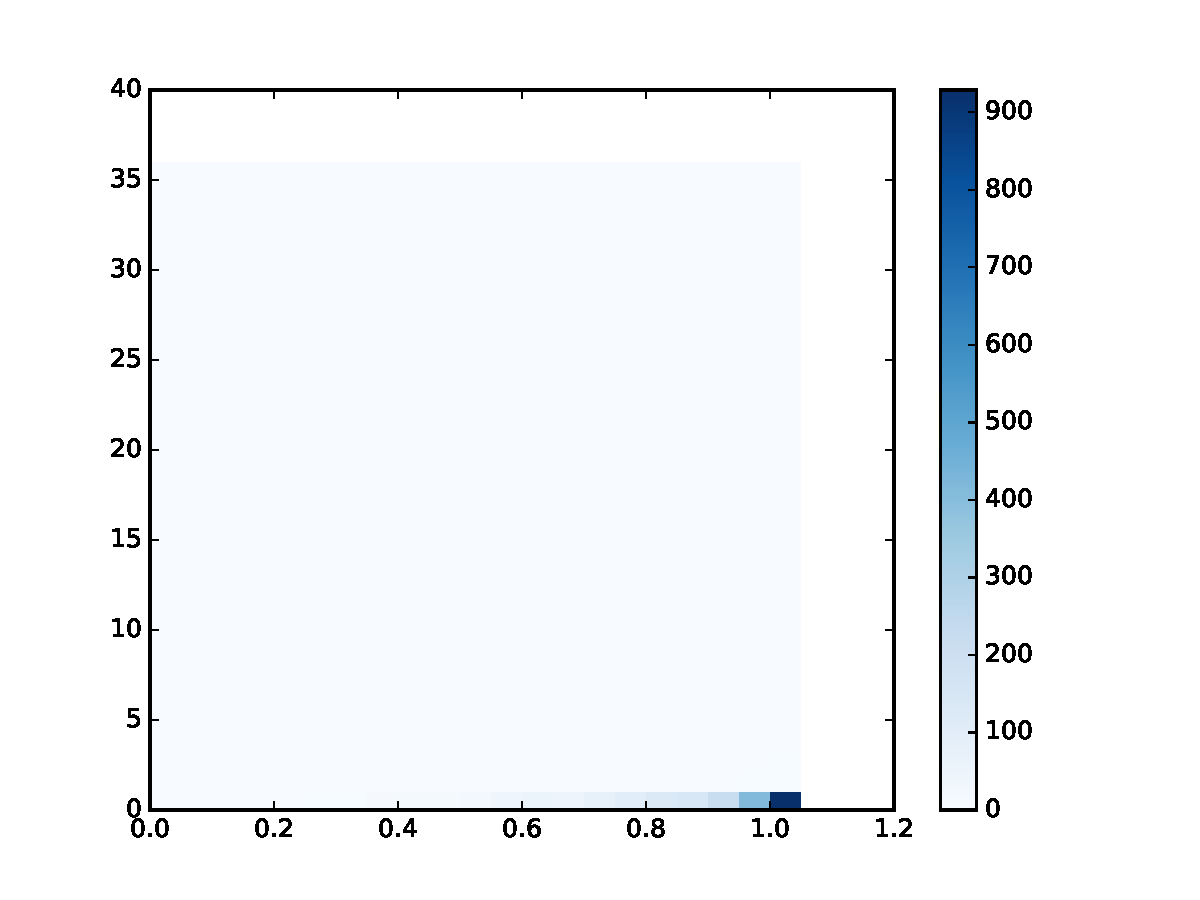
\includegraphics[keepaspectratio, scale = 0.35]{colormap_block_1.pdf}
	 \caption{1段目のグラフ}
	 \label{first_block_color}
	\end{minipage}
        \begin{minipage}[t]{0.45\hsize}
	 \centering
	 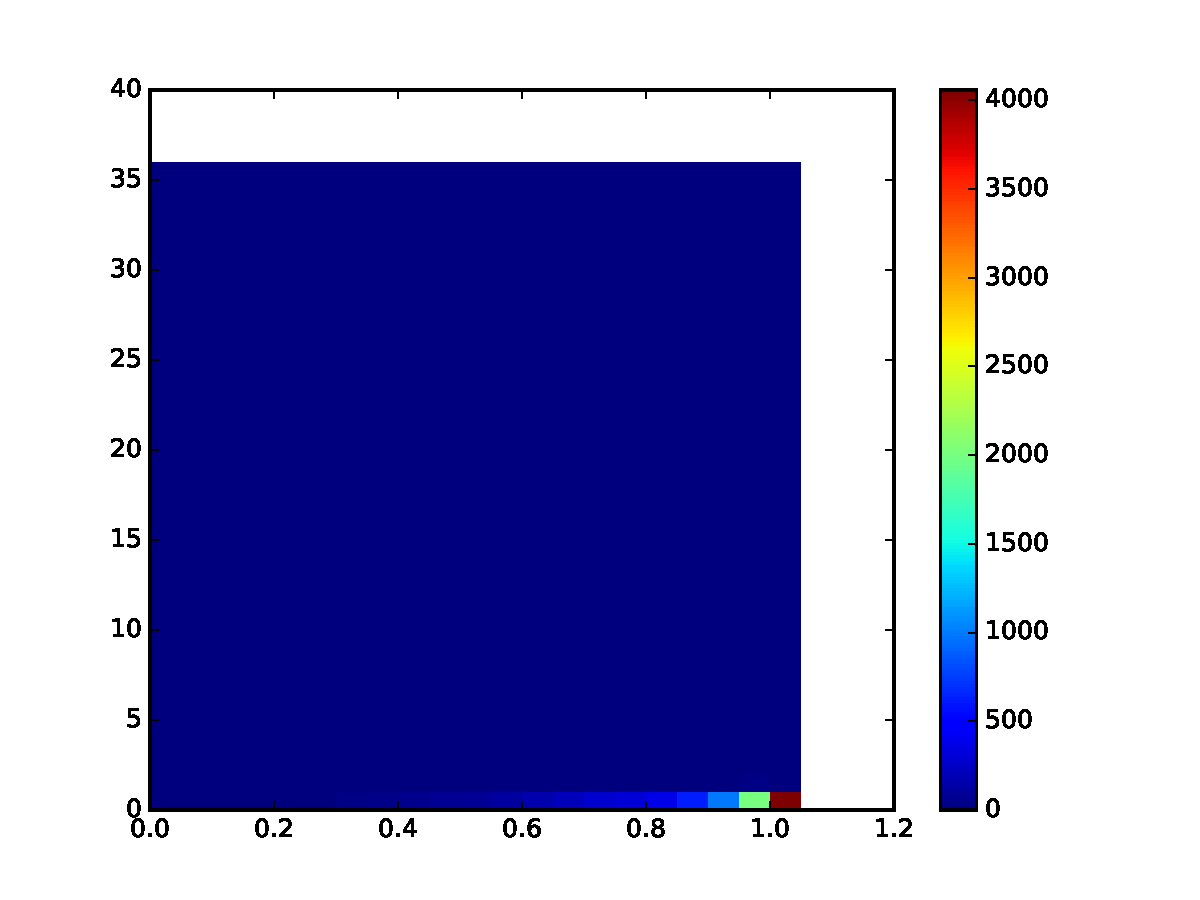
\includegraphics[keepaspectratio, scale = 0.35]{colormap_block_2.pdf}
	 \caption{2段目のグラフ}
	 \label{second_block_color}
	\end{minipage}
 \end{tabular}
  \begin{tabular}{cc}
 	\begin{minipage}[t]{0.45\hsize}
	 \centering
	 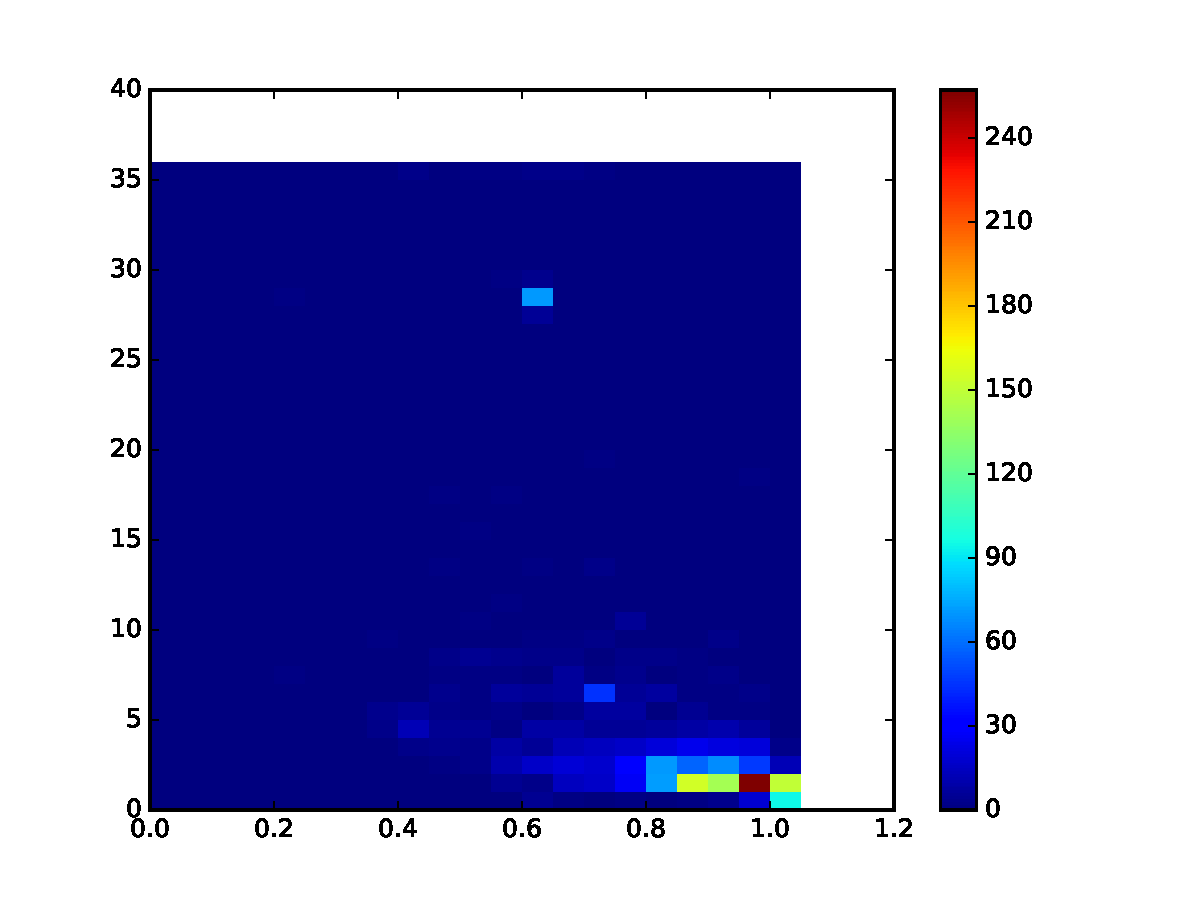
\includegraphics[keepaspectratio, scale = 0.35]{colormap_block_3.pdf}
	 \caption{3段目のグラフ}
	 \label{third_block_color}
	\end{minipage}
        \begin{minipage}[t]{0.45\hsize}
	 \centering
	 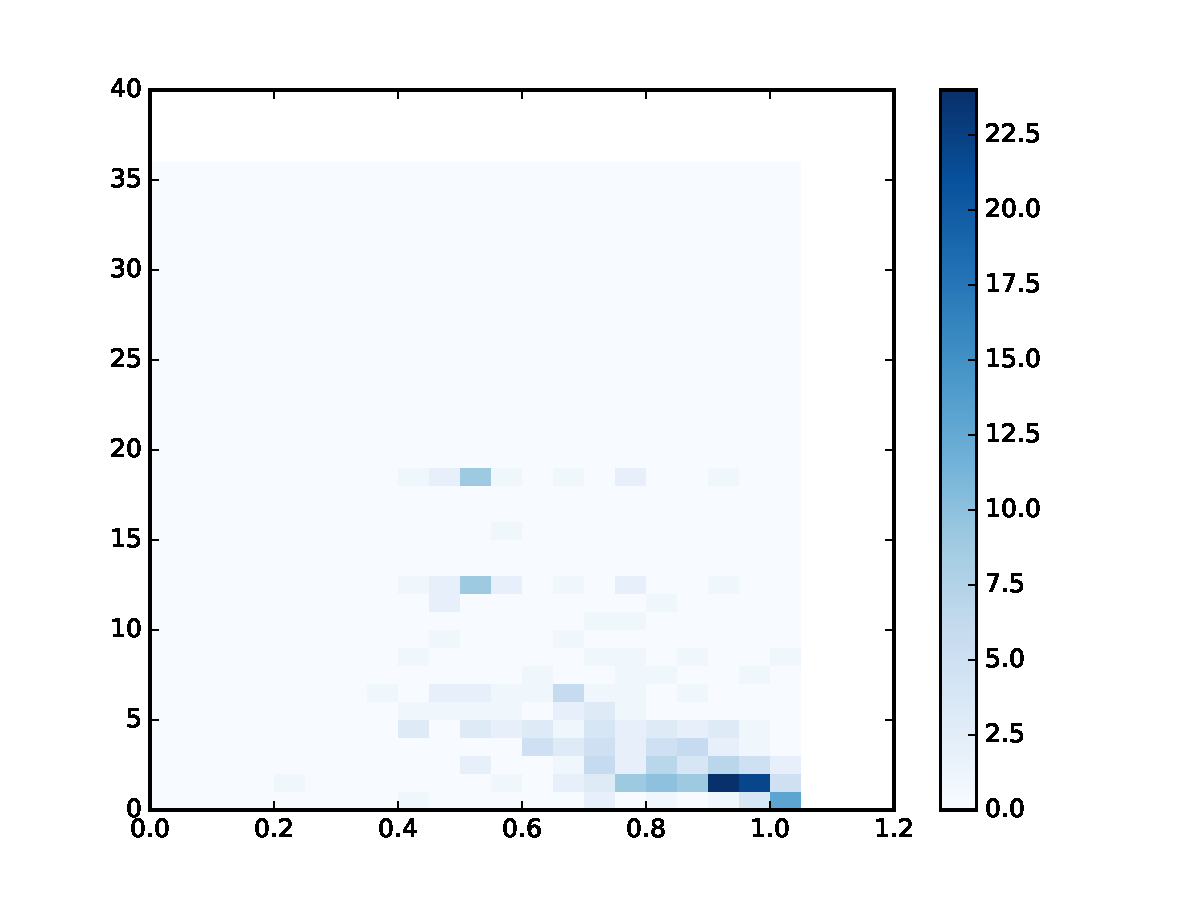
\includegraphics[keepaspectratio, scale = 0.35]{colormap_block_4.pdf}
	 \caption{4段目のグラフ}
	 \label{fourth_block_color}
	\end{minipage}
 \end{tabular}
 \end{figure}
  
\newpage
 \subsection{スプライト数とcos類似度の個数によるカラープロット}
出力されたデータを元に同じデータの個数の集計を行い、その個数を色の濃淡で表した。スプライト数は2で割り、4つのグラフを比較するため、目盛り数を最大値に揃えた。 
 
\begin{figure}[h]
 \begin{tabular}{cc}
 	\begin{minipage}[t]{0.45\hsize}
	 \centering
	 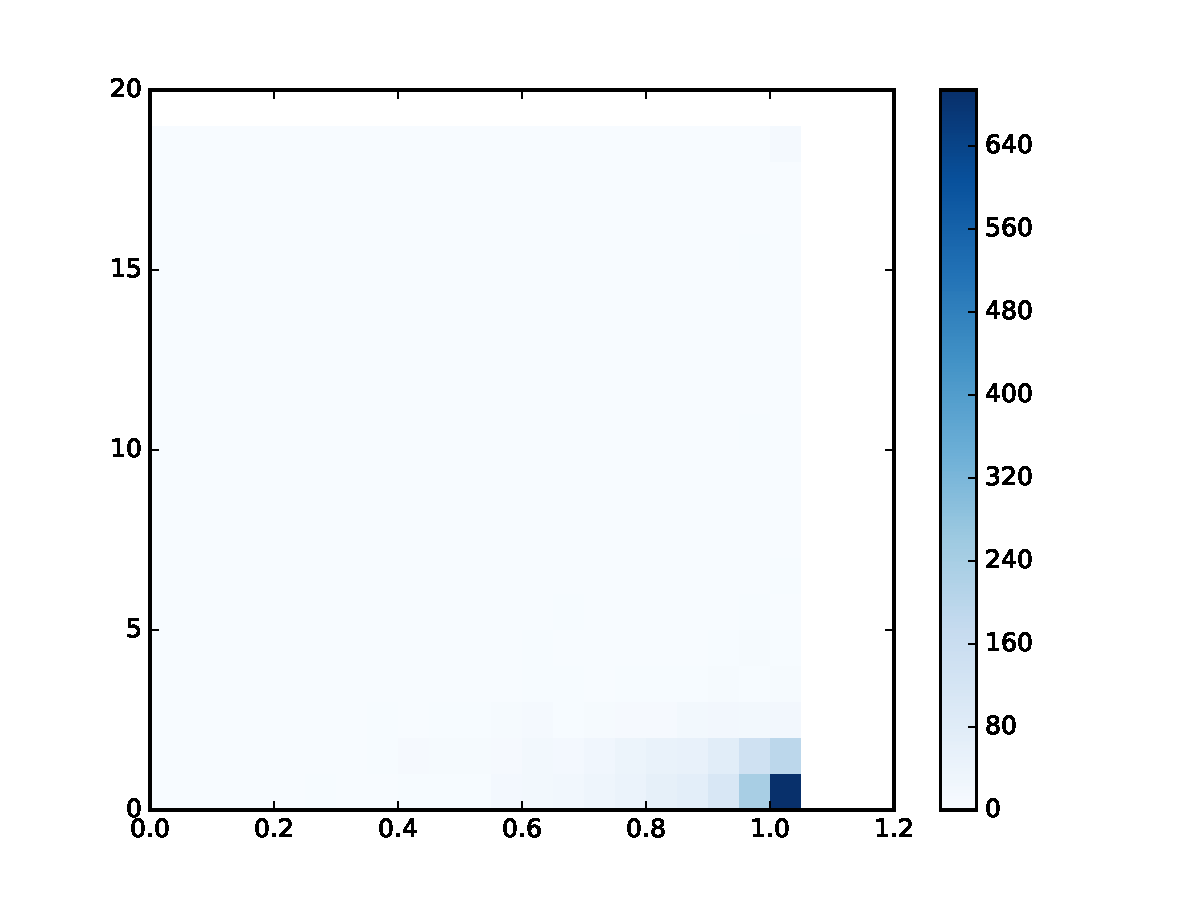
\includegraphics[keepaspectratio, scale = 0.35]{colormap_splite_1.pdf}
	 \caption{1段目のグラフ}
	 \label{first_splite_color}
	\end{minipage}
        \begin{minipage}[t]{0.45\hsize}
	 \centering
	 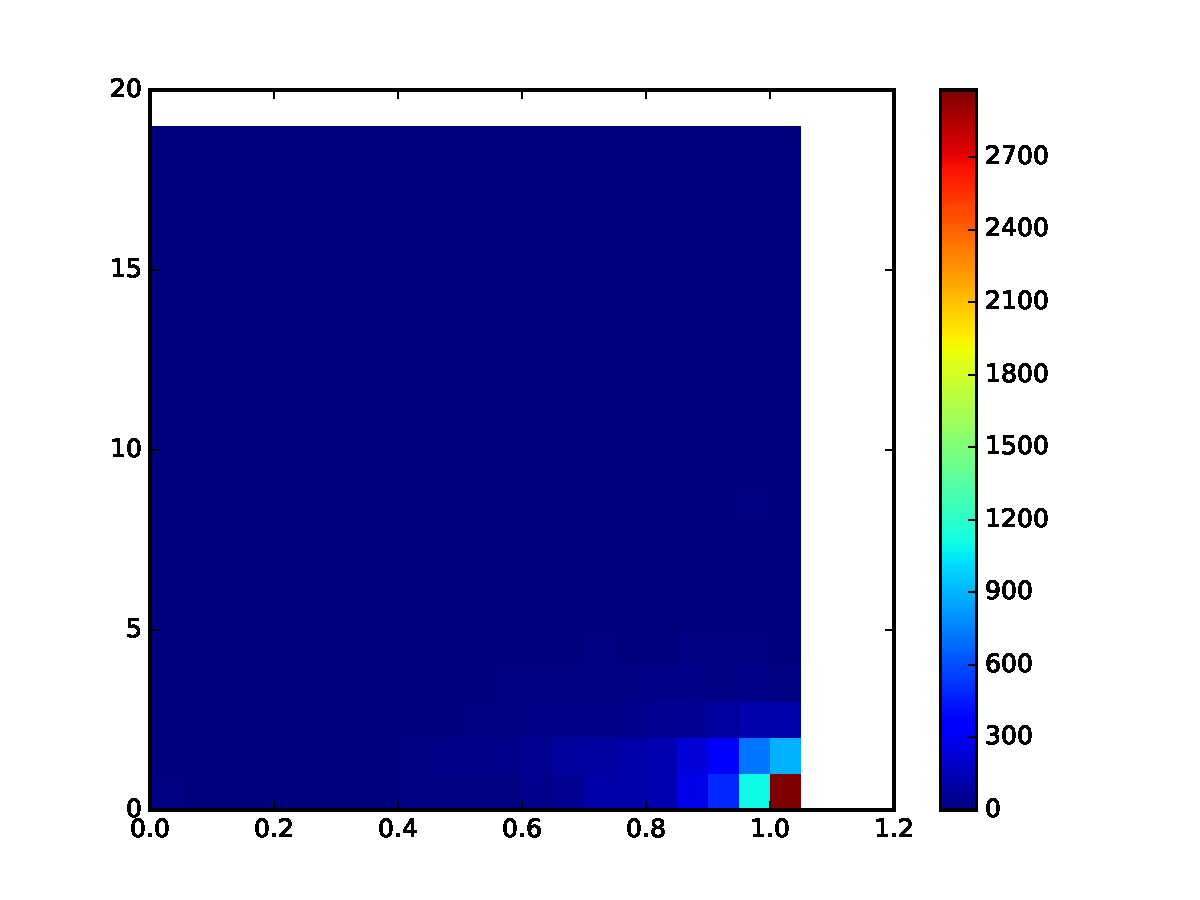
\includegraphics[keepaspectratio, scale = 0.35]{colormap_splite_2.pdf}
	 \caption{2段目のグラフ}
	 \label{second_splite_color}
	\end{minipage}
 \end{tabular}
  \begin{tabular}{cc}
 	\begin{minipage}[t]{0.45\hsize}
	 \centering
	 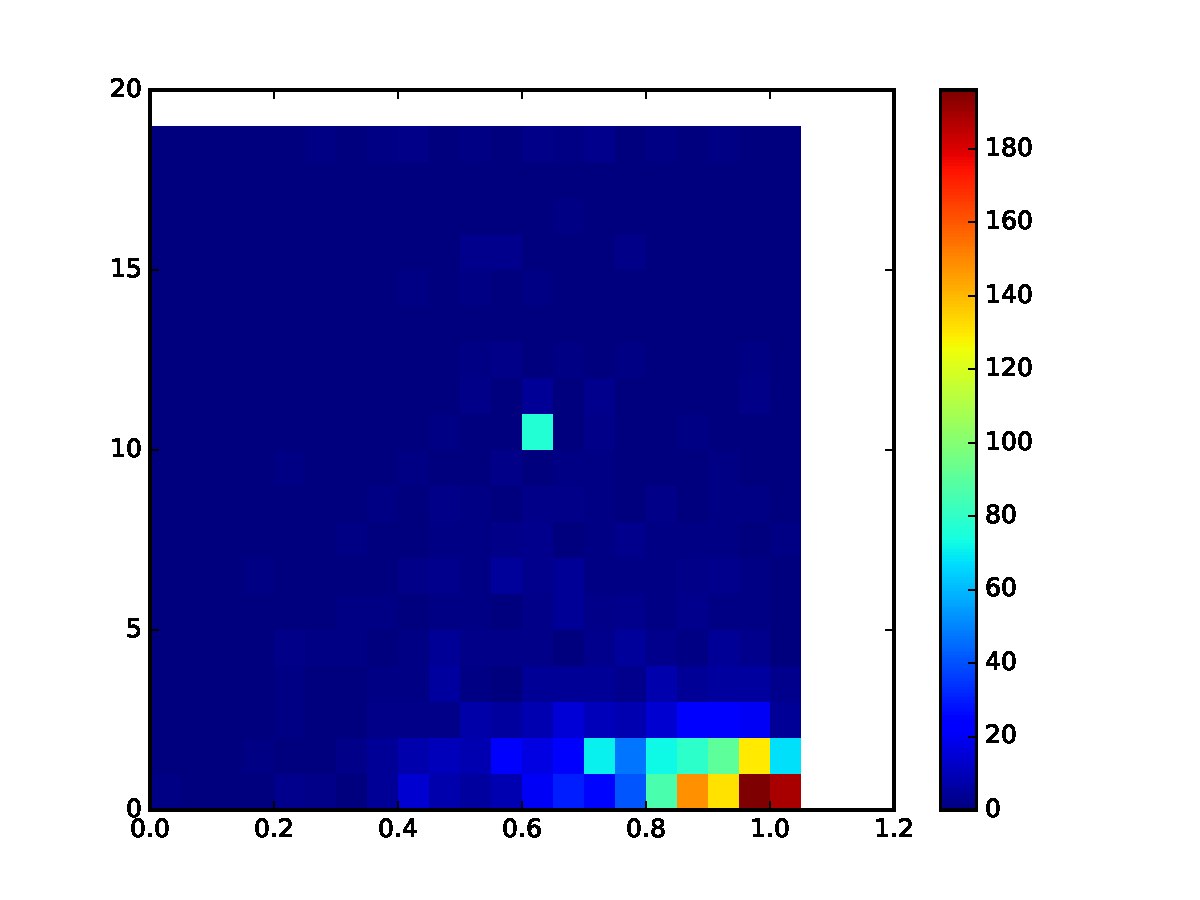
\includegraphics[keepaspectratio, scale = 0.35]{colormap_splite_3.pdf}
	 \caption{3段目のグラフ}
	 \label{third_splite_color}
	\end{minipage}
        \begin{minipage}[t]{0.45\hsize}
	 \centering
	 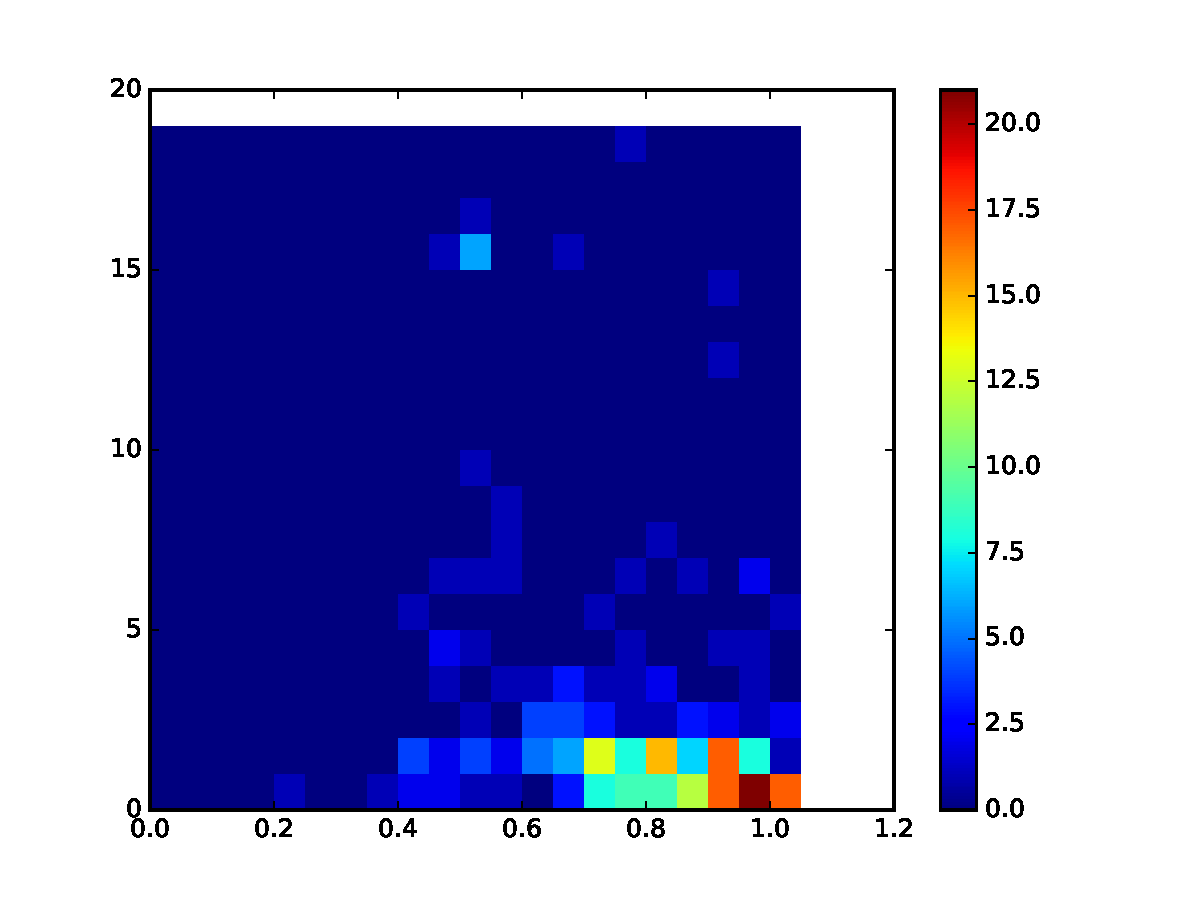
\includegraphics[keepaspectratio, scale = 0.35]{colormap_splite_4.pdf}
	 \caption{4段目のグラフ}
	 \label{fourth_splite_color}
	\end{minipage}
 \end{tabular}
 \end{figure}
 
 \section{Maze Gameプロジェクト-小規模なリミックスツリー-}
 実際に教育現場で本研究の可視化を利用する場合、クラスごとや学年ごとに授業を行うことが考えられる。教師のプログラムを生徒がリミックスし、生徒自身でオリジナルのプログラムを書き、提出するという授業形態が考えられ、リミックスツリーの規模が小さい場合も想定ができる。
 今回はMaze Gameという迷路のプログラムを使って、小規模なリミックスツリーの類似度推定も合わせて行なった。この実験では小規模であるため、1段目・2段目のみの集計となった。

 \newpage
\subsection{ブロック数とcos類似度の散布図}
 出力されたデータを元に横軸がブロック数、縦軸がcos類似度の散布図を作成した。元プロジェクト(ID:2768574)のブロック数は65で割った。2つの比較ができるように、目盛りは全ての最大値に揃えた。

\begin{figure}[h]
 \begin{tabular}{cc}
 	\begin{minipage}[t]{0.45\hsize}
	 \centering
	 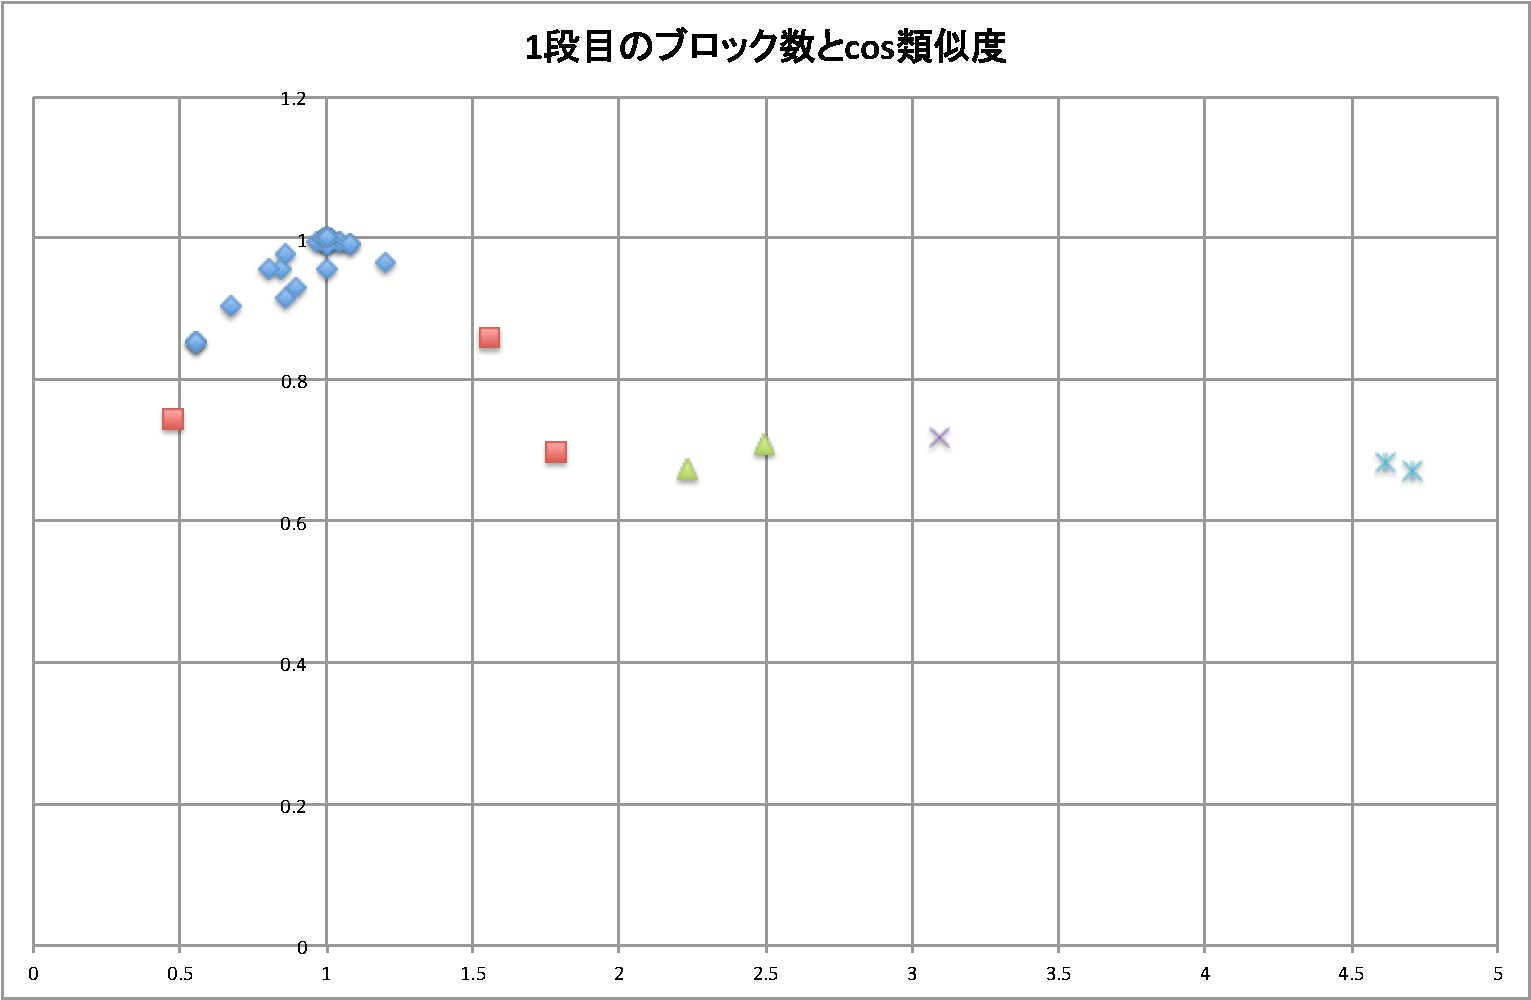
\includegraphics[keepaspectratio, scale = 0.35]{mazegame_first_block.pdf}
	 \caption{1段目のグラフ}
	 \label{mazegame_first_block_cos}
	\end{minipage}
        \begin{minipage}[t]{0.45\hsize}
	 \centering
	 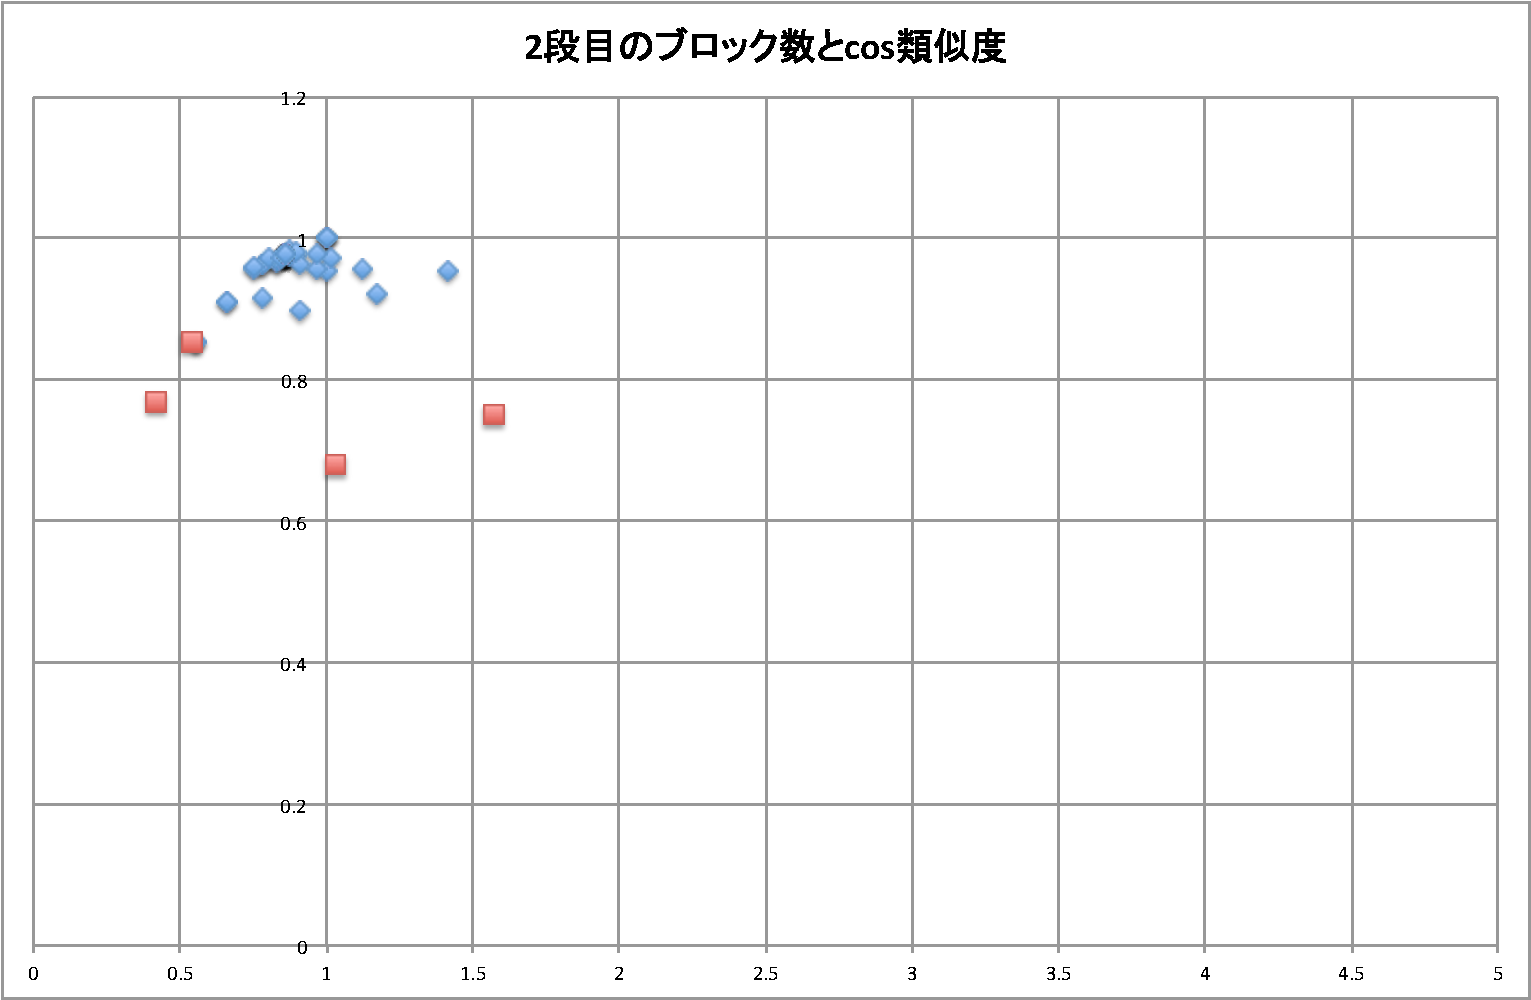
\includegraphics[keepaspectratio, scale = 0.35]{mazegame_second_block.pdf}
	 \caption{2段目のグラフ}
	 \label{mazegame_second_block_cos}
	\end{minipage}
 \end{tabular}
 \end{figure}

\subsection{スプライト数とcos類似度の散布図}
 出力されたデータを元に横軸がスプライト数、縦軸がcos類似度の散布図を作成した。元プロジェクト(ID:2768574)のスプライト数は3で割った。2つの比較ができるように、目盛りは全ての最大値に揃えた。

\begin{figure}[h]
 \begin{tabular}{cc}
 	\begin{minipage}[t]{0.45\hsize}
	 \centering
	 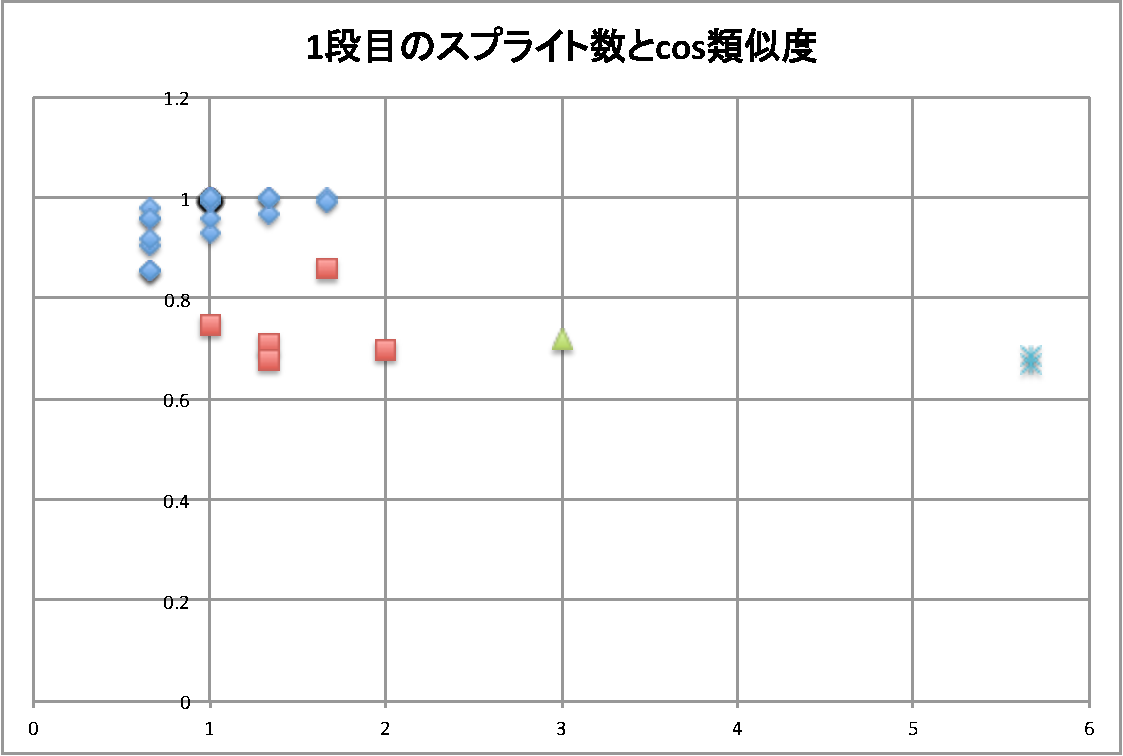
\includegraphics[keepaspectratio, scale = 0.35]{mazegame_first_splite.pdf}
	 \caption{1段目のグラフ}
	 \label{mazegame_first_splite_cos}
	\end{minipage}
        \begin{minipage}[t]{0.45\hsize}
	 \centering
	 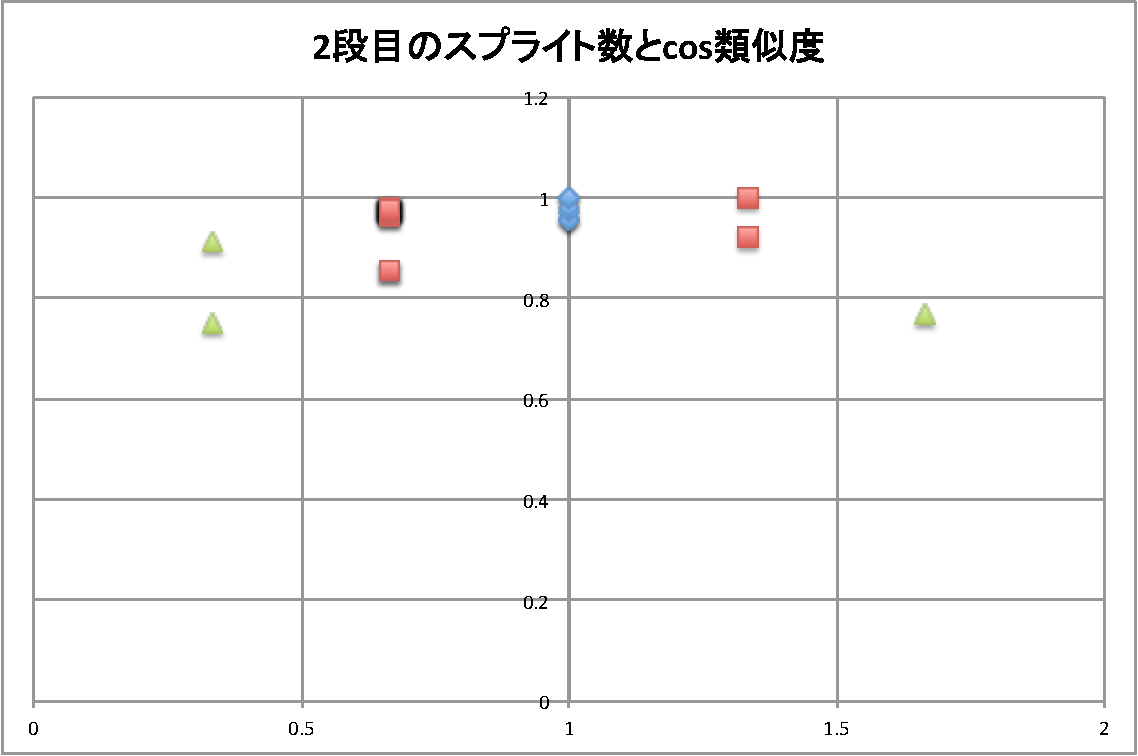
\includegraphics[keepaspectratio, scale = 0.35]{mazegame_second_splite.pdf}
	 \caption{2段目のグラフ}
	 \label{mazegame_second_splite_cos}
	\end{minipage}
 \end{tabular}
 \end{figure}

 

\chapter{評価}

\section{グラフ結果における評価}
\subsection{Pongプロジェクト-大規模なリミックスツリー-}
\subsubsection{ブロック数とスプライト数の比較}
ブロック数とスプライト数を比較すると段数が上がり、元のプログラムよりブロック数やスプライト数が多いほど類似度は低く、グラフ上では一番離れていると考えられる。つまり1段目より2段目以降が右上に点が広がっていればリミックスされ変更が加えられていることがわかる。実際の結果によるとほとんどの点が左下にある。

\subsubsection{スプライトあたりのブロック数とcos類似度の比較}
スプライトあたりのブロック数は1つのオブジェクトに対し、どれだけだけのブロックが使われているかを計算したものである。元のプロジェクトから離れるほど横軸の点は広がり、縦軸は低いところに点が存在するはずである。実際のグラフでは1段目から2段目ではこのような結果になっている。しかし1段目と3段目は点が少し広がっているがあまり変化はない。

\subsubsection{ブロック数、スプライト数とcos類似度の比較}
ブロック数、スプライト数とcos類似度の散布図では元のプロジェクト(1,1)の点から遠ざかっているほど類似していないことになる。2段目以降ではスプライトあたりのブロック数と同様に右下に広がっていればリミックスツリーと辻褄が合う。ただ実際のグラフでは1段目から2段目では広がりがわかるが、3段目ではあまり広がっていない。スプライト数とcos類似度の散布図でも同様のことがわかる。

\subsubsection{ブロック数、スプライト数とcos類似度の個数によるカラープロット}
個数の一番多い点は1段目のグラフでは(1,1)である。2段目以降、この点より内側にあるほどリミックスされたプロジェクトが元のプロジェクトだけではなく違うプロジェクトであることもわかる。図\ref{third_block_color}や\ref{fourth_block_color}にはそのような点が現れている。スプライト数とcos類似度のカラーマップでも同様に図\ref{third_splite_color}と\ref{fourth_splite_color}でも同様である。またどちらのグラフでも離れている点が3段目より4段目の方が内側にある。

\subsubsection{元のプロジェクトとの比較}
作成したグラフより、最も似ている数値のプロジェクト、最も離れている数値のプロジェクト、その中間のものを選び抜いた。最も似ているものは(1,1)にあるものが元のプロジェクトに最も近いものと判断する。1段目、2段目、4段目では(1,1)のプロジェクトが多く存在するため、その中から2つに絞る。これらのプロジェクトと元のプロジェクト(ID:10000036)を、操作・音・外装・プログラムの動き・ブロックの木構造・ゲーム終了時の6つの項目で比較し、可視化した結果が正しいかどうか検証した。(表\ref{block})(表\ref{splite})IDは色分けされており、赤が元プロジェクトと距離が近いもの、青が遠いもの、ピンクが中間のものを指す。
\\
 ブロック数とcos類似度のグラフ、スプライト数とcos類似度のグラフどちらにおいても同じような結果が出ており、それぞれの段で最も似ているもの・最も離れているもの・中間という条件で取り出したプロジェクトは、やはりよく似ている・違う・少し違う内容となっていた。よって、今回使用したブロック数・スプライト数・類似度はプロジェクト同士の類似度を図る上で重要な要素であったと言える。
\\
 また、1段目から4段目まですべてを通して見てみると、2段目以降にも元のプロジェクトと同じような内容のものが含まれていることが分かった。これは、リミックスツリーの根元(元のプロジェクト)から離れたプロジェクトも、元のプロジェクトと同じ場合が生じているということが言え、リミックスツリーではその事実までは可視化されていなかったということが伺える。本研究で行った可視化手法では、例え元のプロジェクトへいくつも遡るところに位置するプロジェクトであったとしても、ほぼ正確な類似関係が可視化できており、新たな可視化として提案できるのではないか。ここに本研究の新奇性を見出すことができた。

\newpage
\subsection{Maze Gameプロジェクト-小規模なリミックスツリー-}
\subsubsection{ブロック数、スプライト数とcos類似度の比較}
 ブロック数・スプライト数どちらのグラフも段数に限らずばらつきが見られ、一回のリミックスだけで元プロジェクトに比べて改良されているプロジェクトも複数あることが分かった。全体的に大規模なリミックスツリーと同じような傾向が見られたが、プロジェクトの量が少ないため、類似度がかなり低いプロジェクトはあまり見られなかった。
%この可視化がツール上に加わることで、それぞれの生徒がどの程度自分のアイデアでプロジェクトを作成できているか、もしくはできていないのかという新たな情報を提供でき、教育者として個々の生徒の進度を把握する一つの手助けになるのではないかと考えている。

%ブロック数とcos類似度のグラフ、スプライト数とcos類似度のグラフの表の中で、どの段においても最も似ているもの・最も離れているものはどれも共通したプロジェクトが得られたが、中間にあたるプロジェクトがどの段においても異なるという結果となった。これは、類似性を表す上で使用したブロック数とスプライト数の2つの要素によって、中間と位置付けるプロジェクトが異なったということである。本研究では2要素ごとに可視化を行ったため、このような誤差が出てしまったが、今後3次元で可視化を試みることで、改善できるのではないかと考えている。

\begin{table}[h]
 \scriptsize
 \caption{ブロック数とcos類似度のグラフの評価-大規模なリミックスツリー-}
 \label{block}
 \begin{center}
\begin{tabular}{|p{1.7cm}||p{1cm}|p{1cm}|p{1.7cm}|p{2cm}|p{1cm}|p{1.7cm}|} \hline

プロジェクトID & 操作 & 音 & 外装 & プログラムの動き & 木構造 & ゲーム終了時 \\ \hline \hline
1段目 &  &  &  &  &  &  \\ \hline
\textcolor{red}{48772890} & 同じ & 同じ & ボールの色だけ & バーが上下にも動く & 同じ & 同じ \\ \hline
\textcolor{red}{136740878} & 同じ & なくなる & 背景だけ & 同じ & 同じ & 同じ \\ \hline
\textcolor{blue}{19276295} & 同じ & 同じ & 背景・ボールの大きさ & ボールに触れたら負け、コウモリを跳ね返してボールが下に落ちないようにする & 違う & 負けても終わらない \\ \hline
\textcolor{magenta}{14377547} & 同じ & 同じ & 背景・ボールの色 & バーにボールが当たるとポイントが加算される & 違う & 同じ \\ \hline

2段目 &  &  &  &  &  &  \\ \hline
\textcolor{red}{10630533} & 同じ & 違う & 背景・ボール・バー & 同じ & ほぼ同じ & 同じ \\ \hline
\textcolor{red}{20087979} & 同じ & 違う & 背景・ボール・バー & 同じ & ほぼ同じ & 音が鳴り、もう一度動き始める \\ \hline
\textcolor{blue}{73001742} & なくなる & 違う & ボールが複数・バーも2種類 & ボールが同時にたくさん動き、ユーザがバーを動かせないようになっている & ほぼ同じ & なし \\ \hline
\textcolor{magenta}{31314852} & 同じ & 同じ & 背景・ボール・バー & バーに当たるとポイントがたまるが、バーに当たらないと地面に当たって跳ね返る & 違う & 何回か落ちてゲームオーバー画面になる \\ \hline

3段目 &  &  &  &  &  &  \\ \hline
\textcolor{red}{97570310} & 同じ & なし & 背景・ボール & 同じ & 同じ & 同じ \\ \hline
\textcolor{blue}{71289464} & なくなる & なし & 背景・ボール・ポイント3種 & ボールが勝手に動着続ける & 違う & 終了しない \\ \hline
\textcolor{magenta}{70556576} & なくなる & なし & 背景・ボールが複数・ポイント & 全く動かない & 少し違う & 終了しない \\ \hline

4段目 &  &  &  &  &  &  \\ \hline
\textcolor{red}{11534736} & 同じ & 同じ & 背景・ボール & 同じ & 同じ & 同じ \\ \hline
\textcolor{red}{23516253} & 同じ & 違う & 背景・ボール & 同じ & 同じ & 跳ね返り続けられる \\ \hline
\textcolor{blue}{44740270} & なくなる & なし & 背景・ボール・ポイント & なくなる & 少し違う & なくなる \\ \hline
\textcolor{magenta}{118943024} & 2人用になりキーボードで操作する & なし & 背景・ボール・バー・ポイント & バー2つ、ボール2つでボールが落ちないように操作をし、 途中からボールが早くなる、片方にはポイントはたまるが、もう片方には入らない & 違う & ポイントがたまっても終わらない \\ \hline

\end{tabular}
\end{center}
\end{table}

\begin{table}[h]
 \scriptsize
 \caption{スプライト数とcos類似度のグラフの評価-大規模なリミックスツリー-}
 \label{splite}
 \begin{center}
\begin{tabular}{|p{1.7cm}||p{1cm}|p{1cm}|p{1.7cm}|p{2cm}|p{1cm}|p{1.7cm}|} \hline

プロジェクトID & 操作 & 音 & 外装 & プログラムの動き & 木構造 & ゲーム終了時 \\ \hline \hline
1段目 &  &  &  &  &  &  \\ \hline
\textcolor{red}{48772890} & 同じ & 同じ & ボールの色だけ & バーが上下にも動く & 同じ & 同じ \\ \hline
\textcolor{red}{136740878} & 同じ & なくなる & 背景だけ & 同じ & 同じ & 同じ \\ \hline
\textcolor{blue}{19276295} & 同じ & 同じ & 背景・ボールの大きさ & ボールに触れたら負け、コウモリを跳ね返してボールが下に落ちないようにする & 違う & 負けても終わらない \\ \hline
\textcolor{magenta}{90709078} & 同じ & 同じ & ボール・バーが複数・ポイント3種 & 複数のボールが一斉に動く & 違う & 同じ \\ \hline

2段目 &  &  &  &  &  &  \\ \hline
\textcolor{red}{10630533} & 同じ & 違う & 背景・ボール・バー & 同じ & ほぼ同じ & 同じ \\ \hline
\textcolor{red}{20087979} & 同じ & 違う & 背景・ボール・バー & 同じ & ほぼ同じ & 音が鳴り、もう一度動き始める \\ \hline
\textcolor{blue}{73001742} & なくなる & 違う & ボールが複数・バーも2種類 & ボールが同時にたくさん動き、ユーザがバーを動かせないようになっている & ほぼ同じ & なし \\ \hline
\textcolor{magenta}{70556576} & なくなる & なくなる & 背景、ボール & 全く動かない & 少し違う & ゲームが始まらない \\ \hline

3段目 &  &  &  &  &  &  \\ \hline
\textcolor{red}{97570310} & 同じ & なし & 背景・ボール & 同じ & 同じ & 同じ \\ \hline
\textcolor{blue}{71289464} & なくなる & なし & 背景・ボール・ポイント3種 & ボールが勝手に動着続ける & 違う & 終了しない \\ \hline
\textcolor{magenta}{33903574} & 同じ & 新たな音が追加 & 背景・ボールの色・バーの色 & スコア付き & 違う & ゲーム終了時に音が鳴る \\ \hline

4段目 &  &  &  &  &  &  \\ \hline
\textcolor{red}{11534736} & 同じ & 同じ & 背景・ボール & 同じ & 同じ & 同じ \\ \hline
\textcolor{red}{23516253} & 同じ & 違う & 背景・ボール & 同じ & 同じ & 跳ね返り続けられる \\ \hline
\textcolor{blue}{44740270} & なくなる & なし & 背景・ボール・ポイント & なくなる & 少し違う & なくなる \\ \hline
\textcolor{magenta}{134337312} & なくなる & なし & 背景 & なくなる & 違う & ゲームが始まらない \\ \hline

\end{tabular}
\end{center}
\end{table}

\newpage
\section{第三者による評価}
\subsection{評価方法}
 大規模なリミックスツリーにおいて評価するために抽出したプロジェクトが、第三者は元プロジェクトと比べてどのように評価するか、Scratchの専門家2名と情報科学を学ぶ学生5人にアンケートをとった。
 方法としては、アンケートフォーラムを用意し収集した。アンケート内容は、  \label{block}もしくは\label{splite}で抽出したプロジェクトの内1段目から4段目の最も似ている数値のプロジェクト、最も離れている数値のプロジェクト、その中間、合計16個のプロジェクトと元プロジェクトを実際に動かし、似ているか似ていないかを5段階評価してもらう。アンケート回答者にはそれぞれのプロジェクトは何段目のものなのかは伏せ、並列した数字(ゲーム1〜ゲーム16)で表示した。
%
%%% 謝辞
\chapter{謝辞}
\addcontentsline{toc}{chapter}{謝辞}
本研究を進めるにあたり、日々丁寧かつ熱心なご指導を来住伸子教授から賜りました。また青山学院大学の吉田葵助教授にも貴重な時間を割いていただきアドバイスをいただきましたここに感謝の意を表します。


%
%

\begin{thebibliography}{21}

%\bibitem{a} \lceil title \rfloor, \langle url \rangle, xxxx/xx/xxアクセス
\bibitem{it_edu}教育・学習分野の情報化に係る国内外の動向と先進事例, 総務省 http://www.kknews.co.jp/maruti/news/2014/0804\_4a.html
\bibitem{edu_prog}小学校でプログラミング アイデアを形にする力をつける (2014年8月4日), 教育課程新聞 http://www.kknews.co.jp/maruti/news/2014/0804\_4a.html
\bibitem{preEssay1}森秀樹・杉澤学・張海・前迫孝憲(2011)「Scratchを用いた小学校プログラミング授業の実践〜小学生を対象としたプログラミング教育の再考〜」
\bibitem{preEssay2}小田悠介、若林茂(2013年) 「プログラム間の類似性の定量化手法」,[online]http://www.kobe-kosen.ac.jp/activity/publication/kiyou/Kiyou12/Data/Vol51Paper103-108.pdf
\bibitem{scratch}Scratch - Imagine, Program, Share, MIT Media Lab https://scratch.mit.edu/
\bibitem{scratch_official}Scratch Offline Editor, MIT Media Lab https://scratch.mit.edu/scratch2download/
\bibitem{scratch_article}Scratchで始めるプログラミング教育(1):プログラミングを学習する意義、Scratchの基本的な使い方超入門 (2016年3月21日), 薬師寺国安 http://www.atmarkit.co.jp/ait/articles/1603/21/news012.html
\bibitem{scratch_about}Scratch - Imagine, Program, Share, Scratchについて, MIT Media Lab https://scratch.mit.edu/about
\bibitem{pongret}Remix tree for Pong Starter https://scratch.mit.edu/projects/10000036/remixtree/
\bibitem{python}はじめに|学生のためのPython講座 http://python4study.9isnine.com/first
\bibitem{json}JSONってなにもの?(2008), 竹添直樹 https://thinkit.co.jp/article/70/1
\bibitem{json_py}【Python入門】JSON形式データの扱い方 (2016年12月12日), Morio http://qiita.com/Morio/items/7538a939cc441367070d
\bibitem{cos} コサイン類似度 http://www.cse.kyoto-su.ac.jp/~g0846020/keywords/cosinSimilarity.html
\bibitem{tf_idf_cos} TF-IDF Cos類似度推定法 - Qiita (2015年8月24日), nmbakfm http://qiita.com/nmbakfm/items/6bb91b89571dd68fcea6
\bibitem{simcalc} Python3.3で実装したナイーブベイズ分類器を利用して文章と文字列中の語の共起頻度から、類似度を計算する (2013年12月26日), katryo http://qiita.com/katryo/items/b6962facf744e93735bb
\bibitem{urllib} 20.6. urllib2 ー URLを開くための拡張可能なライブラリ (原文) (2017年1月2日), Python Software Foundation http://docs.python.jp/2/library/urllib2.html
\bibitem{isinstance} 2. 組み込み関数 ー Python2.7.x ドキュメント (2017年1月2日), Python Software Foundation http://docs.python.jp/2/library/functions.html\#isinstance
\bibitem{open} 2. 組み込み関数 ー Python2.7.x ドキュメント (2017年1月2日), http://docs.python.jp/2/library/functions.html\#open
\bibitem{unicode} Unicode文字列(ユニコード文字列) - 文字列 - PythonWeb, TATSUO IKURA, http://www.pythonweb.jp/tutorial/string/index5.html
\bibitem{rstrip} 5. 組み込み型 ー Python2.7.x ドキュメント (2017年1月2日), http://docs.python.jp/2/library/stdtypes.html?highlight=rstrip\#str.rstrip
\bibitem{loads} 18.2. json ー JSON エンコーダおよびデコーダ (原文) ー Python2.7.x ドキュメント (2017年1月2日), http://docs.python.jp/2/library/json.html




\end{thebibliography}

\newpage
\appendix
\chapter{}
\lstinputlisting[caption=SimCalculator.py,label=scprog]{SimCalculator.py}
\lstinputlisting[caption=scratchAnalysis.py,label=saprog]{scratchAnalysis.py}
\lstinputlisting[caption=scratch\_block.py,label=sbprog]{scratch_block.py}
\newpage
%\lstinputlisting[caption=data\_to\_cross.py,label=dcroprog]{data_to_cross.py}
%\lstinputlisting[caption=data\_to\_graph.py,label=dgprog]{data_to_graph.py}

\newpage
\printindex
%
%
\end{document}

